\chapter{Алгоритми при прогнозиране и обучение на изкуствени невронни мрежи}

\section{Ограничения в пространството на променливите}

Теглата в класическия многослоен перцептрон са реални числа, като не се поставят ограничения за техните стойности. Теглата могат да варират от големи отрицателни числа до големи положителни числа. Стойностите на тези тегла най-често се представят в матрица, стълбовете и редовете на която матрица показват кой неврон с кой неврон е свързан, чрез конкретно тегло в ред и стълб. При популационните оптимизационни алгоритми се работи с вектори (индивидите в популацията), така че матрицата бива представена като вектор. Задачата за търсене на оптимални стойности на теглата не поставя ограничения за самите стойности, но когато оптимизацията се извършва при поставени ограничения, и най-вече нелинейни ограничения, то популационните оптимизационни алгоритми лесно изпадат в локални оптимуми или в невъзможност да генерират допустими решения. За да се избегнат тези две трудности може да се въведе подход за допълнителна популация (пул от кандидат решения), където да се съхраняват всички допустими решения в процеса на еволюиране. Класическият подход за отразяване на факта, че едно решение (индивид) в основната популация е недопустимо, става чрез въвеждане на санкция (penalty). Санкцията е някаква форма на числено влошаване на жизнената стойност, присвоена на индивида. Наличието на санкции в популацията възпрепятства присъствието на недопустими решения и по този начин тласка алгоритъма към изпадане в локални оптимуми. Получава се така, че допустимите решения доминират недопустимите решения, а за ефективно изследване на пространството е от съществено значение алгоритъмът да може да преминава през недопустими решения, така че да достигне до следващи (неизвестни до сега) допустими решения. Този пул от допустими решения може да се използва на определени интервали от време за внасяне на генетично разнообразие в основната популация. За да се избегне израждането на основната популация, а и на пула с допустими решения, то на всеки индивид освен жизнена стойност може да се постави характеристика за стареене (aging). Коефициентът за стареене е своеобразна вероятност за изборът на индивида в процеса по селекция, при създаването на следващи поколения. Колкото по-дълго е стоял индивидът в основната популация и в пула с допустими решения, толкова по-малка е вероятността този индивид да бъде избран за бъдещо репродуциране. Пулът с допустими решения има и вторична роля, която е свързана с предлагане на решение след приключване на оптимизационния процес. Имайки ролята на операция за елит, най-доброто решение в този пул се предлага като окончателен резултат от оптимизацията. 

\section{Оператор за селекция с локално търсене, пълно изчерпване и рекурсивно спускане}

Генетичните алгоритми са глобална оптимизационна мета-евристика, вдъхновена от идеите в естествената еволюция. Процесът на оптимизация е организиран в три общи операции - селекция, кръстосване и мутация. Кръстосването и мутацията са отговорни за предлагането на нови решения в популацията, а селекцията е отговорна за по -добър избор на родители. През последните пет десетилетия в литературата са предложени много оператори за селекция - пропорционална селекция, турнирна слекция, ранг базиран селекция, болцманова селекция, слекция с нелинейно класиране, конкурентна селекция и други. Тук се предлага нов оператор за селекция, основан на създаването на рекурсивни поколения. На всяко ниво на рекурсия всички индивиди в популацията се чифтосват помежду си (груба сила). Методът на грубата сила се комбинира с локално търсене, като груба сила се прилага докато има излъчване на по-добър индивид в поколението\begin{comment}\cite{Balabanov-01}\end{comment}. Само най-добрият индивид се изкачва в по-горното ниво на рекурсията. 

\begin{lstlisting}[caption=Равномерно кръстосване, language=Java, basicstyle=\tiny, label=list0011]
	static double[] crossover(double first[], double second[]) {
		double[] child = new double[INPUT_SIZE];

		for (int i = 0; i < INPUT_SIZE; i++) {
			if (PRNG.nextBoolean()) {
				child[i] = first[i];
			} else {
				child[i] = second[i];
			}
		}

		return child;
	}
\end{lstlisting}

\begin{lstlisting}[caption=Мутация със случайно число, language=Java, basicstyle=\tiny, label=list0012]
	static void mutate(double child[]) {
		for (int i = 0; i < INPUT_SIZE; i++) {
			if (PRNG.nextDouble() >= MUTATION_RATE) {
				continue;
			}

			child[i] += PRNG.nextDouble() - 0.5D;
		}
	}
\end{lstlisting}

Популацията в генетичния алгоритъм е организирана като йерархична структура. На най-ниското ниво на структурата популацията се състои от произволно генерирани индивиди (Листинг \ref{list0013}). Във всяка популация всеки индивид се чифтосват с всички други (кръстосване - Листинг \ref{list0011} и мутация - Листинг \ref{list0012}). Само най-жизненият индивид се изпраща към по-горното ниво на рекурсивната структура (Листинг \ref{list0013}). По този начин всяка по-горна популация се установява от най-добрите индивиди, изпратени от по-долните нива.

\begin{lstlisting}[caption=Йерархична селекция, language=Java, basicstyle=\tiny, label=list0013]
	private static double[] solution(int depth, int size, Selection selection,
			Function function) {
		double[] result = null;

		if (depth > 0) {
			double population[][] = new double[size][];
			for (int j = 0; j < size; j++) {
				population[j] = solution(depth - 1, size, selection, function);
			}

			result = selection.best(population, function);
		} else if (depth == 0) {
			/* First generation is selected randomly. */
			result = new double[INPUT_SIZE];
			for (int i = 0; i < INPUT_SIZE; i++) {
				result[i] = function.minimum() + PRNG.nextDouble()
						* (function.maximum() - function.minimum());
			}
		}

		return result;
	}
\end{lstlisting}

Като тестове се взети функциите общо известни функции за проверка на евристични оптимизационни алгоритми (Michalewicz, Ackley, Schwefel Rastrigin, Griewank \cite{Balabanov-01}). Всички експерименти се извършват в 10K пространствено реално число \cite{Tomov-01}. Подобрението постигнато с добавянето на локално търсене, спрямо варианта използващ единствено пълно изчерпване е илюстрирано в Таблица \ref{tab0001}.

\begin{table}[h!]
\begin{tabular}{ | c | c | c | c | c | c | }
\hline
& \cellcolor{gray!15}Michalewicz & \cellcolor{gray!15}Ackley & \cellcolor{gray!15}Schwefel & \cellcolor{gray!15}Rastrigin & \cellcolor{gray!15}Griewank \\ [0.05ex] 
\hline
\hline
Local Search & 1062492546 & 531027435 & 533232986 & 507650704 & 592370933 \\  
\hline
Brute-Force & 403141211 & 166733879 & 175069174 & 159862955 & 218428047 \\  
\hline
\end{tabular}
\caption{Време за изчисление [ms] при ниво на рекурсия 7 и размер на популацията 11}
\label{tab0001}
\end{table}

Експериментите са проведени при ниво на рекурсия 7 и размер на популацията 11. В Таблица \ref{tab0002} са визуализирани броя изчисления на целевата функция, спрямо вида алгоритъм, за всяка от тестовите функции. 

\begin{table}[h!]
\begin{tabular}{ | c | c | c | c | c | c | }
\hline
& \cellcolor{gray!15}Michalewicz & \cellcolor{gray!15}Ackley & \cellcolor{gray!15}Schwefel & \cellcolor{gray!15}Rastrigin & \cellcolor{gray!15}Griewank \\ [0.05ex] 
\hline
\hline
Local Search & 641125639 & 641024362 & 640914978 & 641092606 & 640830762 \\  
\hline
Brute-Force & 235794757 & 235794757 & 235794757 & 235794757 & 235794757 \\  
\hline
\end{tabular}
\caption{Брой изчисления на целевата функция при ниво на рекурсия 7 и размер на популацията 11}
\label{tab0002}
\end{table}

Броят изчисления на целевата функция не може да бъде предварително определен във варианта, когато се прилага локално търсене \cite{Tomov-02}. Достигнатите субоптимални стойности за всяка от функциите, при ниво на рекурсия 7 и размер на популацията 11, са представени в Таблица \ref{tab0003}. Таблично са представени граничния случай с ниво на рекурсия 7 и размер на популацията 11. Графично се представят резултатите от експериментите проведени за нива на рекурсия от 2 до 7 и размери на популацията от 2 до 11 (Фиг. \ref{fig0019}-\ref{fig0048}).

\begin{table}[h!]
\begin{tabular}{ | c | c | c | c | }
\hline
& \cellcolor{gray!15}Michalewicz & \cellcolor{gray!15}Ackley & \cellcolor{gray!15}Schwefel \\ [0.05ex] 
\hline
\hline
Local Search & -1484.7137949531716 & 21.09334816052046 & 3877924.0971615044 \\  
\hline
Brute-Force & -1439.2296970724608 & 21.114702255301292 & 3919318.729777085 \\  
\hline
\hline
& \cellcolor{gray!15}Rastrigin & \cellcolor{gray!15}Griewank & \\ [0.05ex] 
\hline
\hline
Local Search & 170204.87849875208 & 259918.15469527297 & \\  
\hline
Brute-Force & 171780.33307271387 & 262621.61053178157 & \\  
\hline
\end{tabular}
\caption{Изчислени субоптимални стойности при ниво на рекурсия 7 и размер на популацията 11}
\label{tab0003}
\end{table}

%\begin{figure}[H]
%  \centering
%  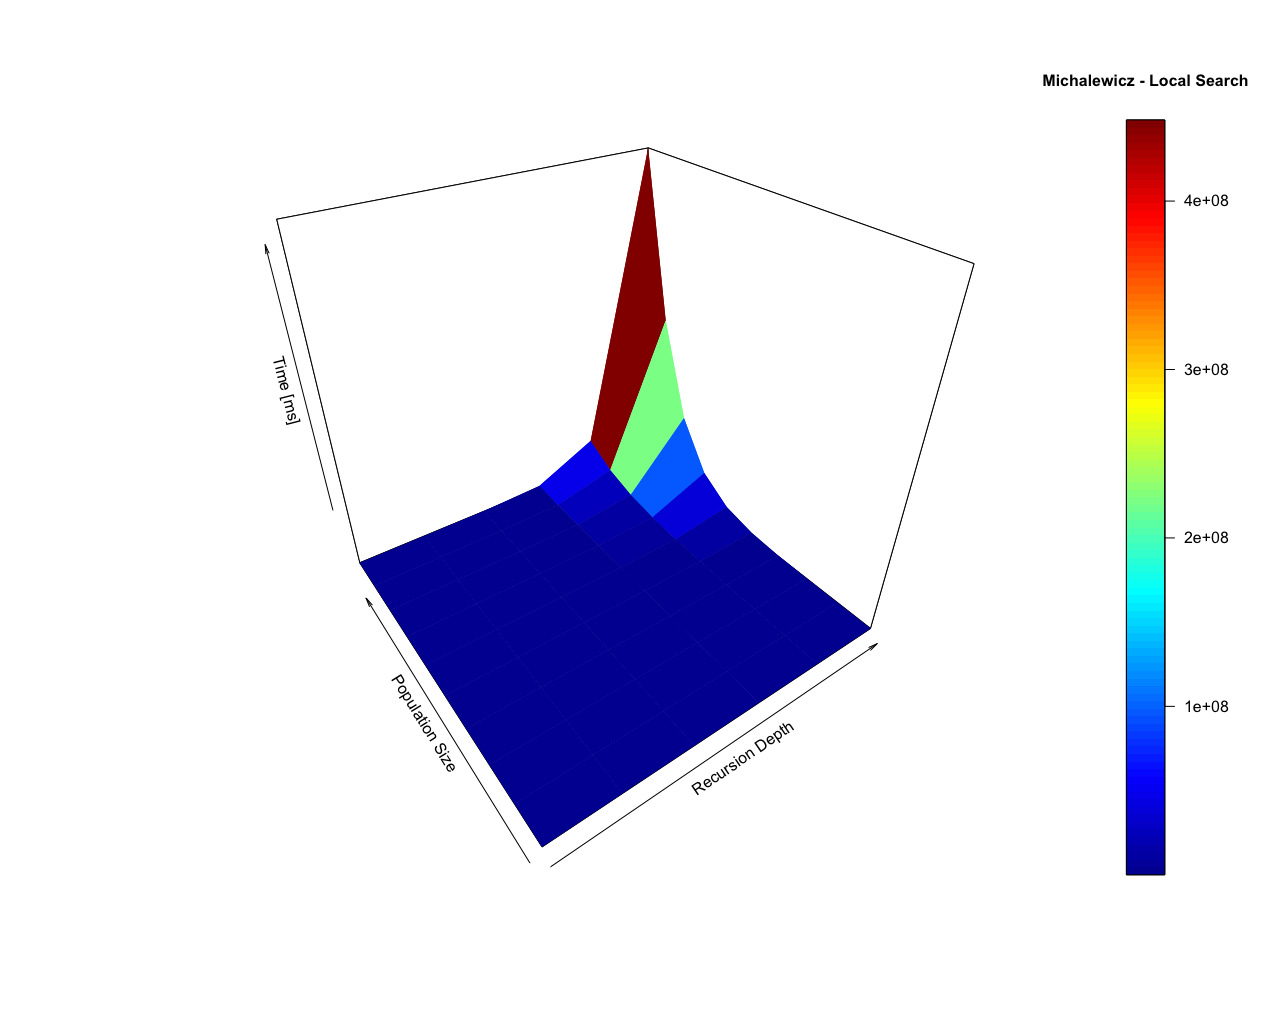
\includegraphics[width=0.8\linewidth]{fig0019.png}
%  \caption{Изчислително време [ms] за функцията Michalewicz с локално търсене}
%\label{fig0019}
%\end{figure}
%
%\begin{figure}[H]
%  \centering
%  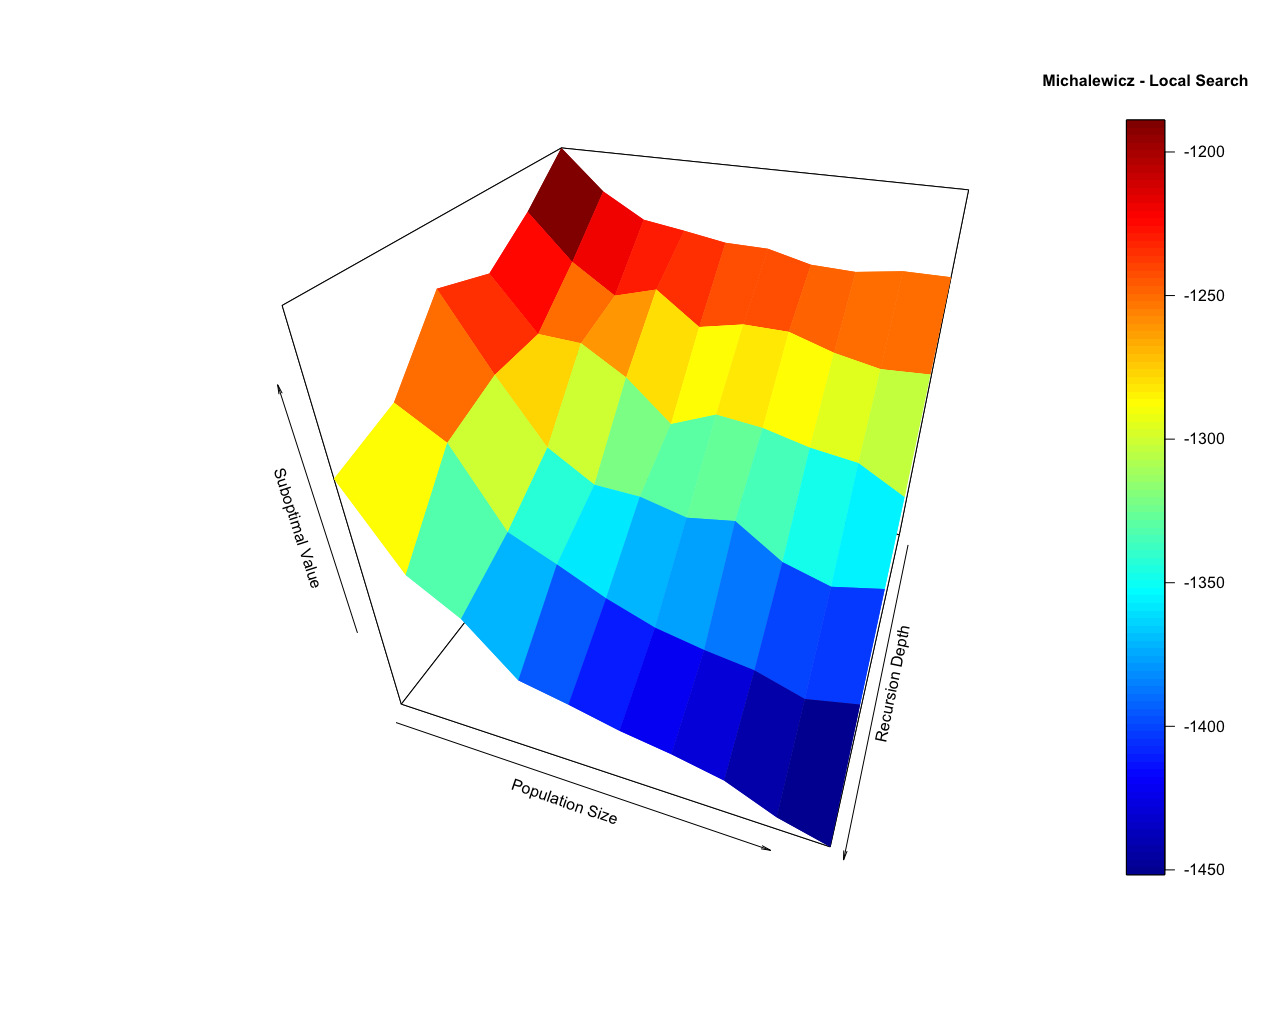
\includegraphics[width=0.8\linewidth]{fig0020.png}
%  \caption{Субоптимални стойности за функцията Michalewicz с локално търсене}
%\label{fig0020}
%\end{figure}
%
%\begin{figure}[H]
%  \centering
%  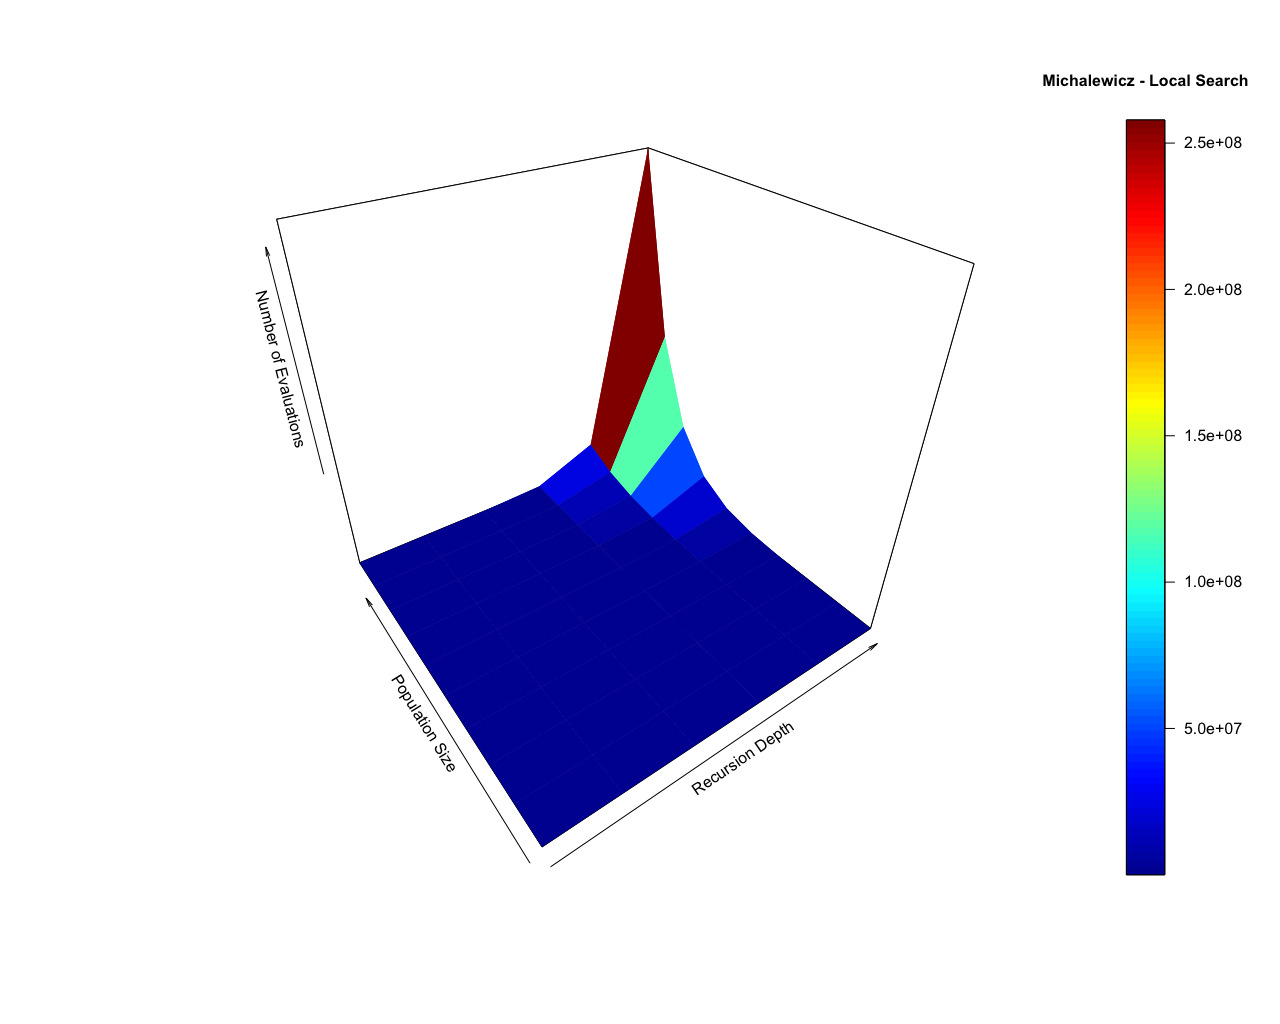
\includegraphics[width=0.8\linewidth]{fig0021.png}
%  \caption{Брой изчисления на функцията Michalewicz с локално търсене}
%\label{fig0021}
%\end{figure}
%
%\begin{figure}[H]
%  \centering
%  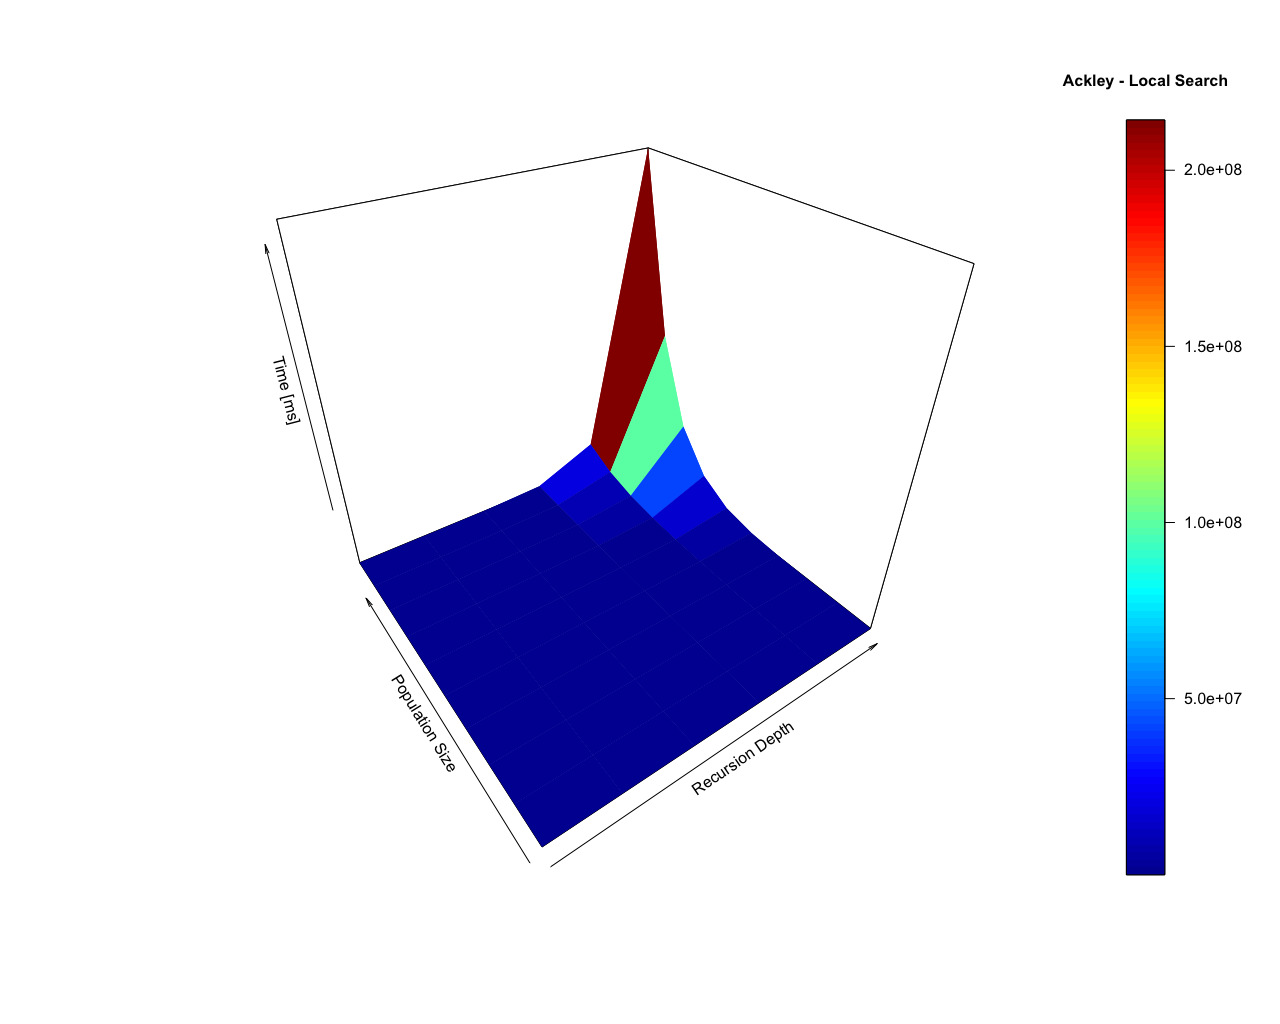
\includegraphics[width=0.8\linewidth]{fig0022.png}
%  \caption{Изчислително време [ms] за функцията Ackley с локално търсене}
%\label{fig0022}
%\end{figure}
%
%\begin{figure}[H]
%  \centering
%  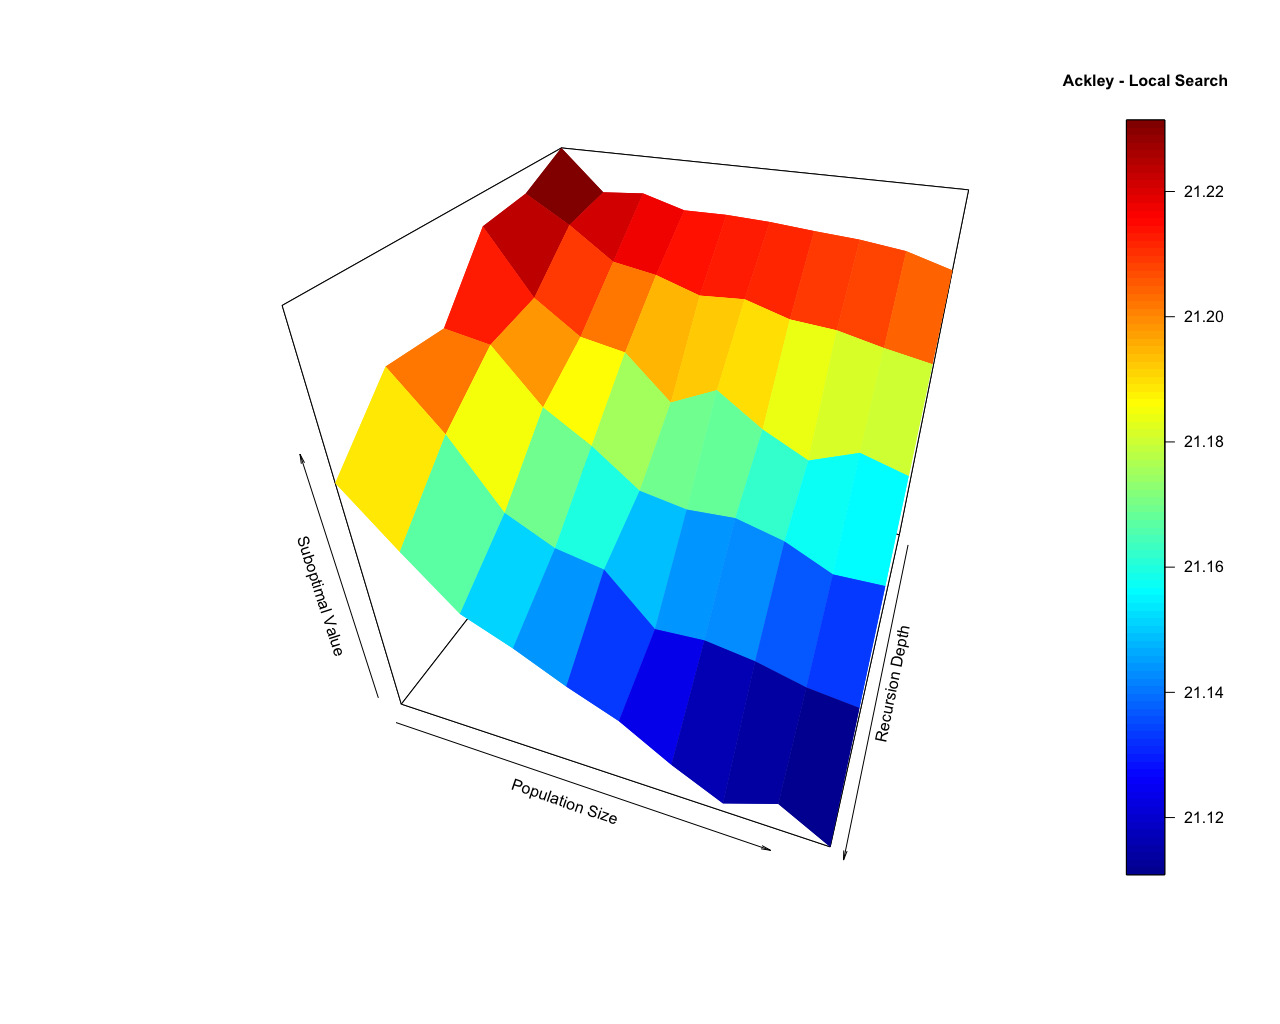
\includegraphics[width=0.8\linewidth]{fig0023.png}
%  \caption{Субоптимални стойности за функцията Ackley с локално търсене}
%\label{fig0023}
%\end{figure}
%
%\begin{figure}[H]
%  \centering
%  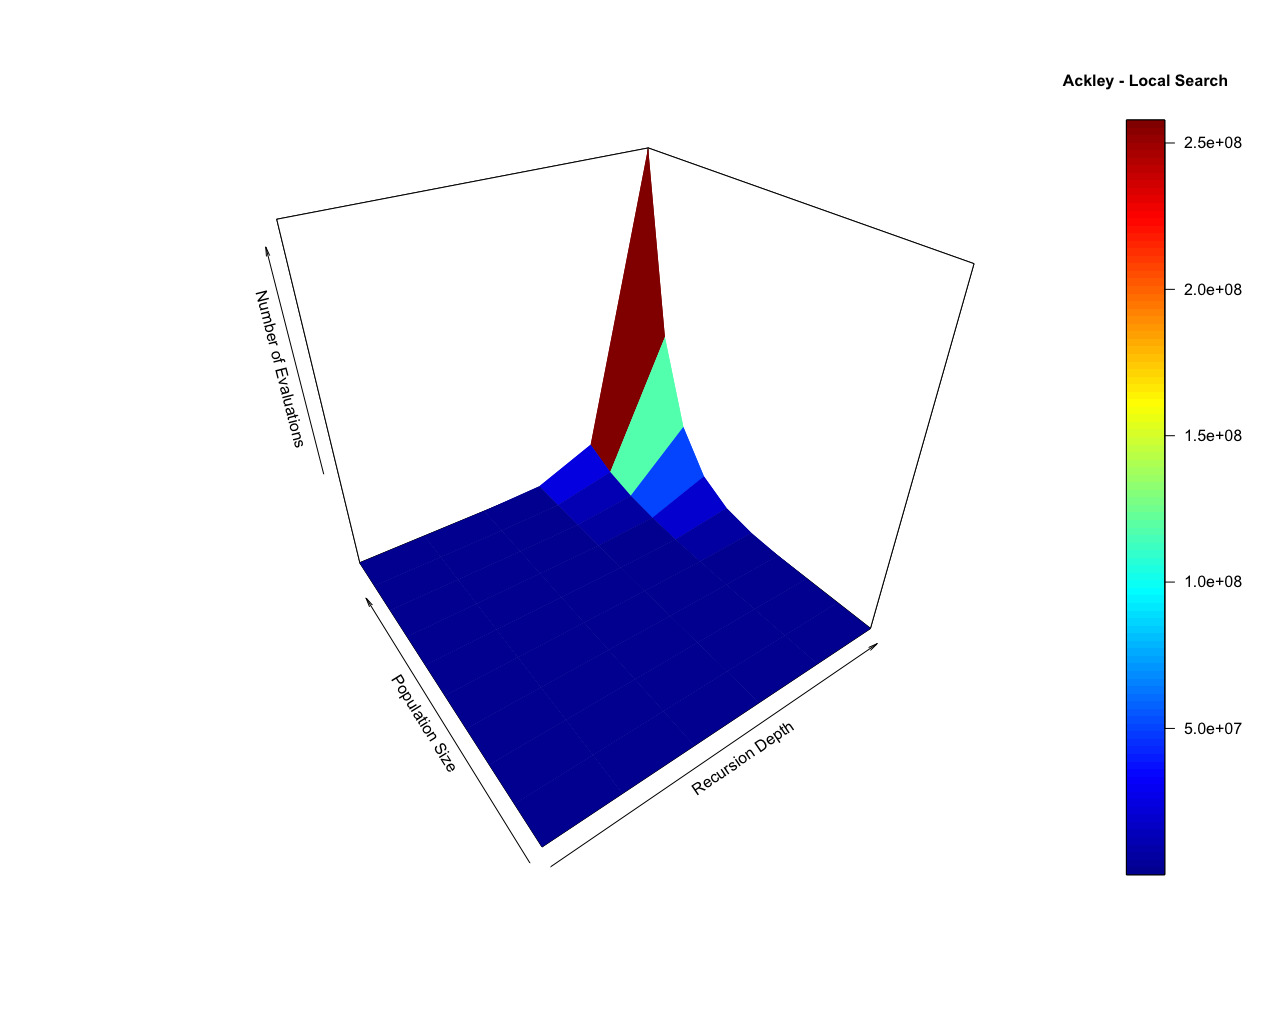
\includegraphics[width=0.8\linewidth]{fig0024.png}
%  \caption{Брой изчисления на функцията Ackley с локално търсене}
%\label{fig0024}
%\end{figure}
%
%\begin{figure}[H]
%  \centering
%  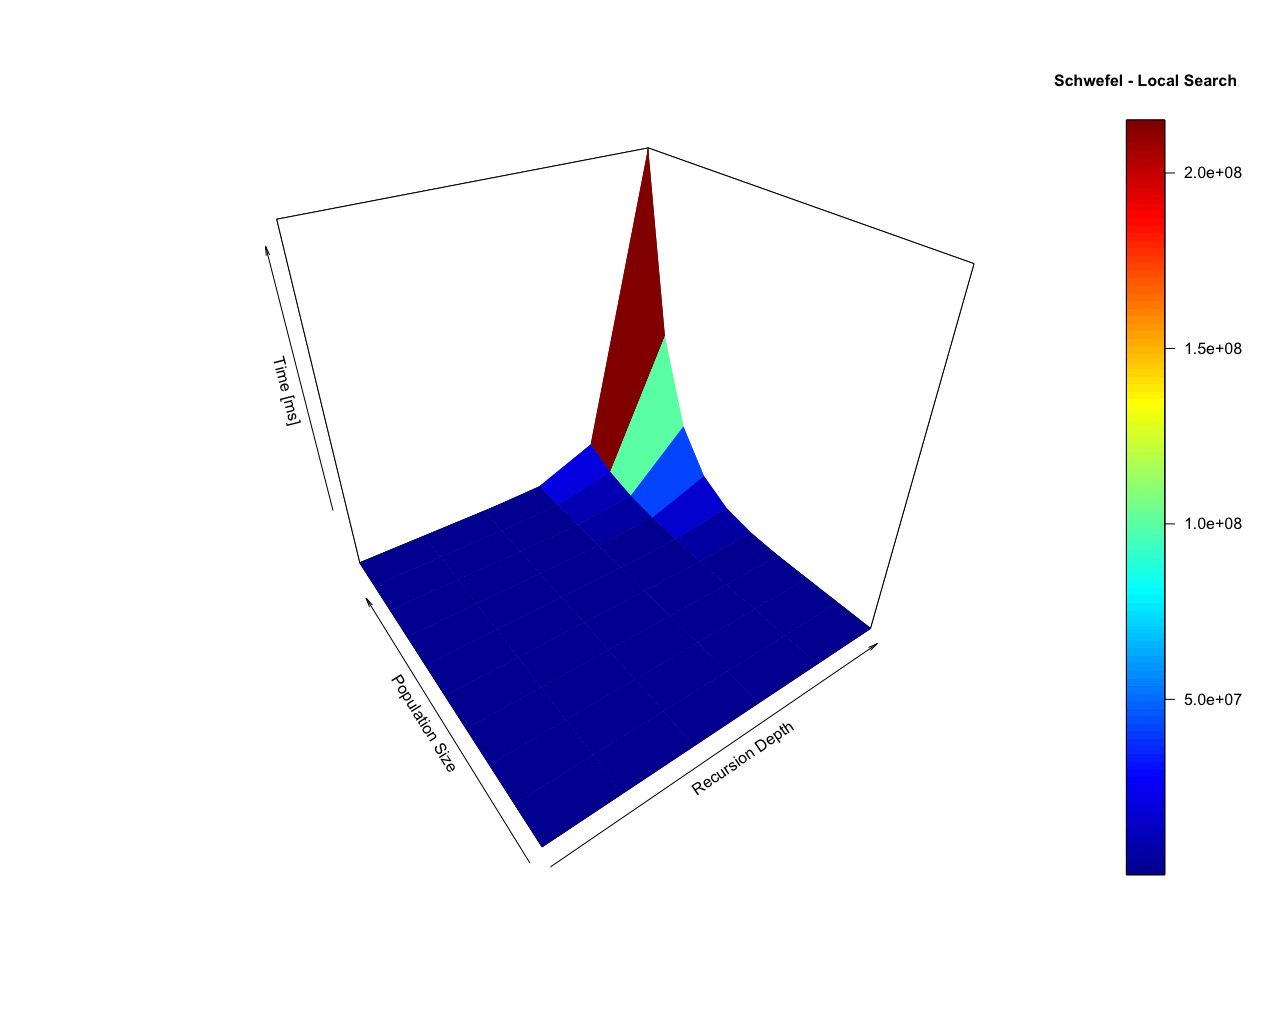
\includegraphics[width=0.8\linewidth]{fig0025.png}
%  \caption{Изчислително време [ms] за функцията Schwefel с локално търсене}
%\label{fig0025}
%\end{figure}
%
%\begin{figure}[H]
%  \centering
%  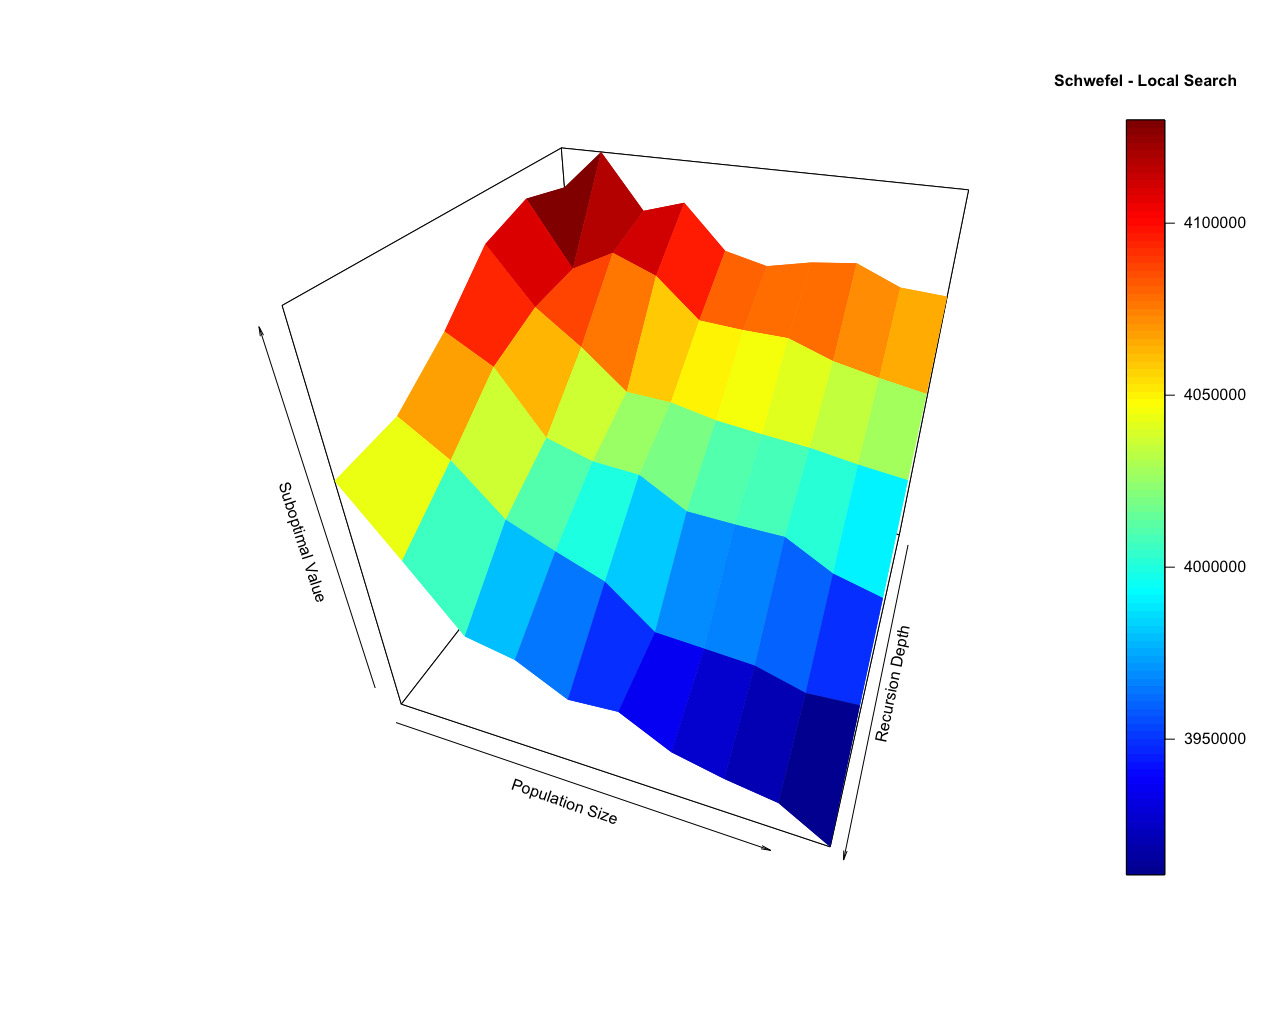
\includegraphics[width=0.8\linewidth]{fig0026.png}
%  \caption{Субоптимални стойности за функцията Schwefel с локално търсене}
%\label{fig0026}
%\end{figure}
%
%\begin{figure}[H]
%  \centering
%  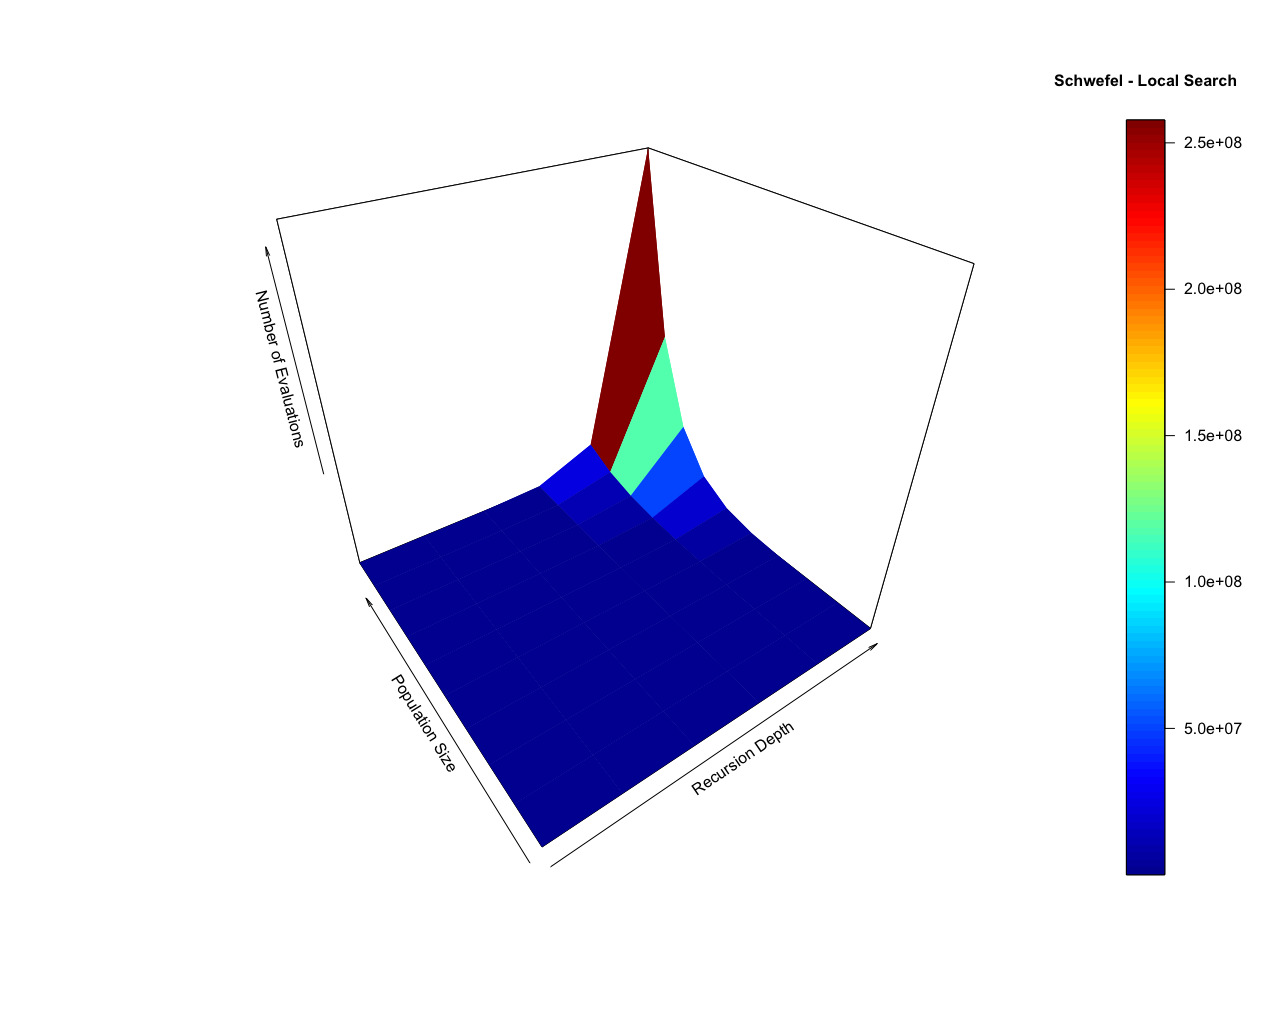
\includegraphics[width=0.8\linewidth]{fig0027.png}
%  \caption{Брой изчисления на функцията Schwefel с локално търсене}
%\label{fig0027}
%\end{figure}
%
%\begin{figure}[H]
%  \centering
%  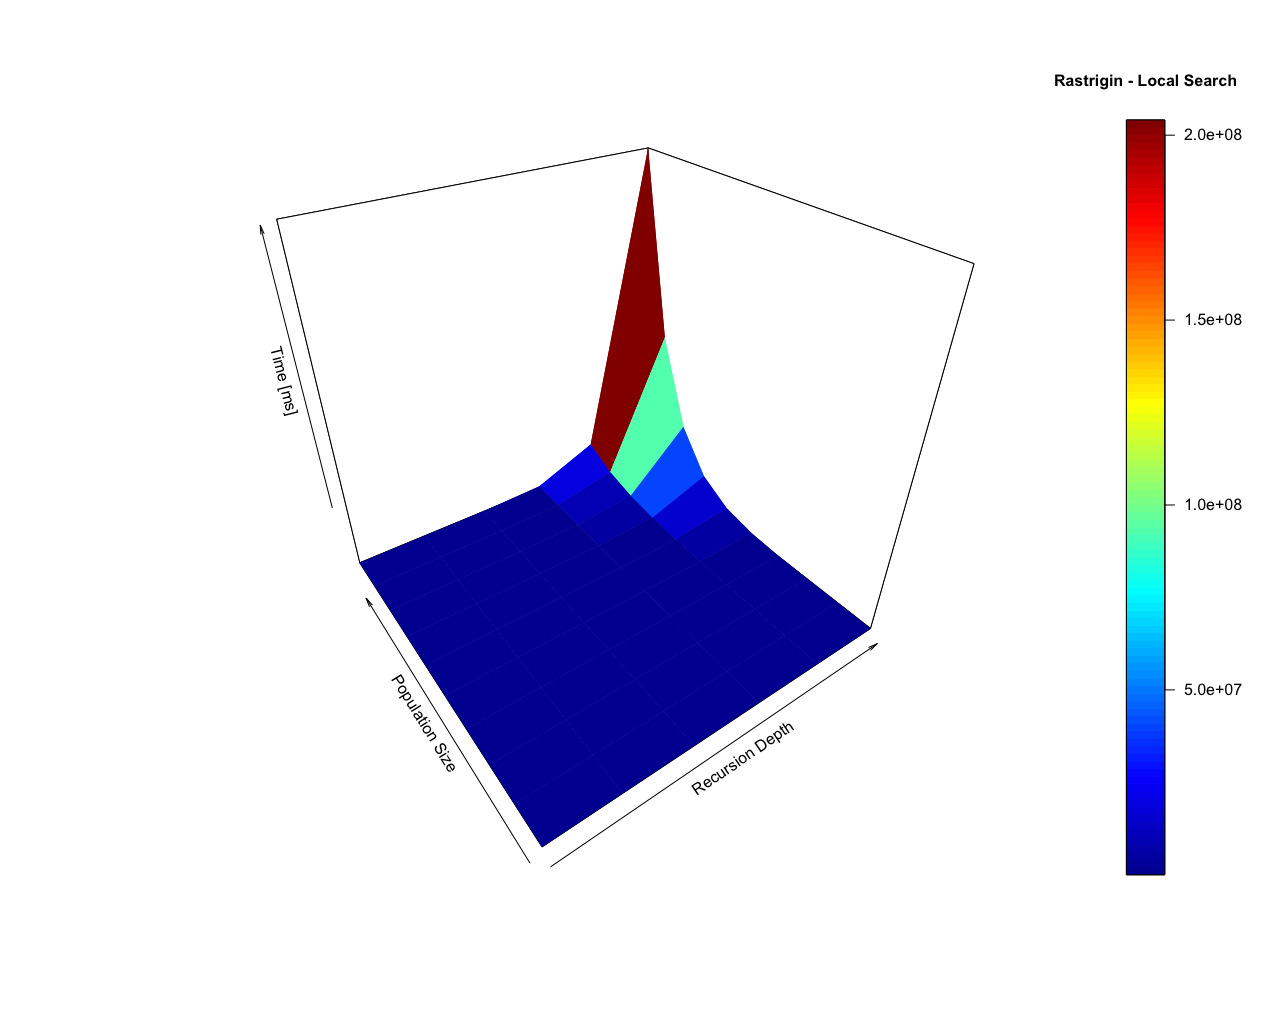
\includegraphics[width=0.8\linewidth]{fig0028.png}
%  \caption{Изчислително време [ms] за функцията Rastrigin с локално търсене}
%\label{fig0028}
%\end{figure}
%
%\begin{figure}[H]
%  \centering
%  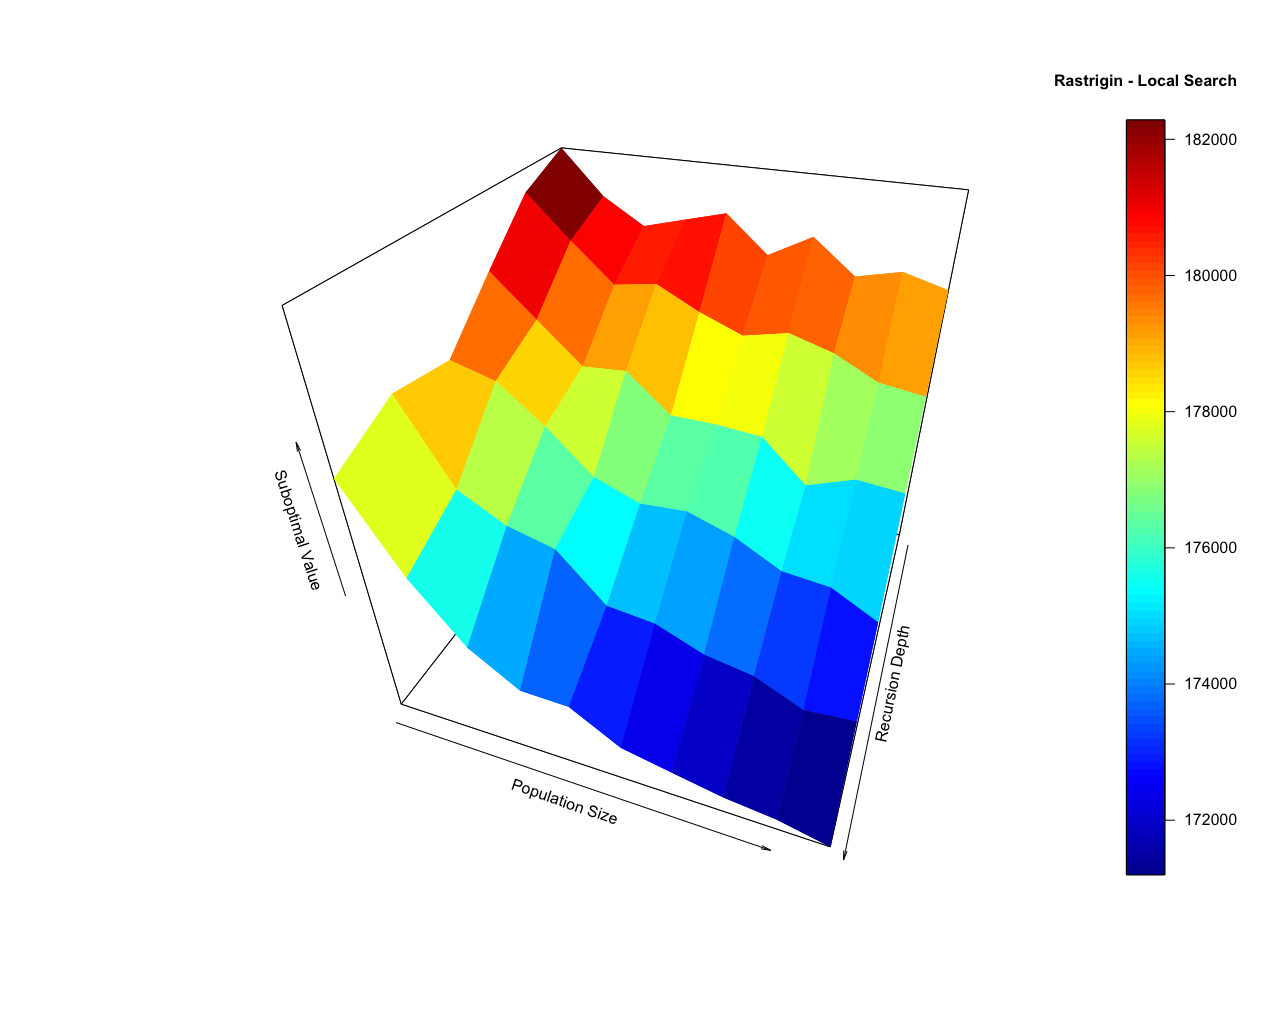
\includegraphics[width=0.8\linewidth]{fig0029.png}
%  \caption{Субоптимални стойности за функцията Rastrigin с локално търсене}
%\label{fig0029}
%\end{figure}
%
%\begin{figure}[H]
%  \centering
%  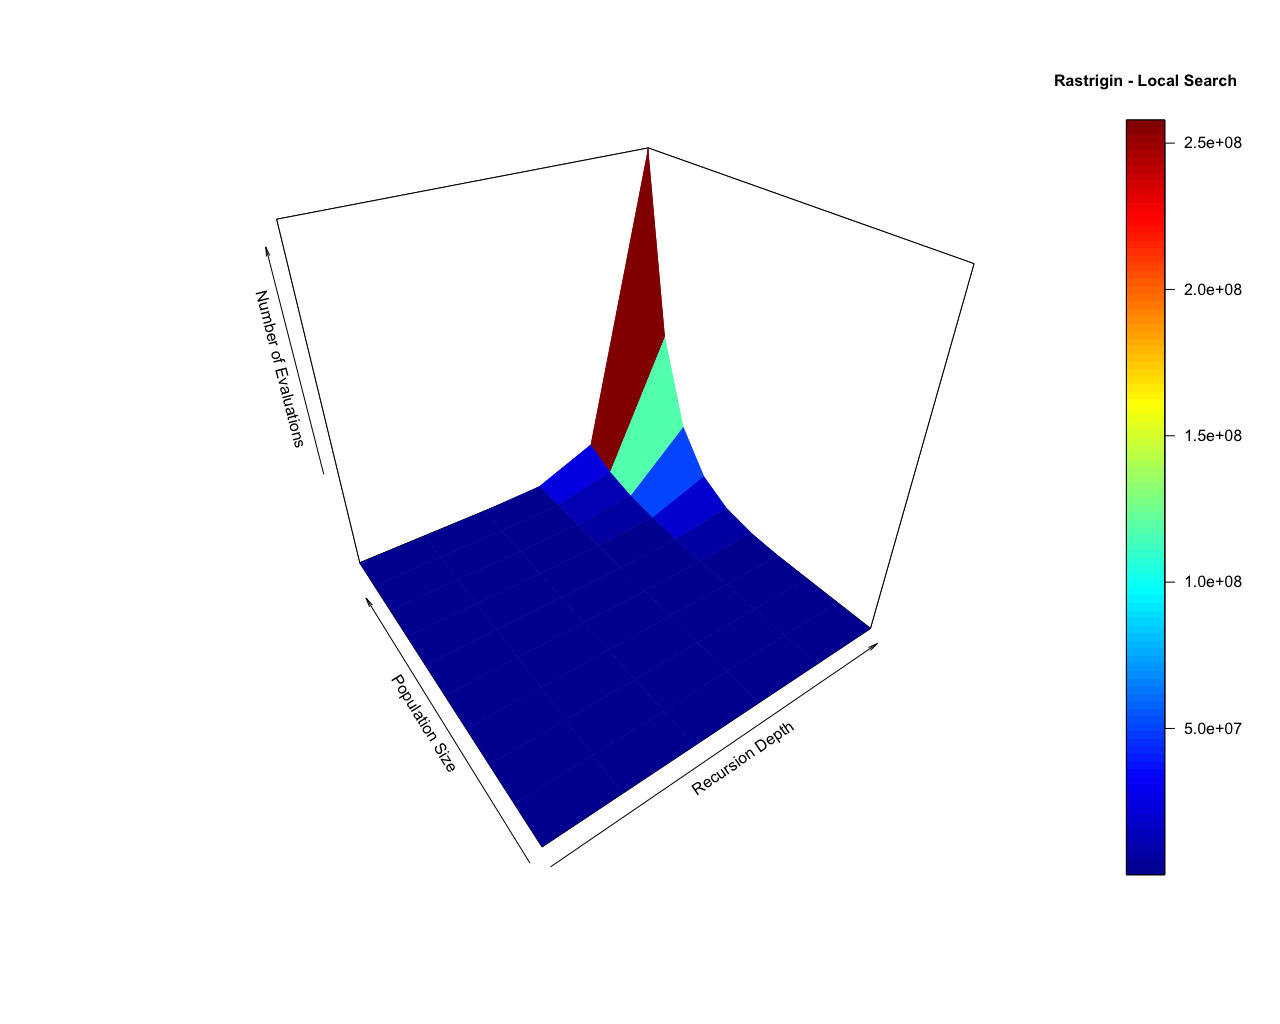
\includegraphics[width=0.8\linewidth]{fig0030.png}
%  \caption{Брой изчисления на функцията Rastrigin с локално търсене}
%\label{fig0030}
%\end{figure}
%
%
%\begin{figure}[H]
%  \centering
%  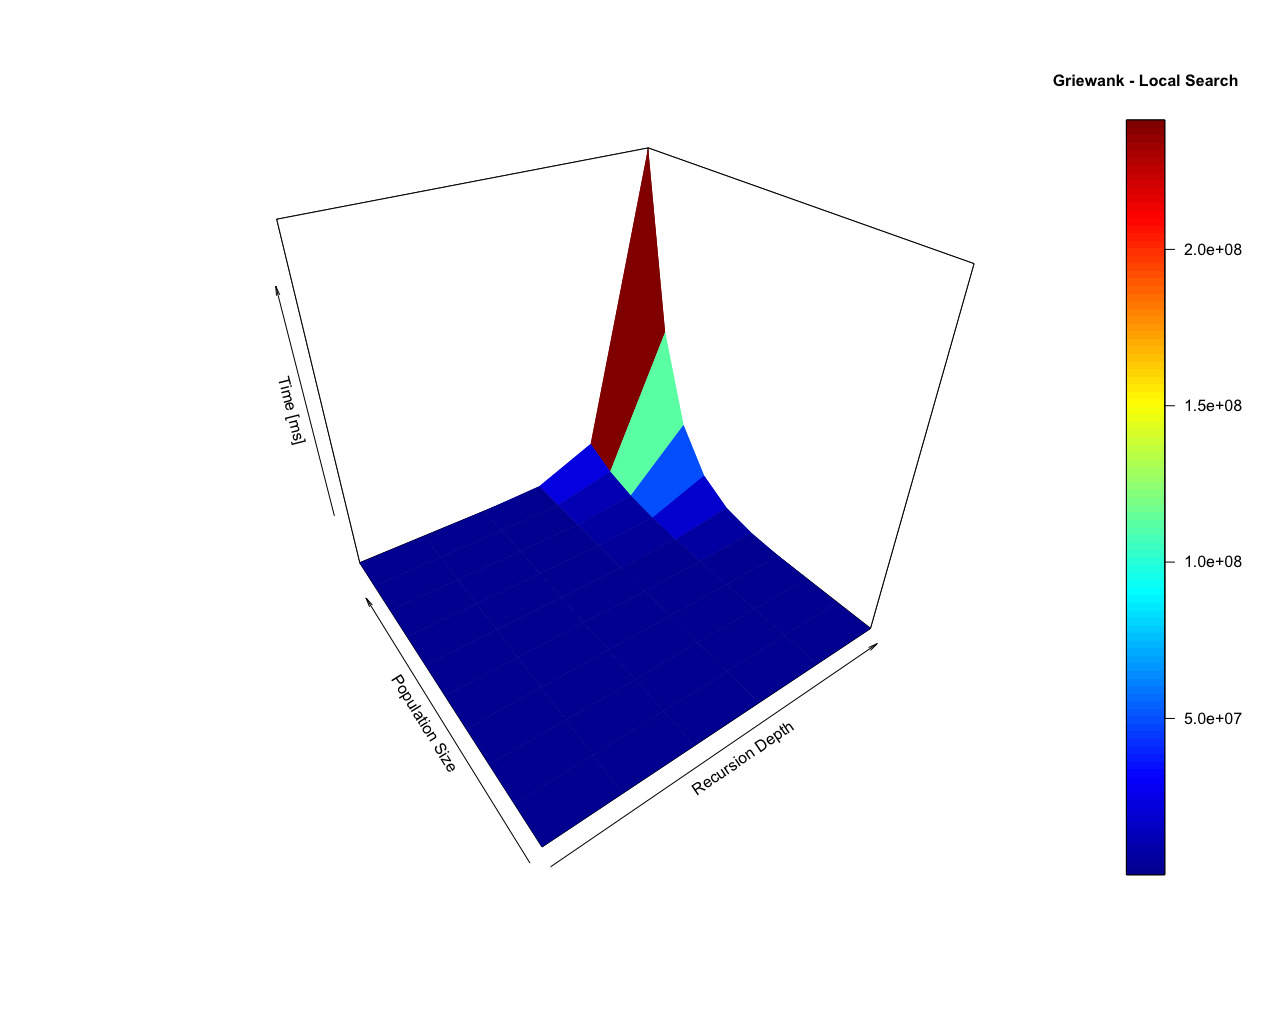
\includegraphics[width=0.8\linewidth]{fig0031.png}
%  \caption{Изчислително време [ms] за функцията Griewank с локално търсене}
%\label{fig0031}
%\end{figure}
%
%\begin{figure}[H]
%  \centering
%  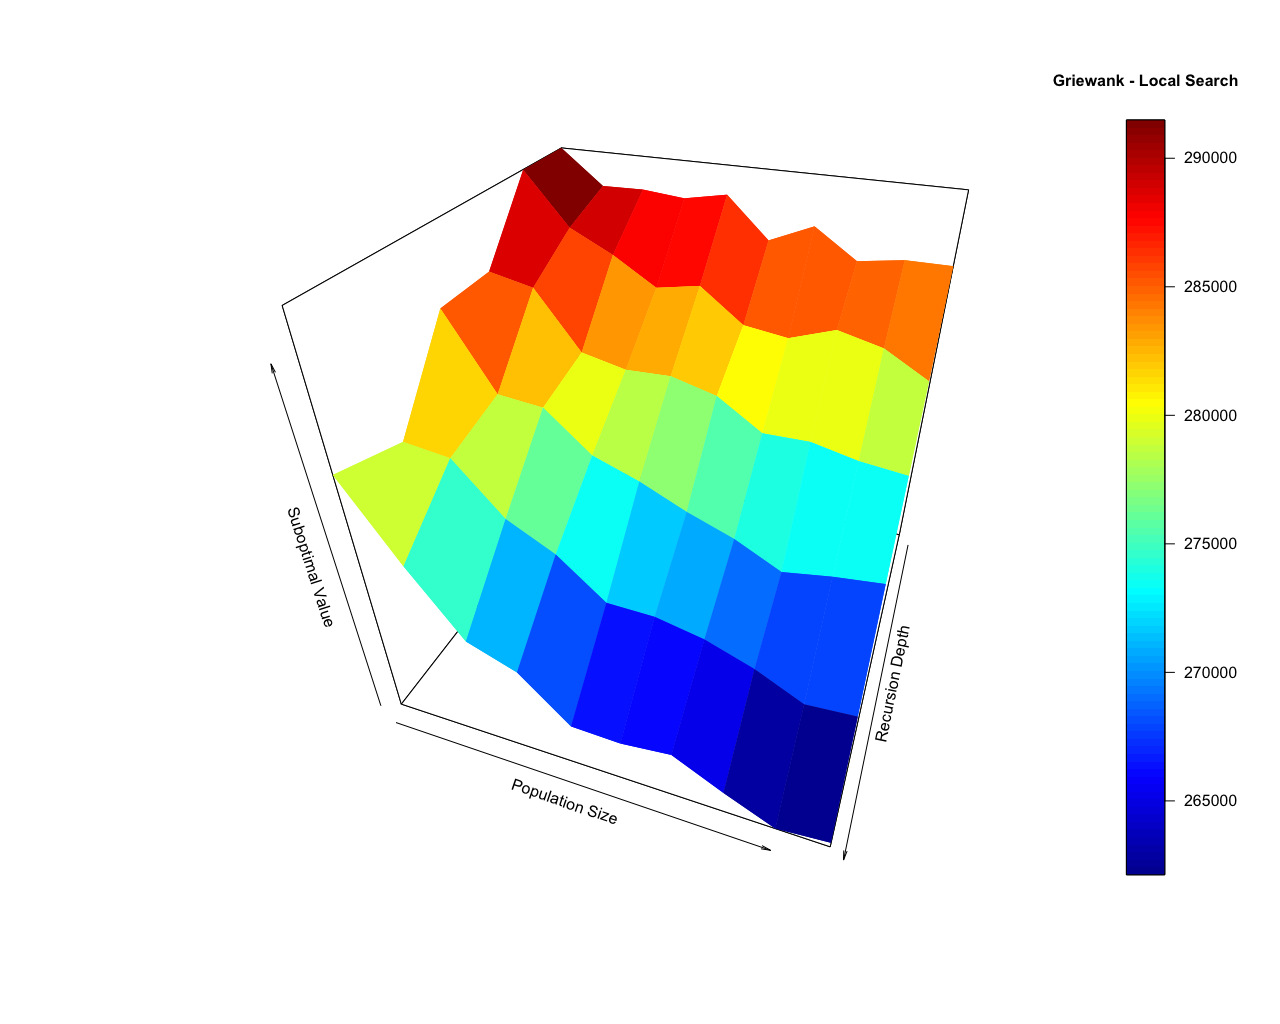
\includegraphics[width=0.8\linewidth]{fig0032.png}
%  \caption{Субоптимални стойности за функцията Griewank с локално търсене}
%\label{fig0032}
%\end{figure}
%
%\begin{figure}[H]
%  \centering
%  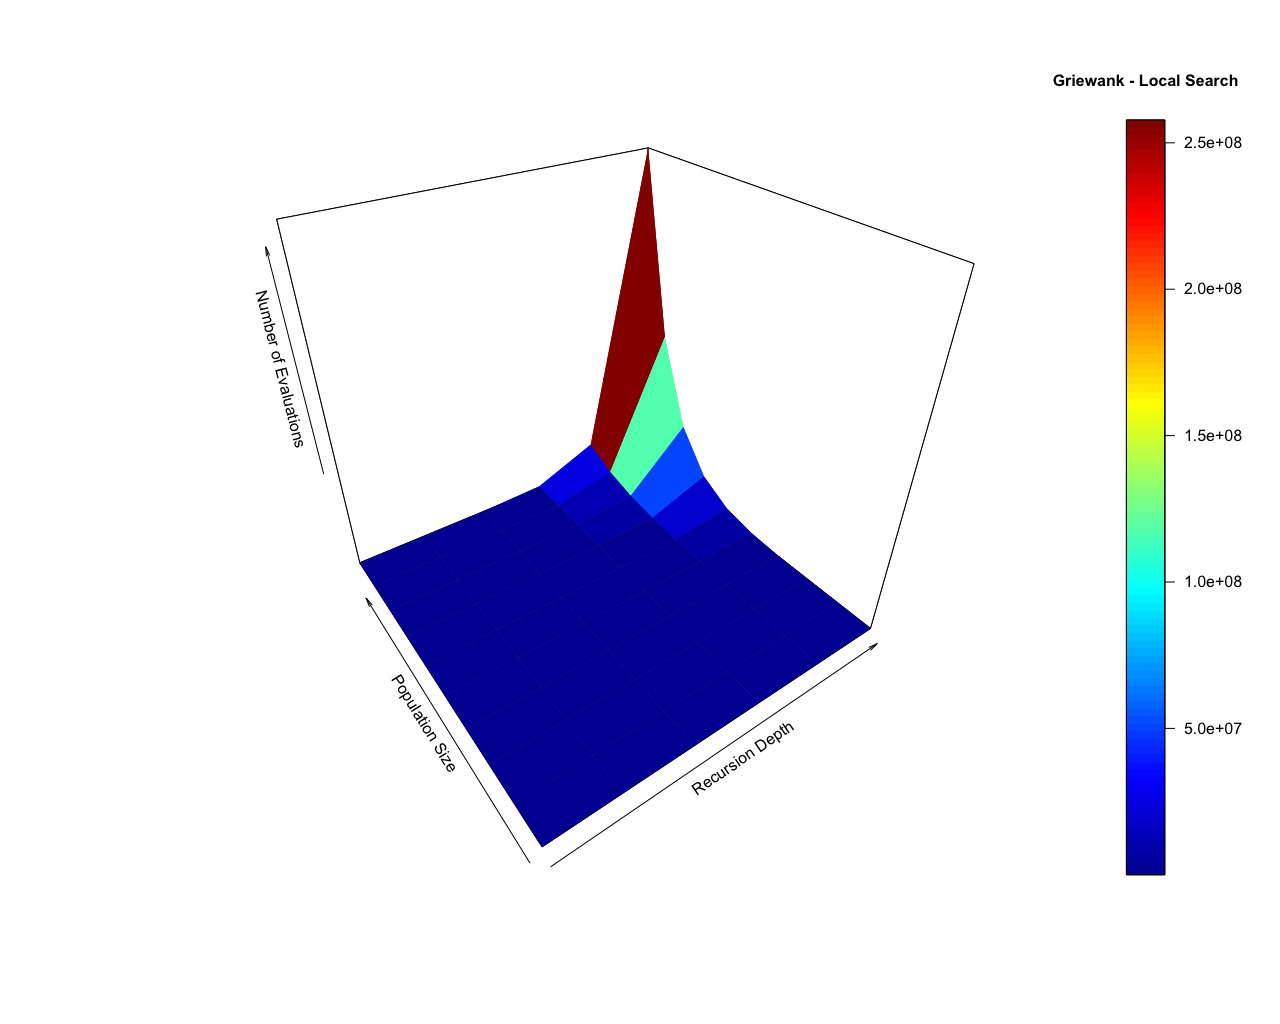
\includegraphics[width=0.8\linewidth]{fig0033.png}
%  \caption{Брой изчисления на функцията Griewank с локално търсене}
%\label{fig0033}
%\end{figure}
%
%\begin{figure}[H]
%  \centering
%  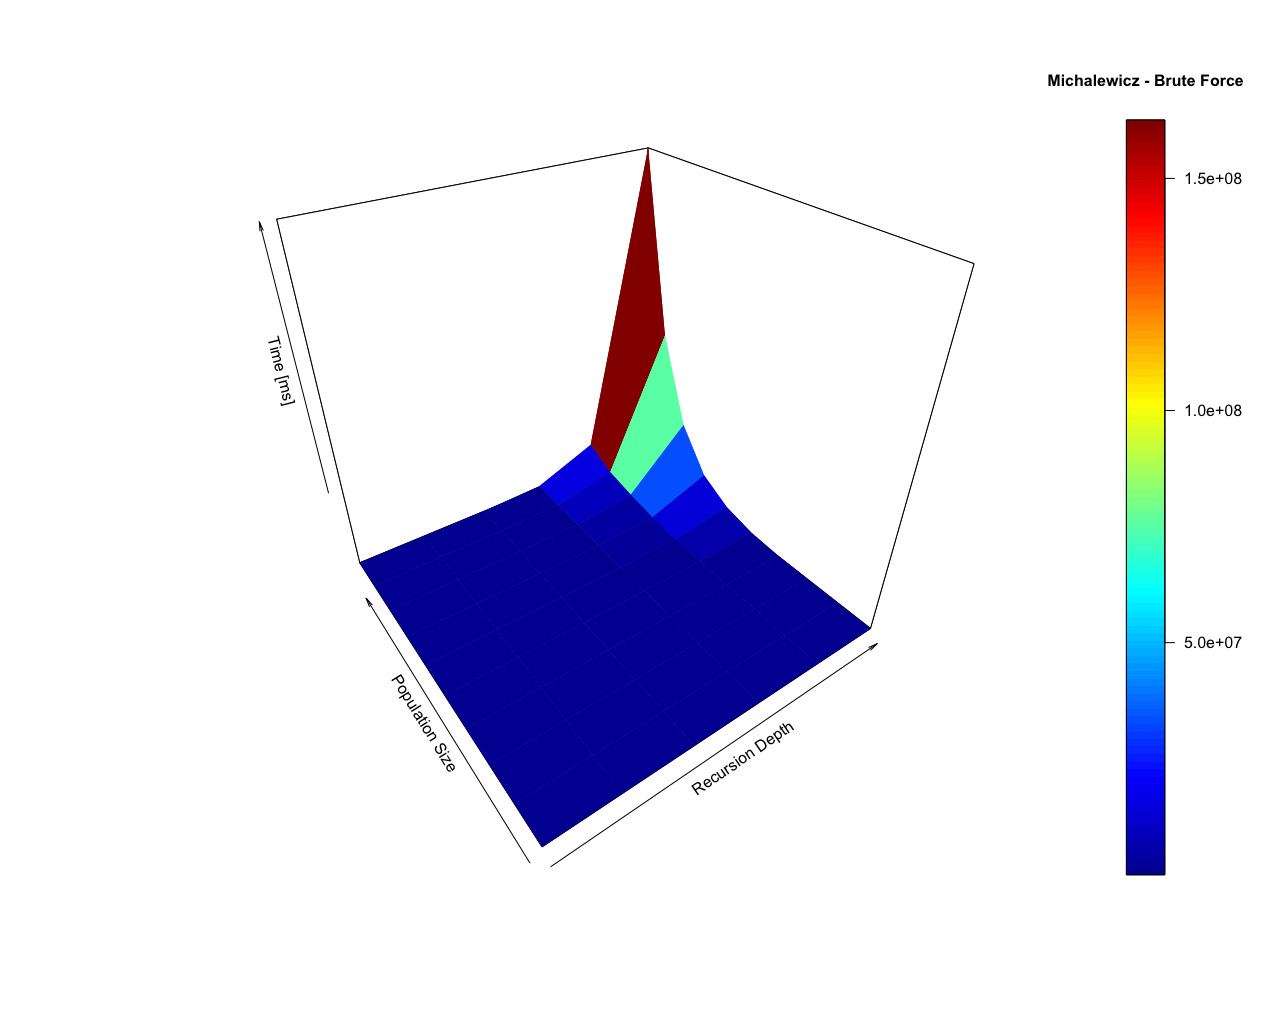
\includegraphics[width=0.8\linewidth]{fig0034.png}
%  \caption{Изчислително време [ms] за функцията Michalewicz с пълно изчерпване}
%\label{fig0034}
%\end{figure}
%
%\begin{figure}[H]
%  \centering
%  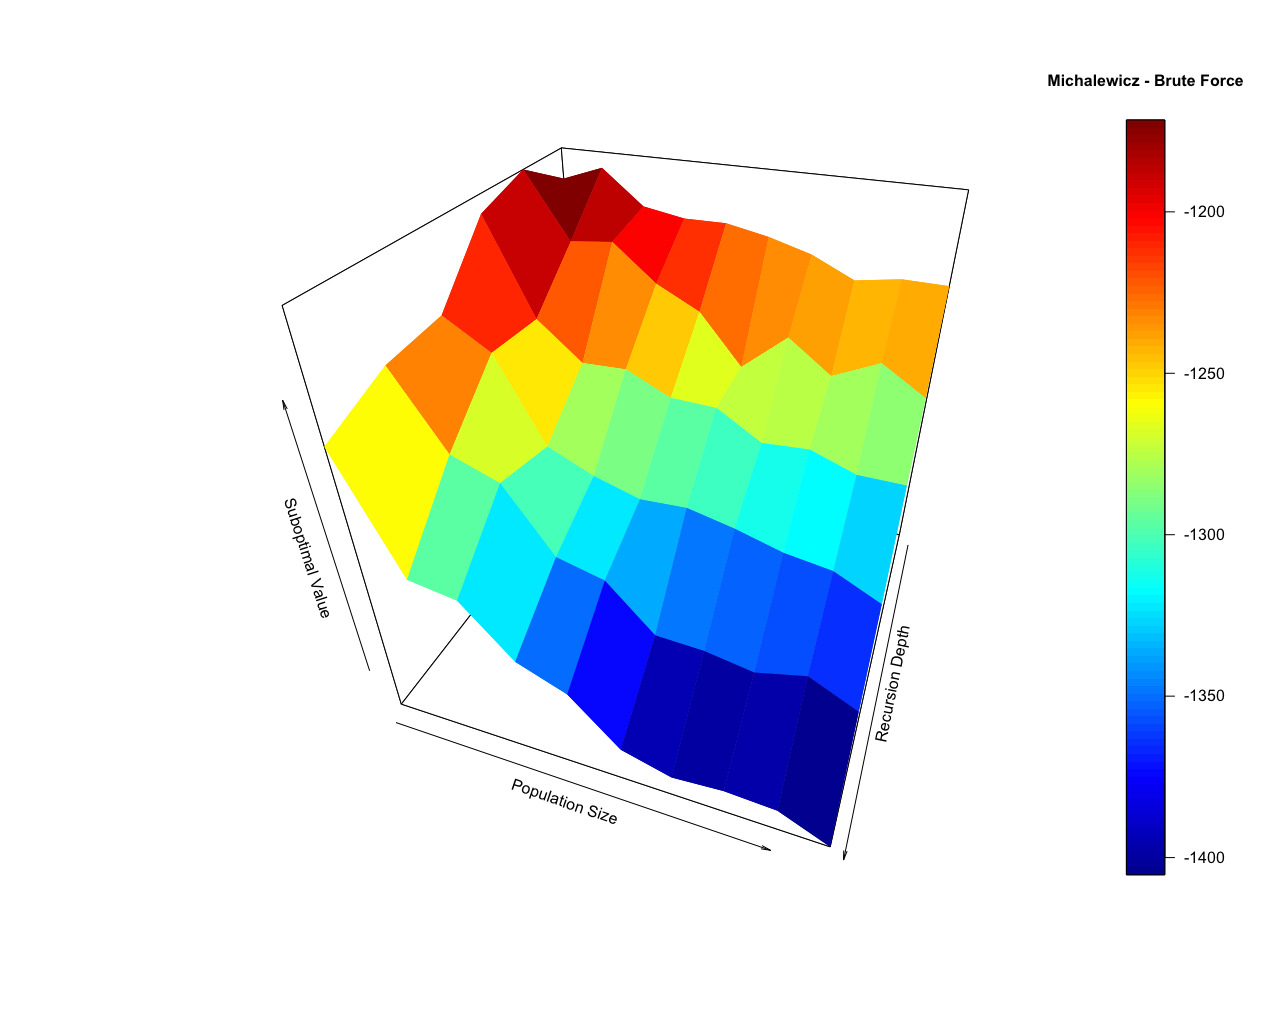
\includegraphics[width=0.8\linewidth]{fig0035.png}
%  \caption{Субоптимални стойности за функцията Michalewicz с пълно изчерпване}
%\label{fig0035}
%\end{figure}
%
%\begin{figure}[H]
%  \centering
%  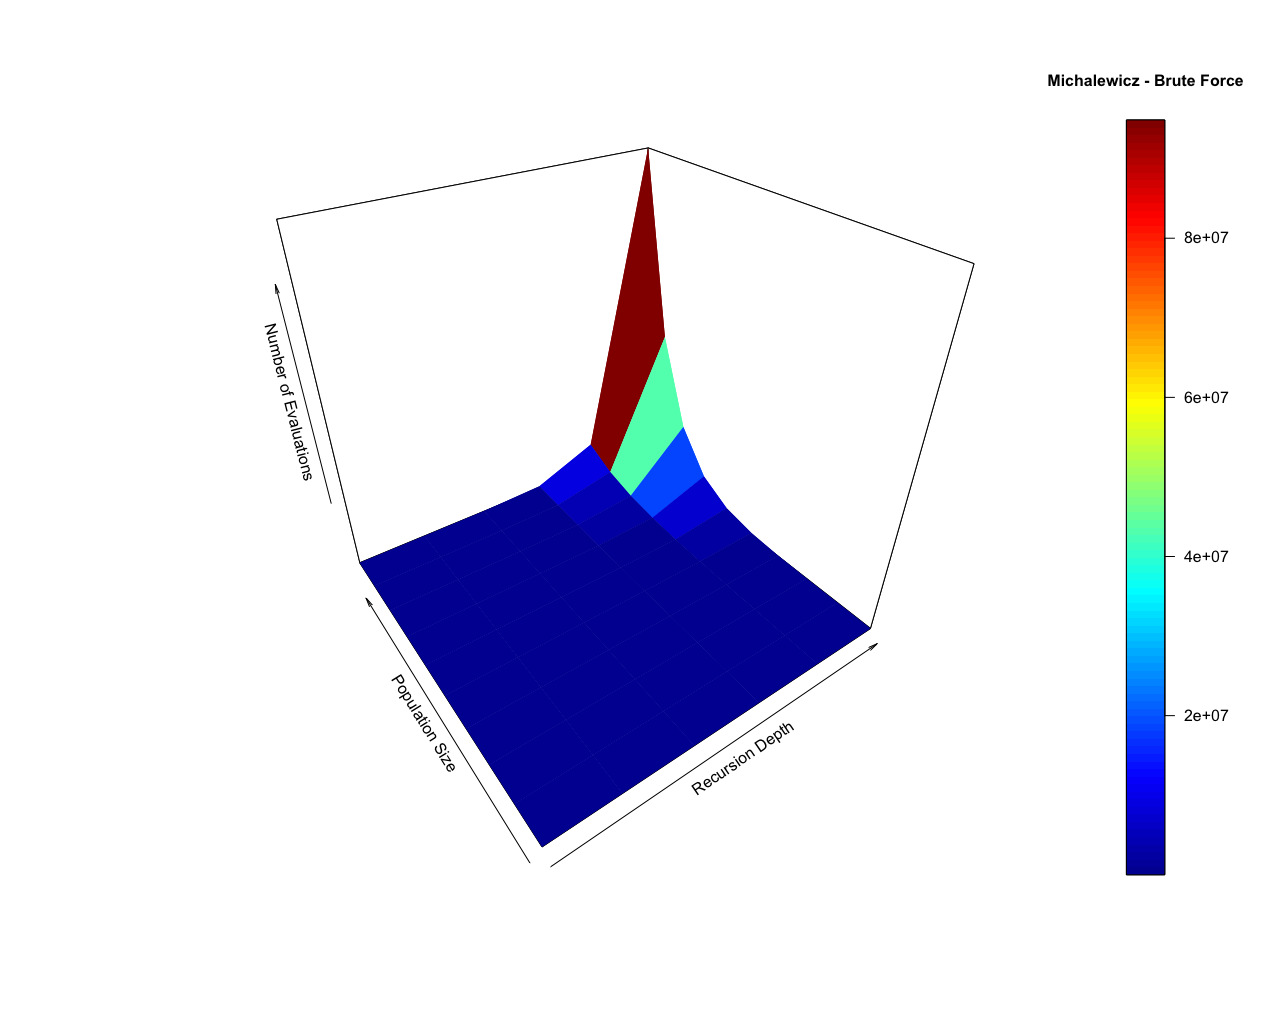
\includegraphics[width=0.8\linewidth]{fig0036.png}
%  \caption{Брой изчисления на функцията Michalewicz с пълно изчерпване}
%\label{fig0036}
%\end{figure}
%
%\begin{figure}[H]
%  \centering
%  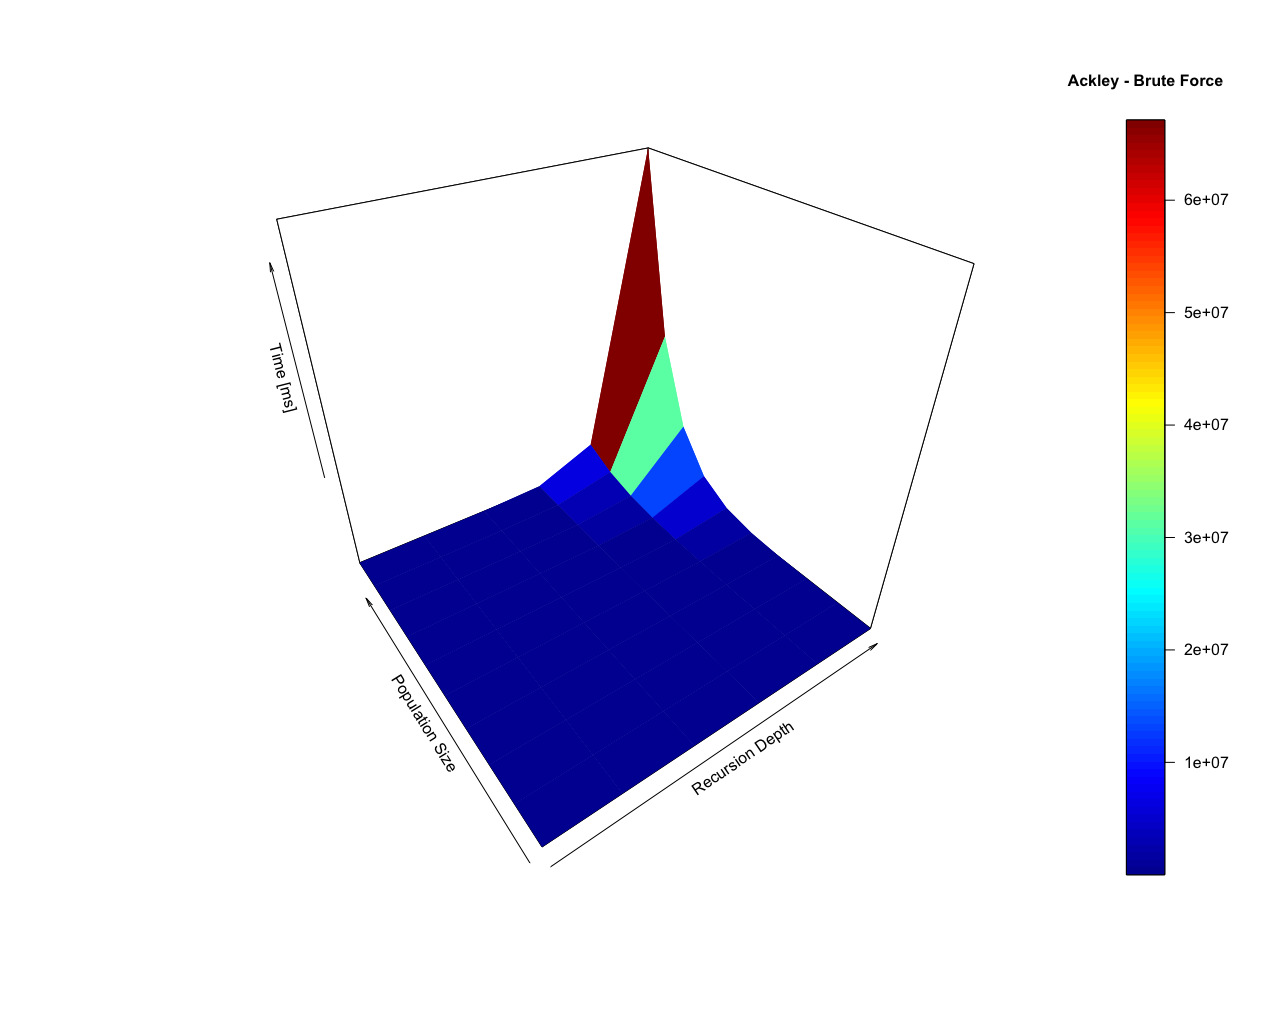
\includegraphics[width=0.8\linewidth]{fig0037.png}
%  \caption{Изчислително време [ms] за функцията Ackley с пълно изчерпване}
%\label{fig0037}
%\end{figure}
%
%\begin{figure}[H]
%  \centering
%  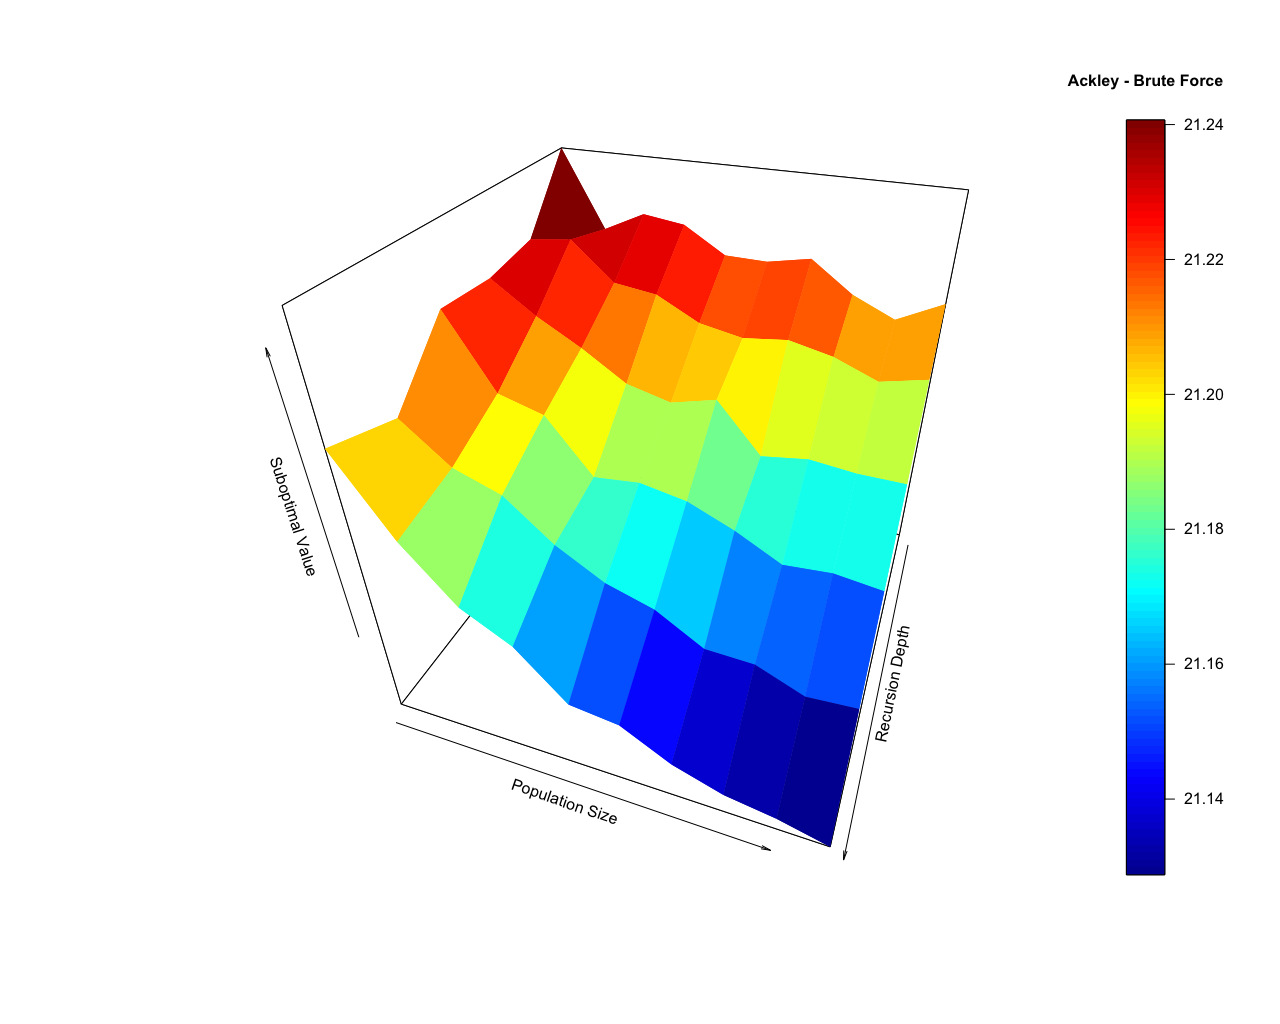
\includegraphics[width=0.8\linewidth]{fig0038.png}
%  \caption{Субоптимални стойности за функцията Ackley с пълно изчерпване}
%\label{fig0038}
%\end{figure}
%
%\begin{figure}[H]
%  \centering
%  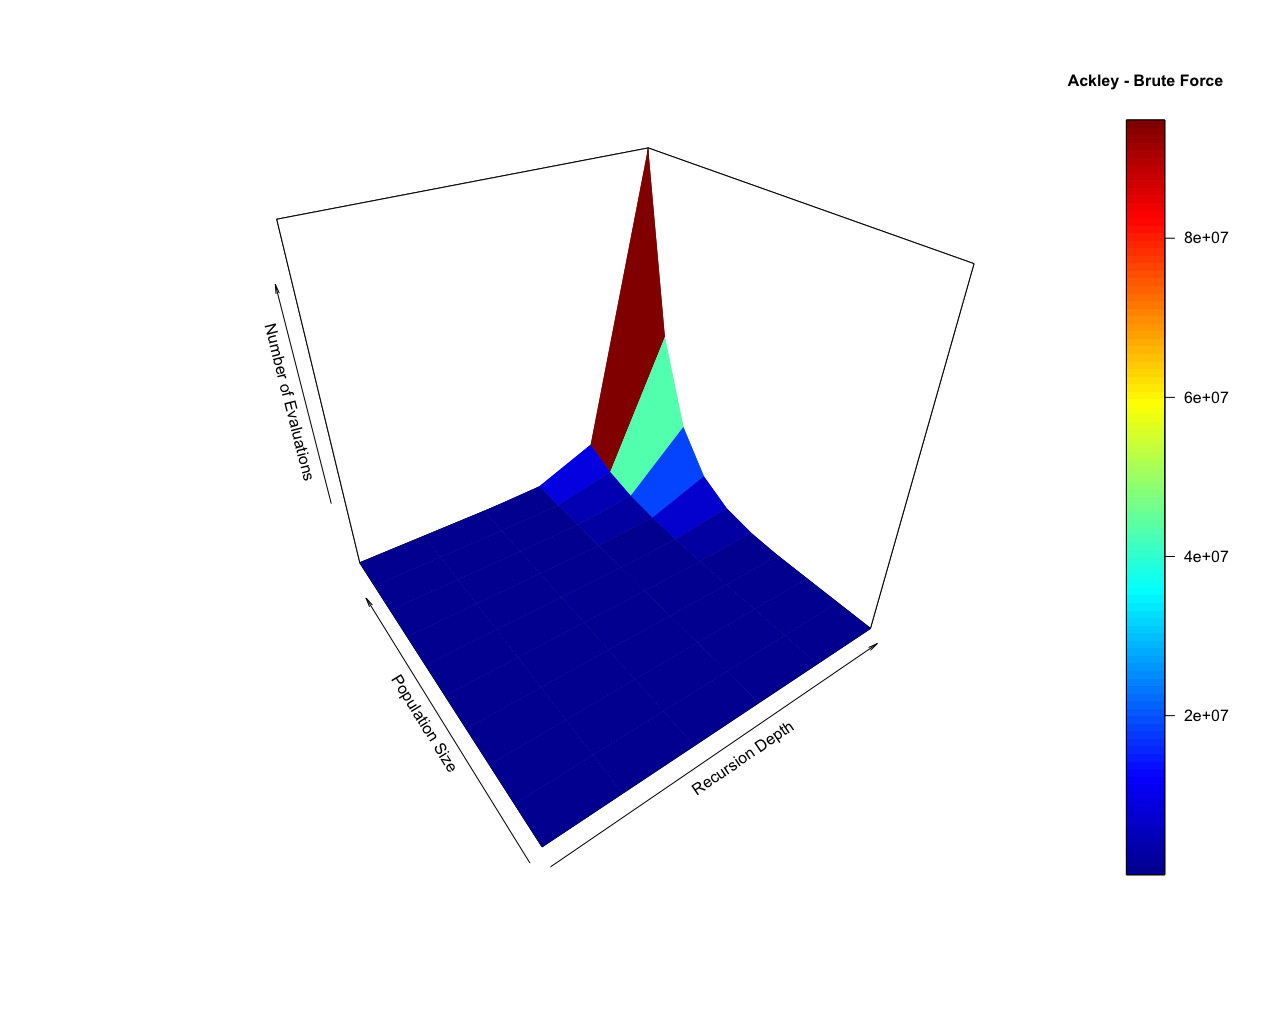
\includegraphics[width=0.8\linewidth]{fig0039.png}
%  \caption{Брой изчисления на функцията Ackley с пълно изчерпване}
%\label{fig0039}
%\end{figure}
%
%\begin{figure}[H]
%  \centering
%  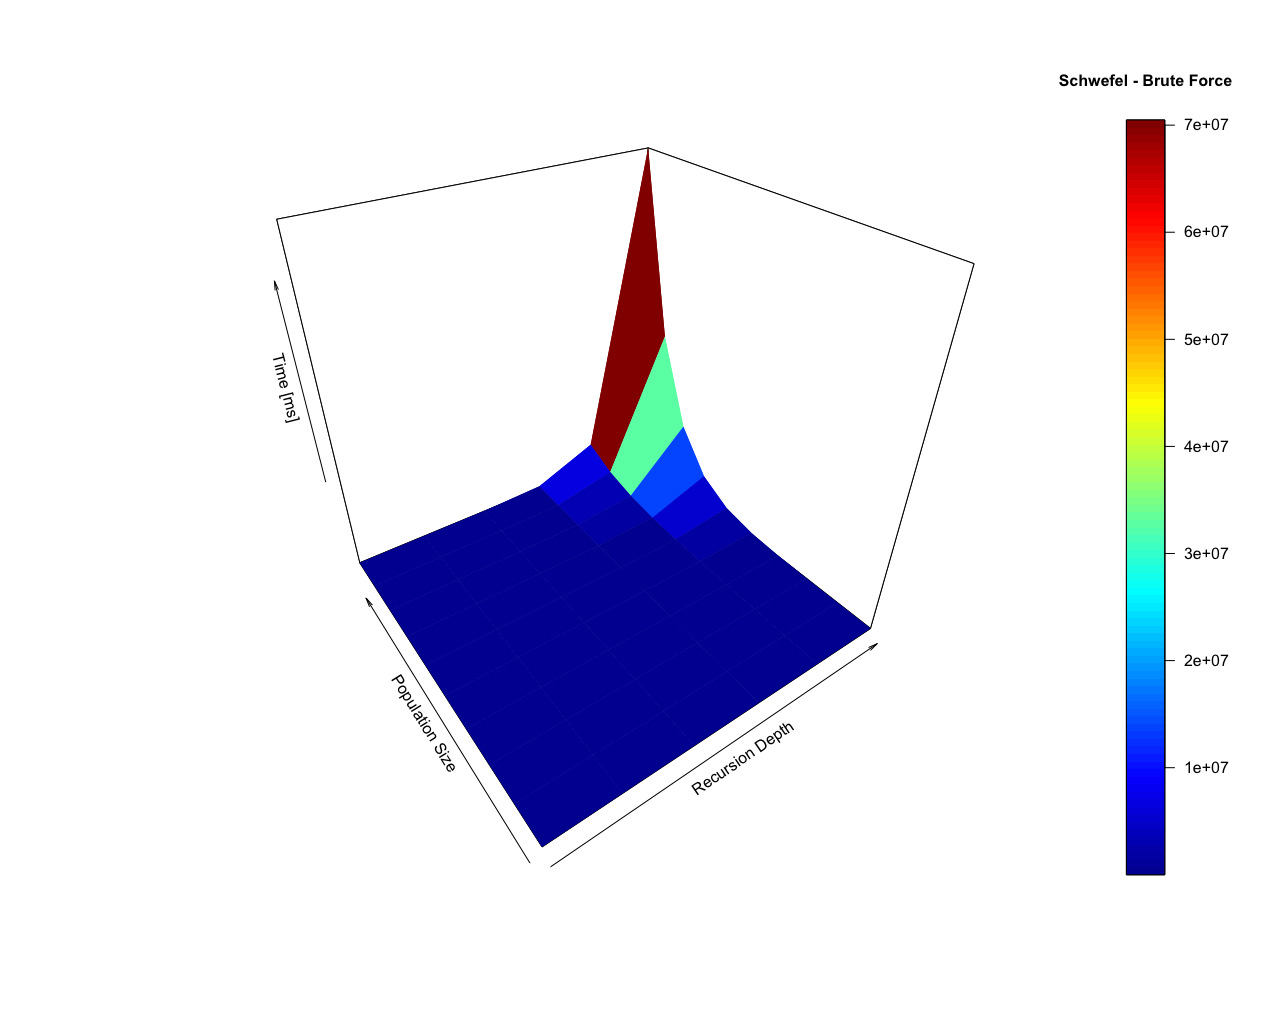
\includegraphics[width=0.8\linewidth]{fig0040.png}
%  \caption{Изчислително време [ms] за функцията Schwefel с пълно изчерпване}
%\label{fig0040}
%\end{figure}
%
%\begin{figure}[H]
%  \centering
%  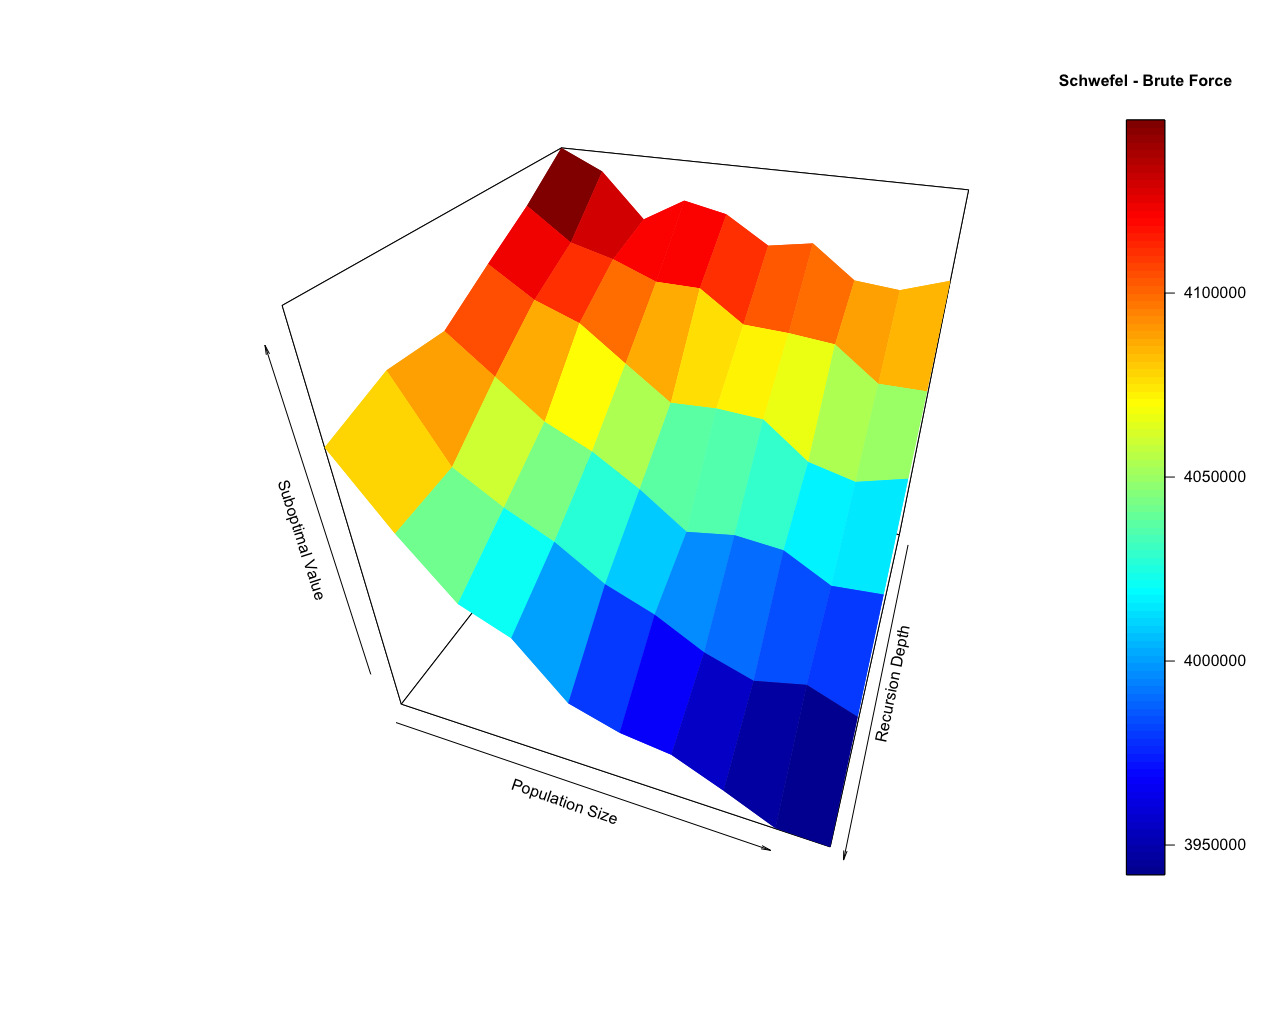
\includegraphics[width=0.8\linewidth]{fig0041.png}
%  \caption{Субоптимални стойности за функцията Schwefel с пълно изчерпване}
%\label{fig0041}
%\end{figure}
%
%\begin{figure}[H]
%  \centering
%  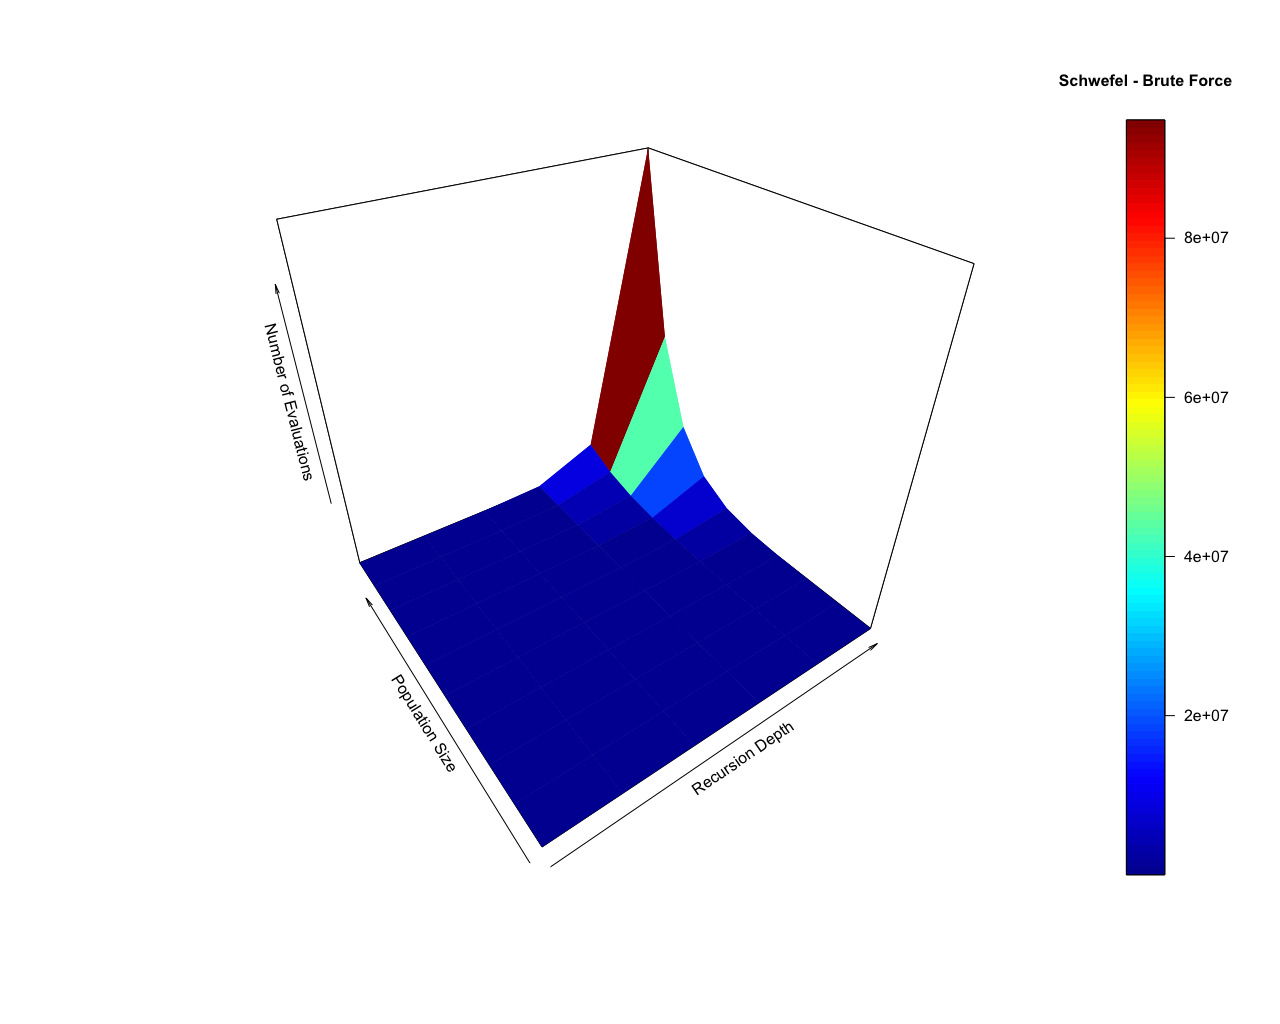
\includegraphics[width=0.8\linewidth]{fig0042.png}
%  \caption{Брой изчисления на функцията Schwefel с пълно изчерпване}
%\label{fig0042}
%\end{figure}
%
%\begin{figure}[H]
%  \centering
%  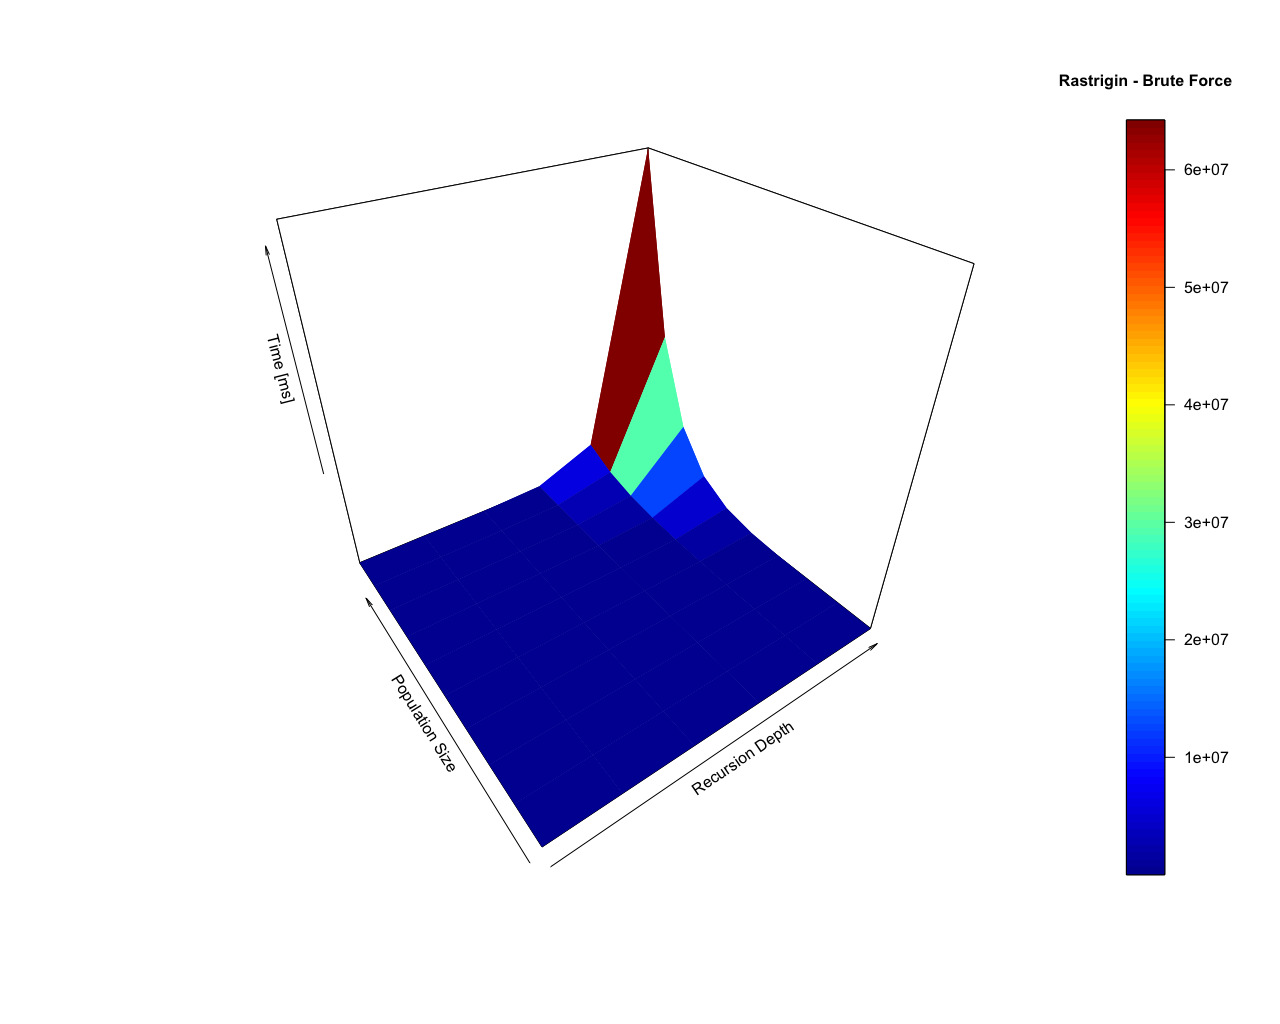
\includegraphics[width=0.8\linewidth]{fig0043.png}
%  \caption{Изчислително време [ms] за функцията Rastrigin с пълно изчерпване}
%\label{fig0043}
%\end{figure}
%
%\begin{figure}[H]
%  \centering
%  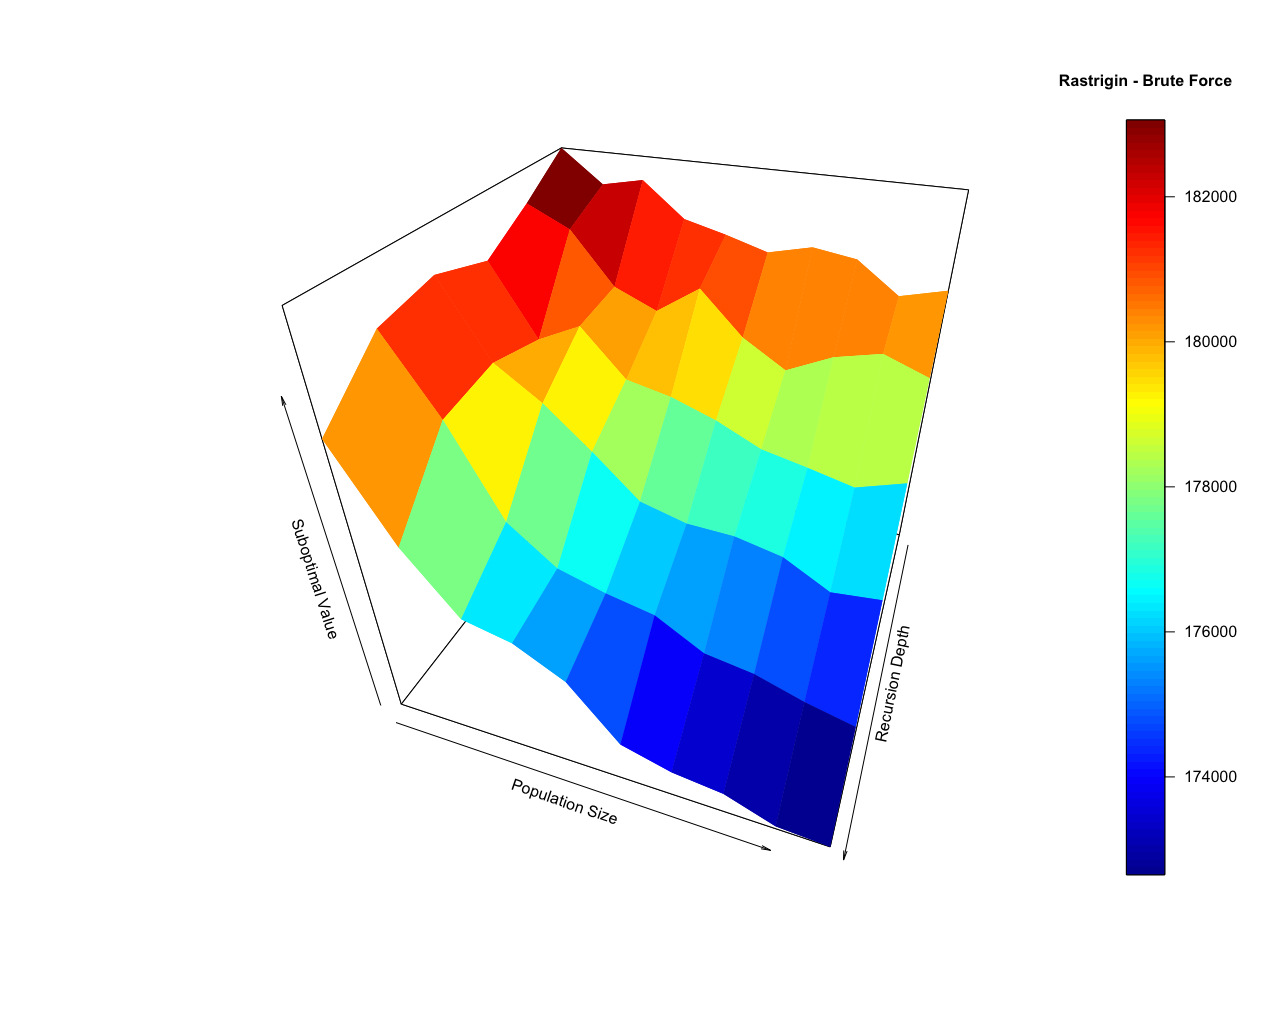
\includegraphics[width=0.8\linewidth]{fig0044.png}
%  \caption{Субоптимални стойности за функцията Rastrigin с пълно изчерпване}
%\label{fig0044}
%\end{figure}
%
%\begin{figure}[H]
%  \centering
%  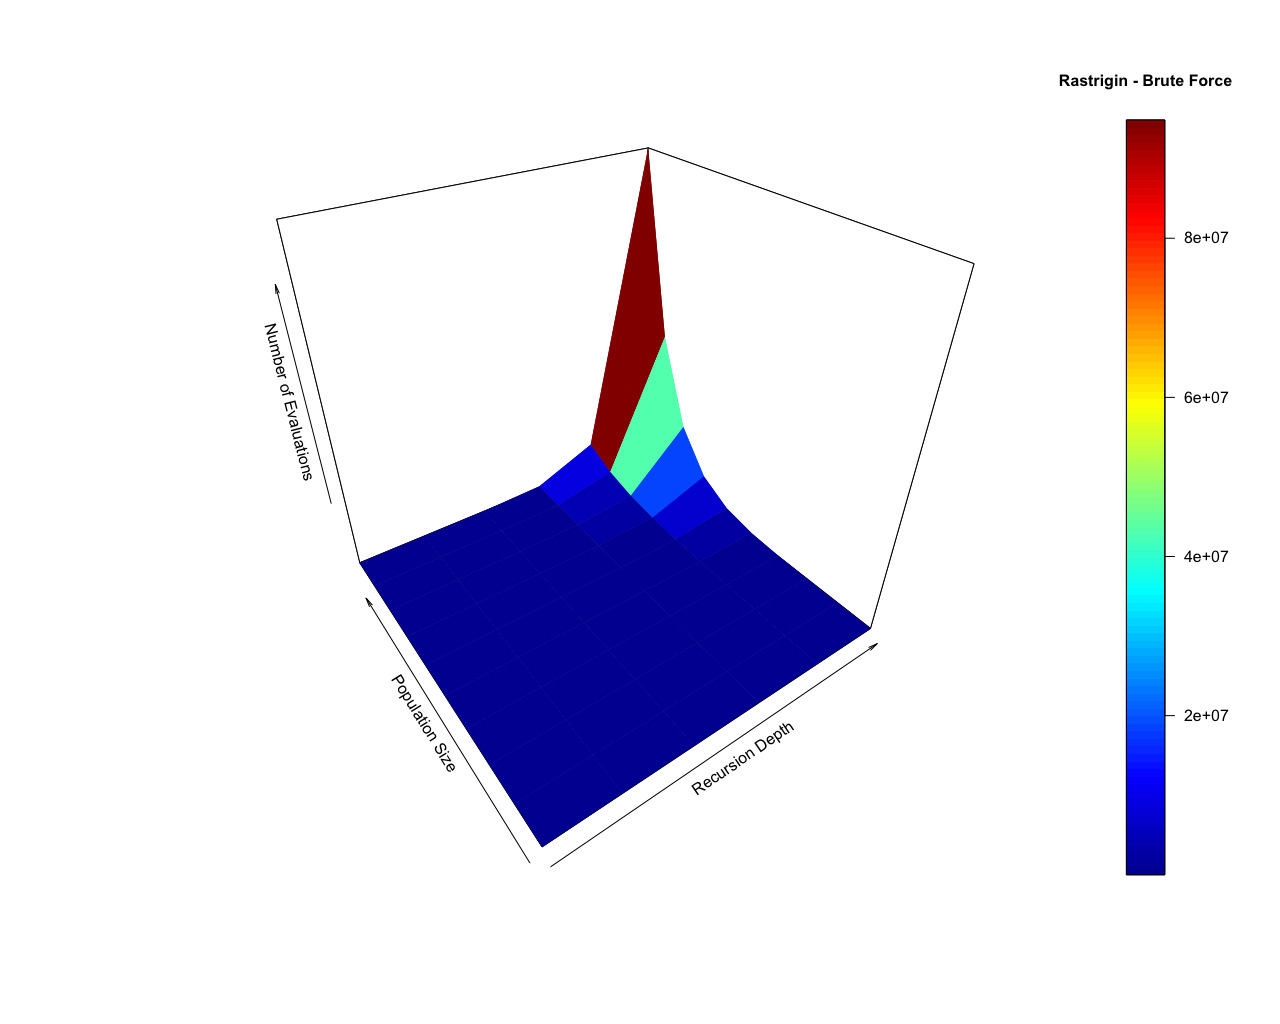
\includegraphics[width=0.8\linewidth]{fig0045.png}
%  \caption{Брой изчисления на функцията Rastrigin с пълно изчерпване}
%\label{fig0045}
%\end{figure}
%
%\begin{figure}[H]
%  \centering
%  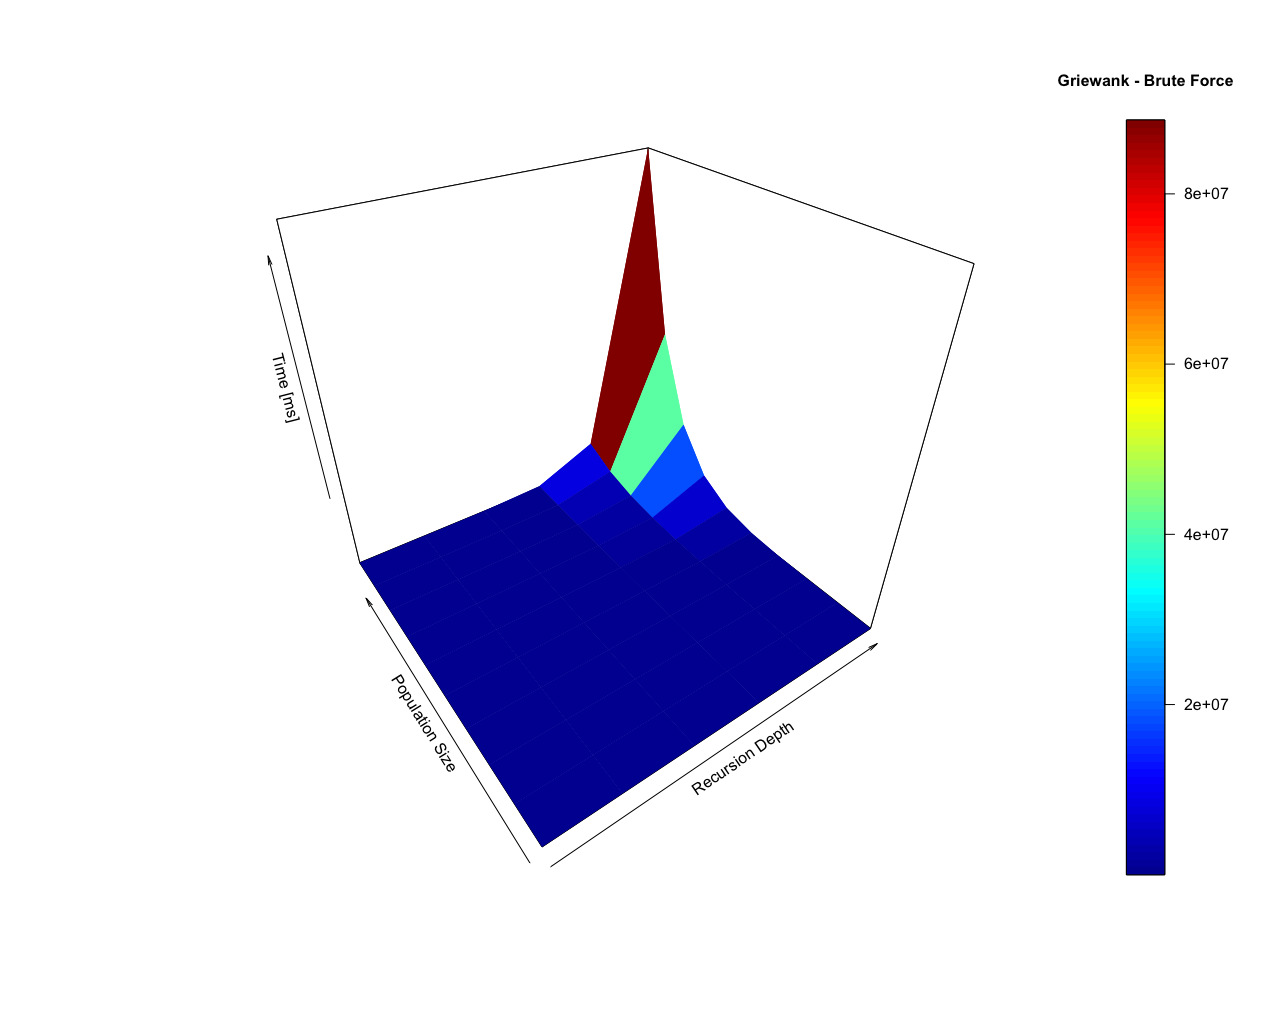
\includegraphics[width=0.8\linewidth]{fig0046.png}
%  \caption{Изчислително време [ms] за функцията Griewank с пълно изчерпване}
%\label{fig0046}
%\end{figure}
%
%\begin{figure}[H]
%  \centering
%  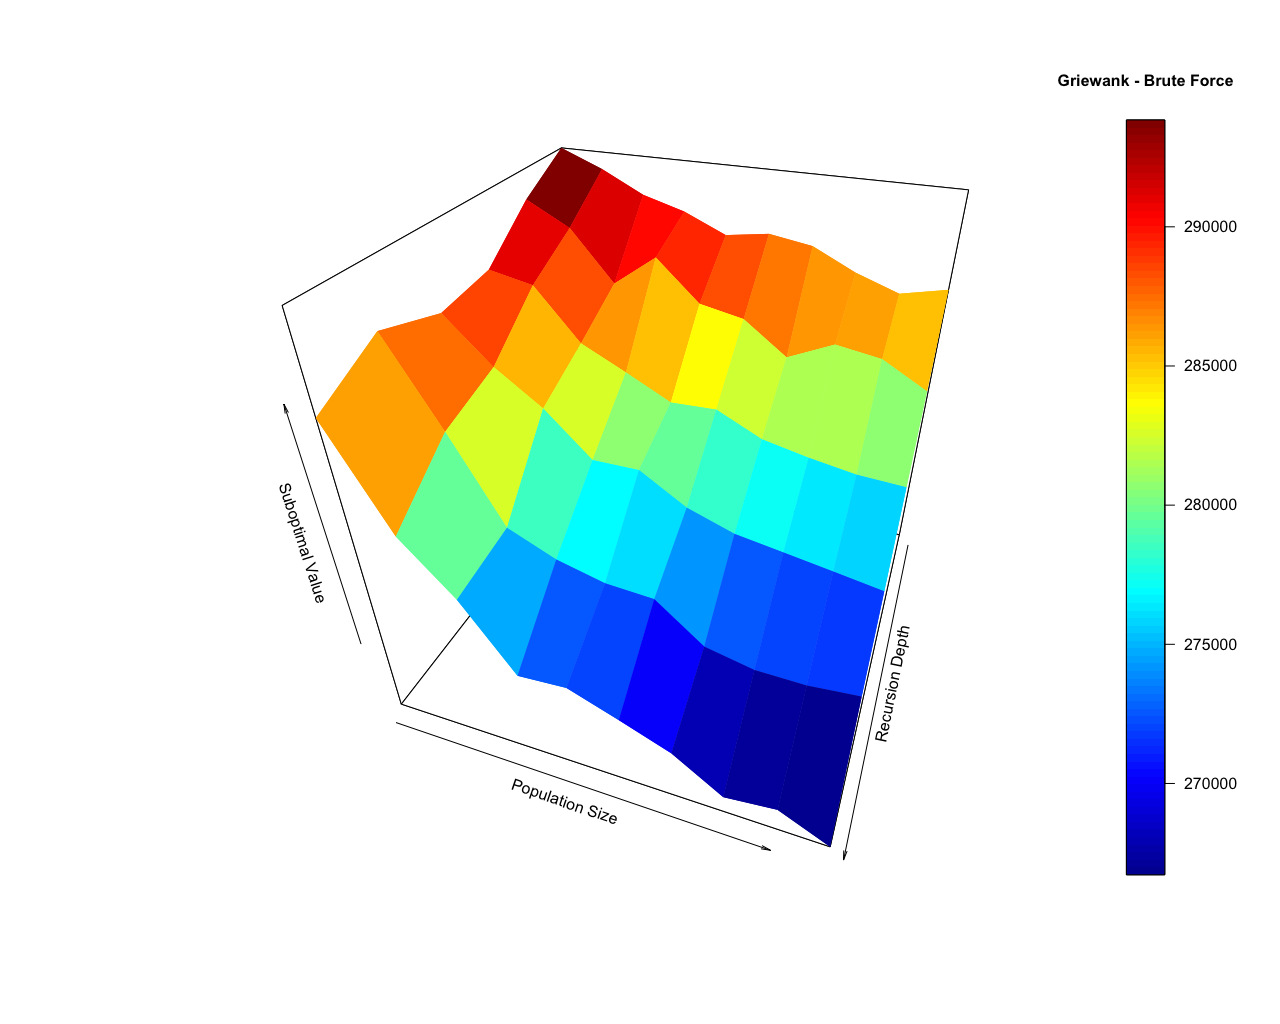
\includegraphics[width=0.8\linewidth]{fig0047.png}
%  \caption{Субоптимални стойности за функцията Griewank с пълно изчерпване}
%\label{fig0047}
%\end{figure}
%
%\begin{figure}[H]
%  \centering
%  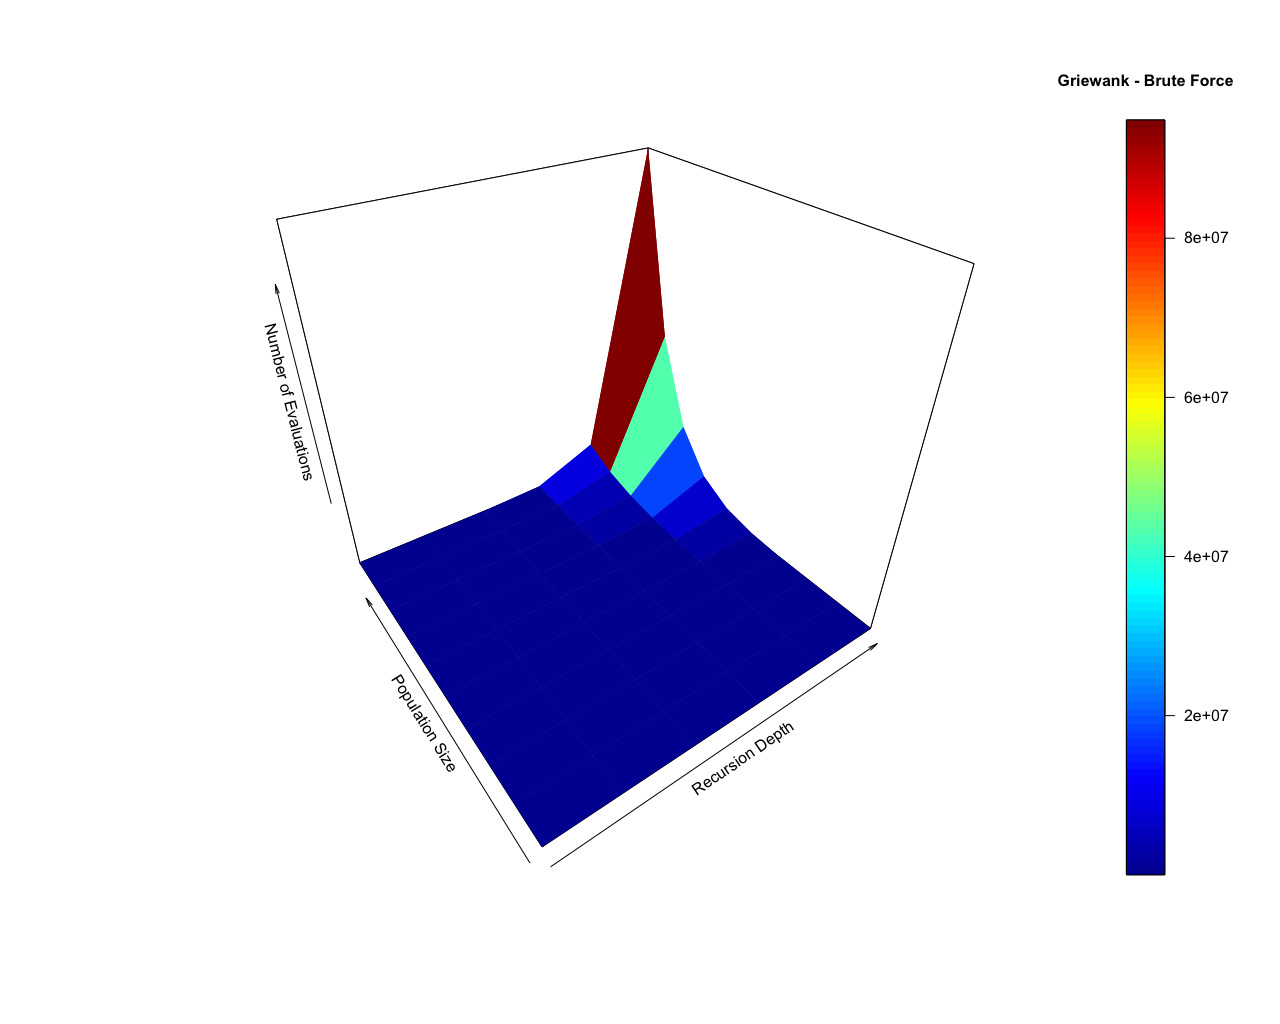
\includegraphics[width=0.8\linewidth]{fig0048.png}
%  \caption{Брой изчисления на функцията Griewank с пълно изчерпване}
%\label{fig0048}
%\end{figure}
%
\begin{figure}[H]
  \begin{subfigure}{0.31\textwidth}
  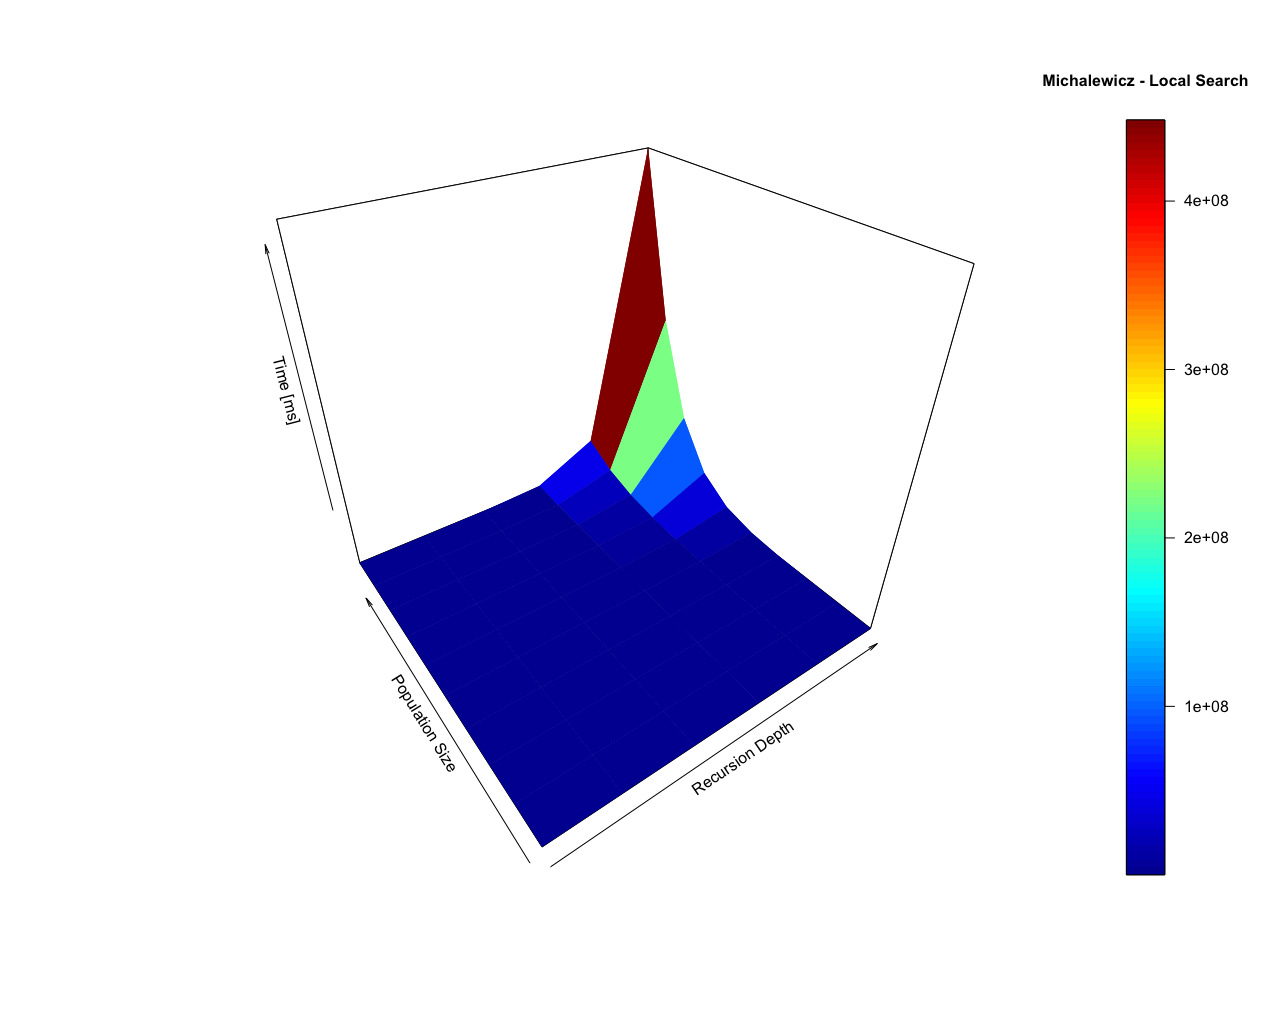
\includegraphics[width=\linewidth]{fig0019.png}
  \subcaption{\tiny Изчислително време [ms]}
  \label{fig0019}
  \end{subfigure}
  \begin{subfigure}{0.31\textwidth}
  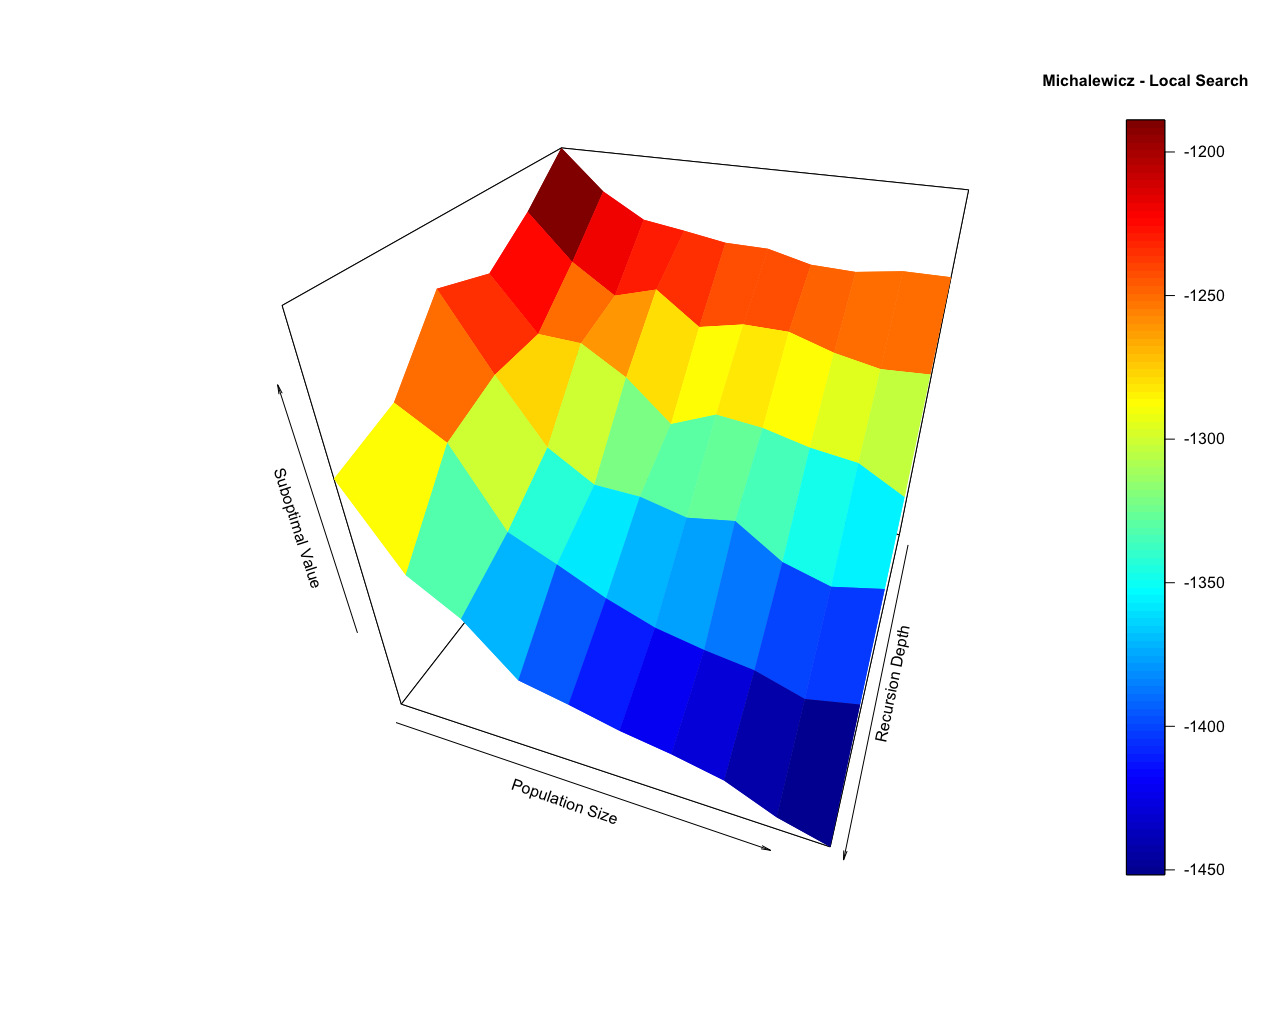
\includegraphics[width=\linewidth]{fig0020.png}
  \subcaption{\tiny Субоптимални стойности}
  \label{fig0020}
  \end{subfigure}
  \begin{subfigure}{0.31\textwidth}
  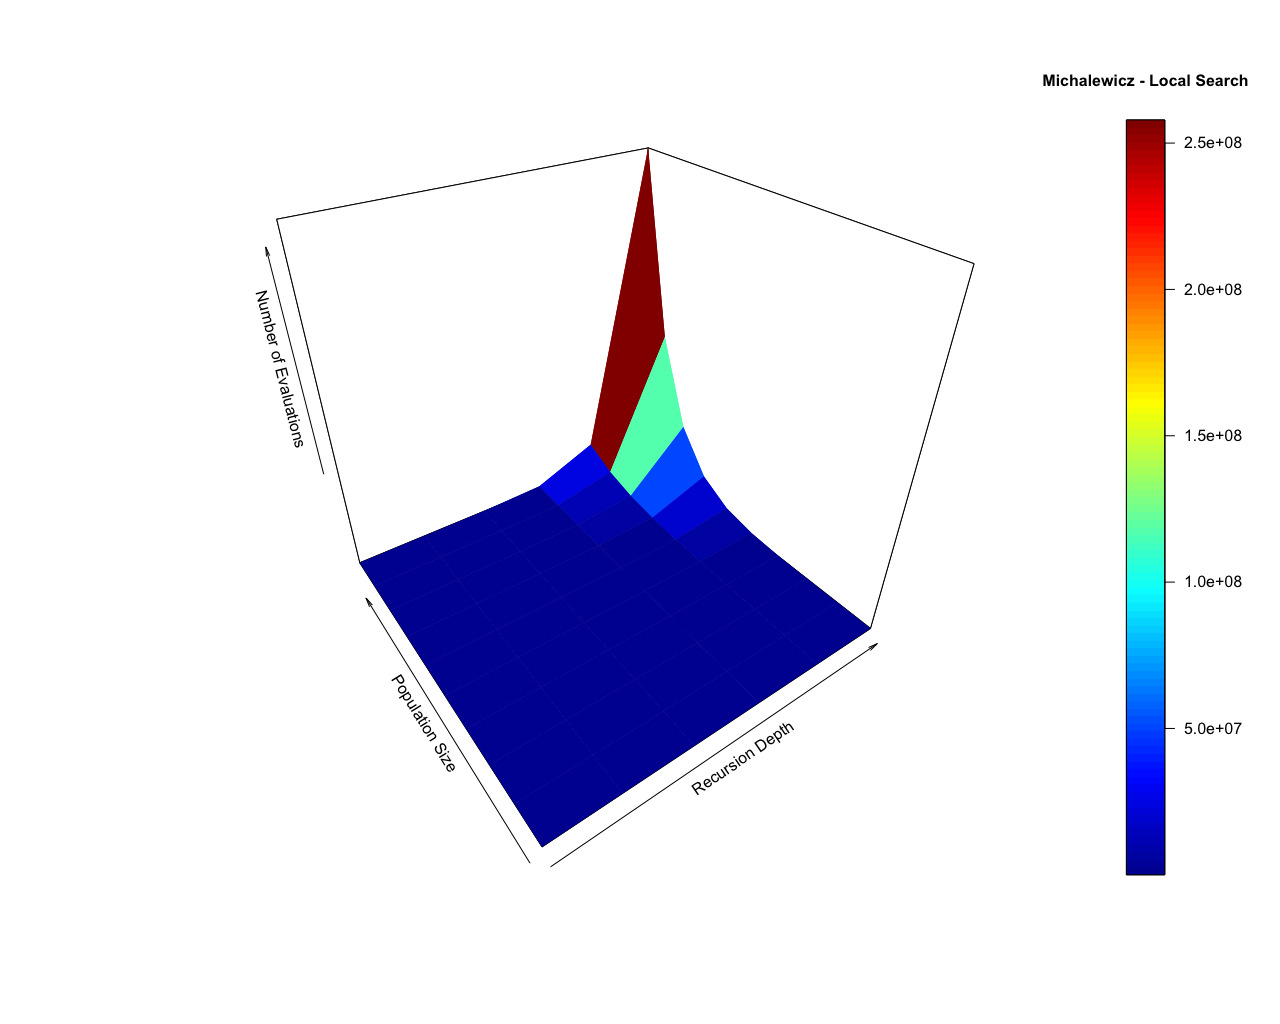
\includegraphics[width=\linewidth]{fig0021.png}
  \subcaption{\tiny Брой смятания на функцията}
  \label{fig0021}
  \end{subfigure}
  \caption{Функцията Michalewicz с локално търсене}
\end{figure}

\begin{figure}[H]
  \begin{subfigure}{0.31\textwidth}
  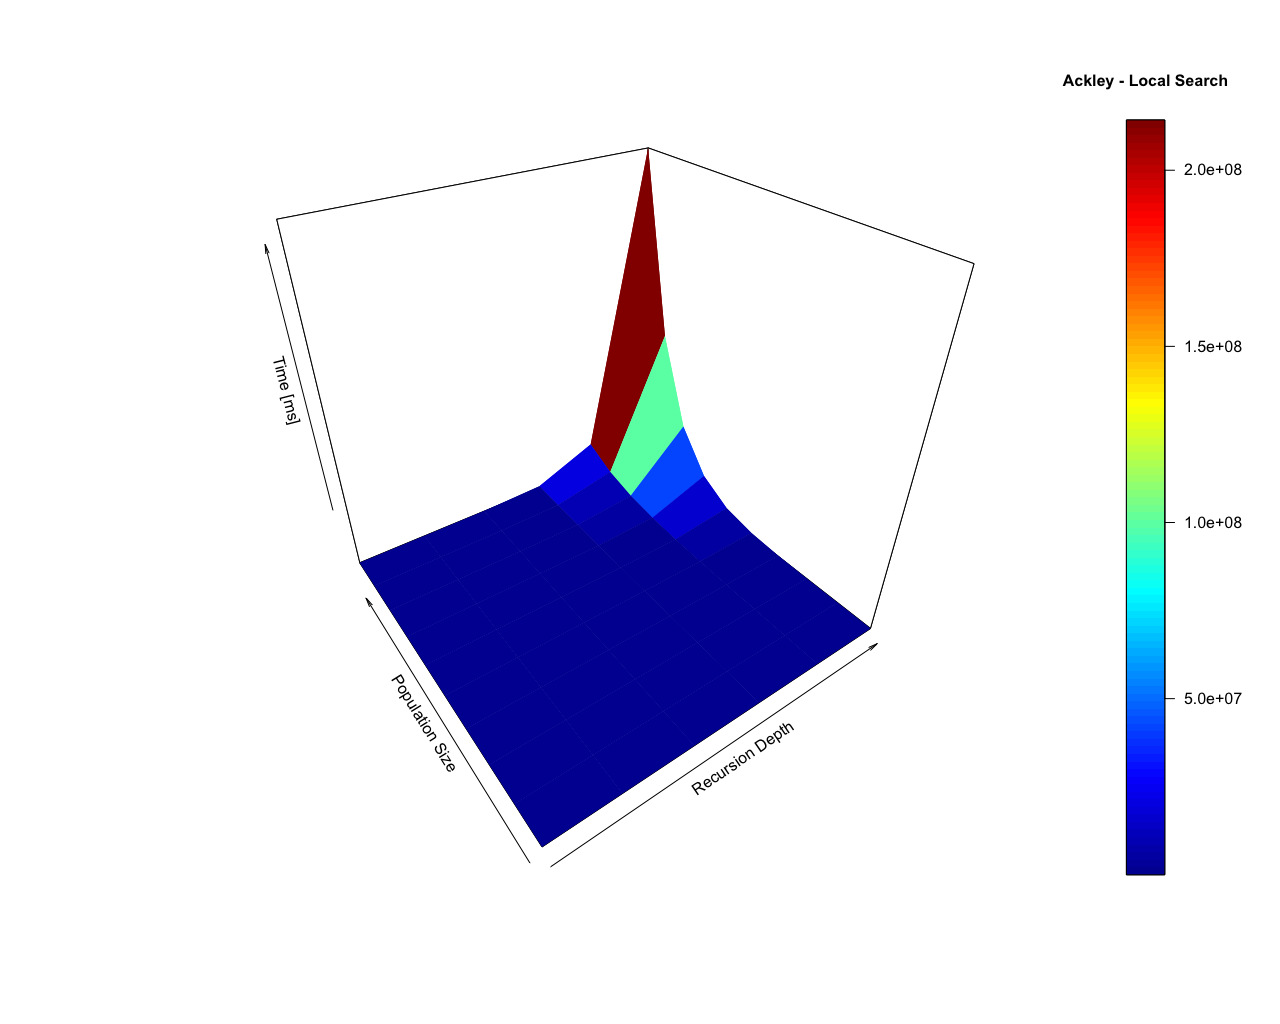
\includegraphics[width=\linewidth]{fig0022.png}
  \subcaption{\tiny Изчислително време [ms]}
  \label{fig0022}
  \end{subfigure}
  \begin{subfigure}{0.31\textwidth}
  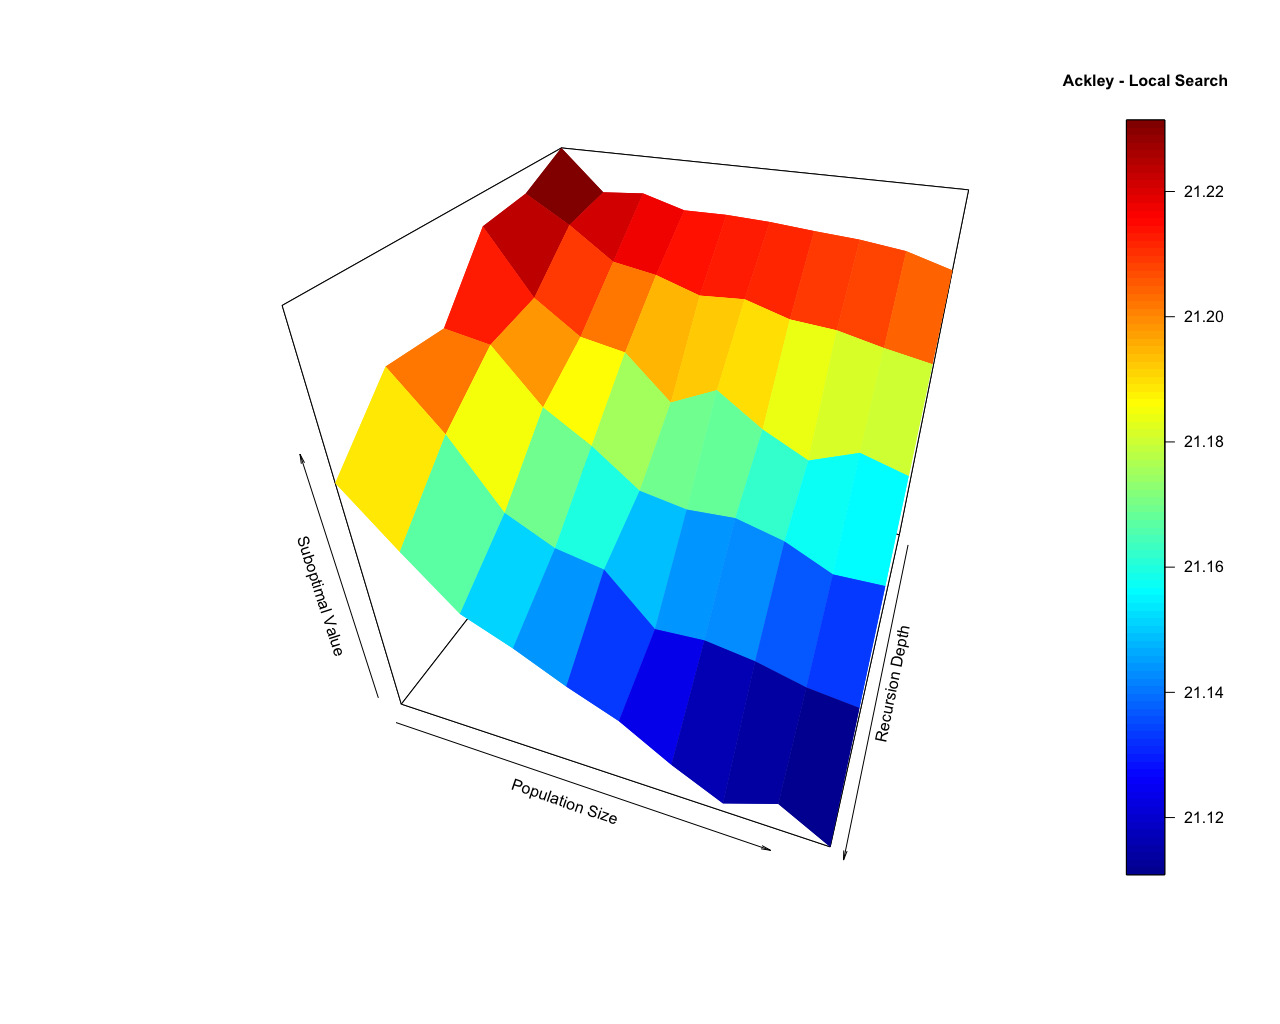
\includegraphics[width=\linewidth]{fig0023.png}
  \subcaption{\tiny Субоптимални стойности}
  \label{fig0023}
  \end{subfigure}
  \begin{subfigure}{0.31\textwidth}
  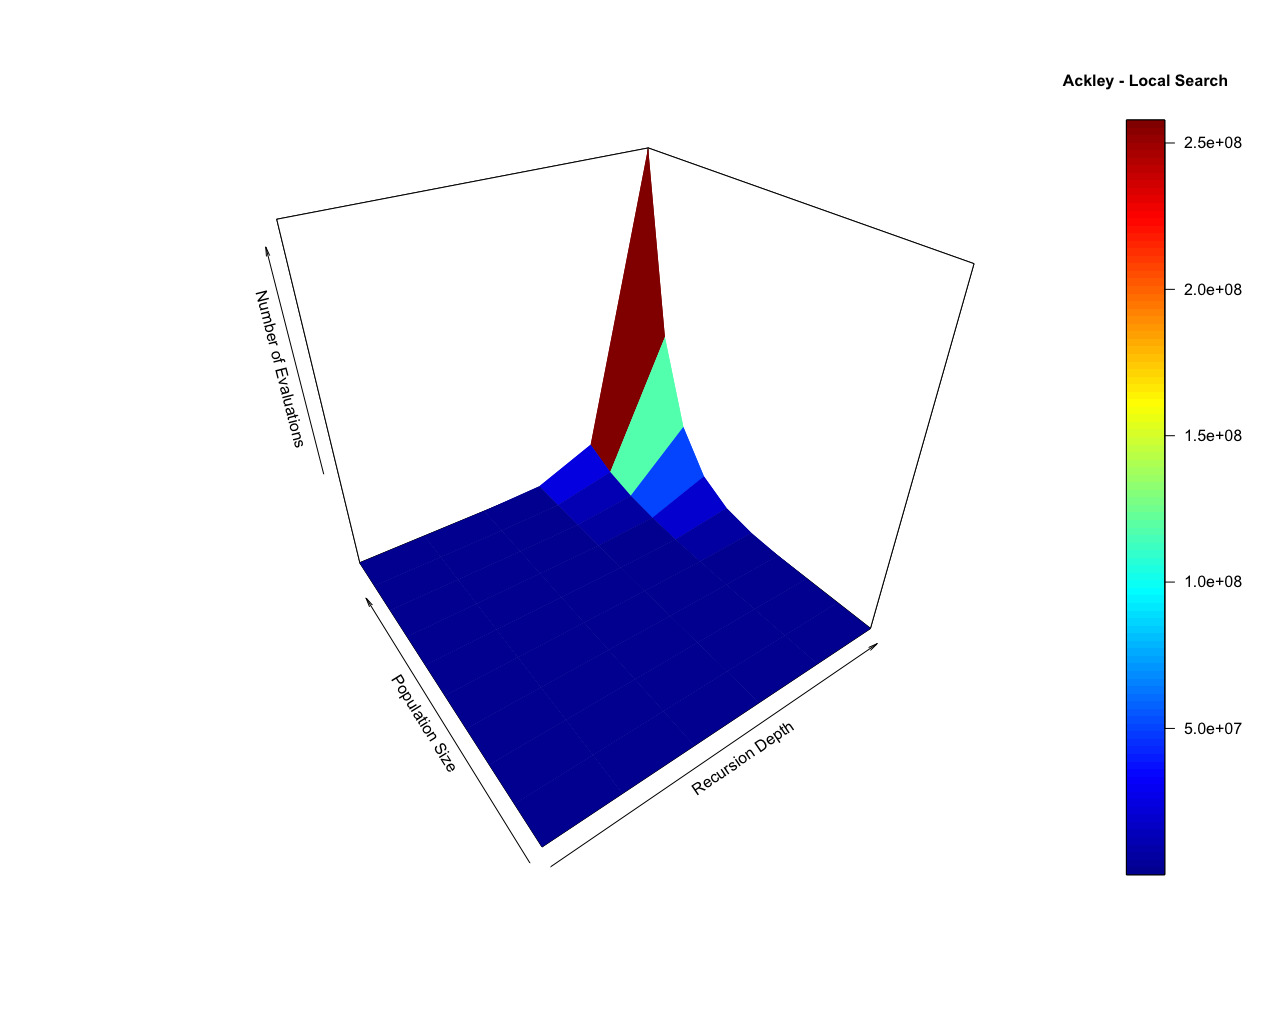
\includegraphics[width=\linewidth]{fig0024.png}
  \subcaption{\tiny Брой смятания на функцията}
  \label{fig0024}
  \end{subfigure}
  \caption{Функцията Ackley с локално търсене}
\end{figure}

\begin{figure}[H]
  \begin{subfigure}{0.31\textwidth}
  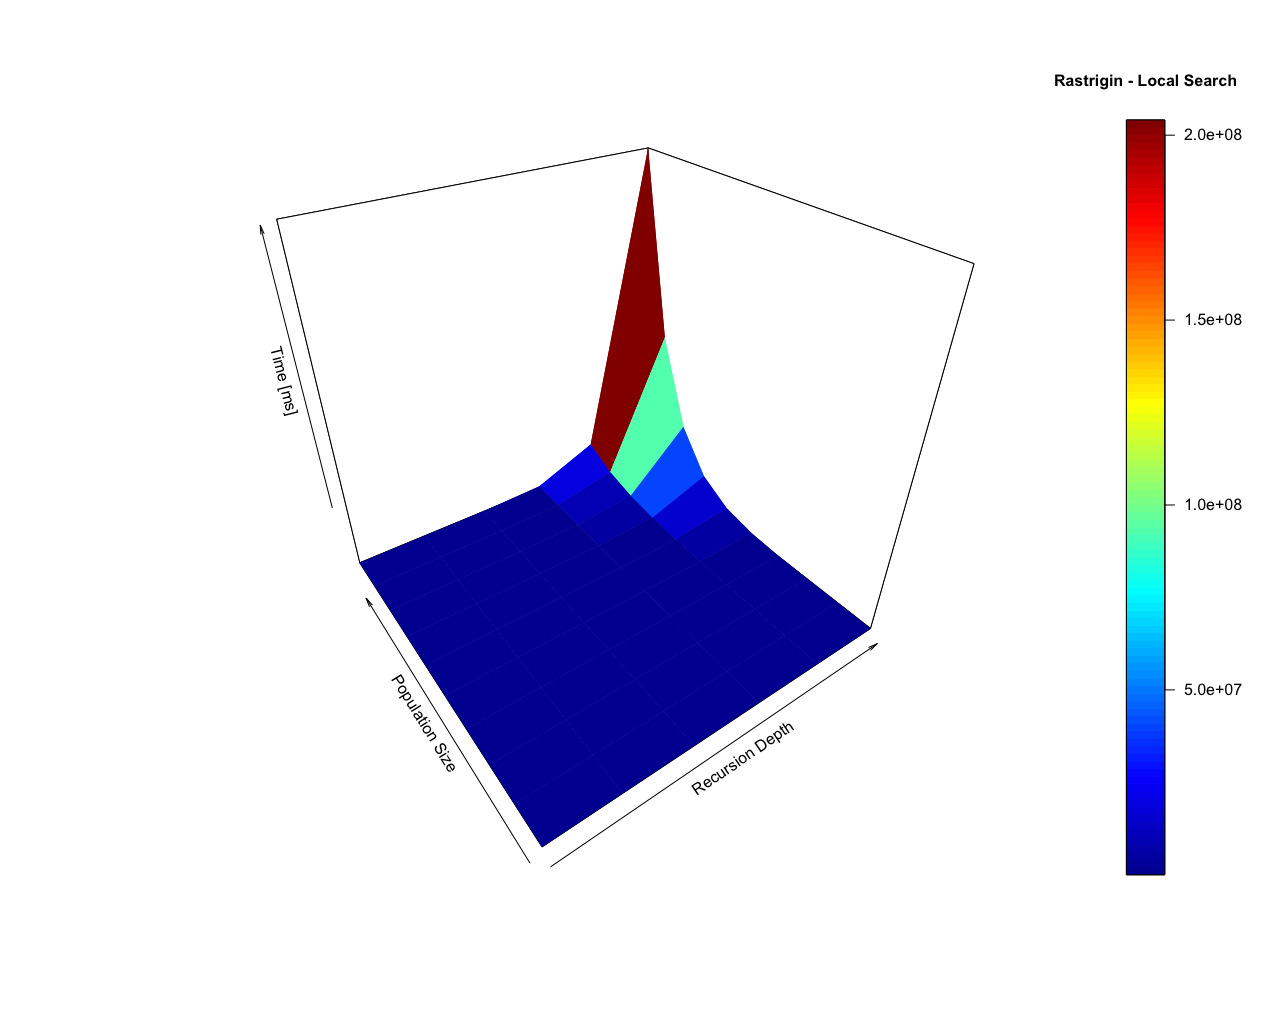
\includegraphics[width=\linewidth]{fig0028.png}
  \subcaption{\tiny Изчислително време [ms]}
  \label{fig0028}
  \end{subfigure}
  \begin{subfigure}{0.31\textwidth}
  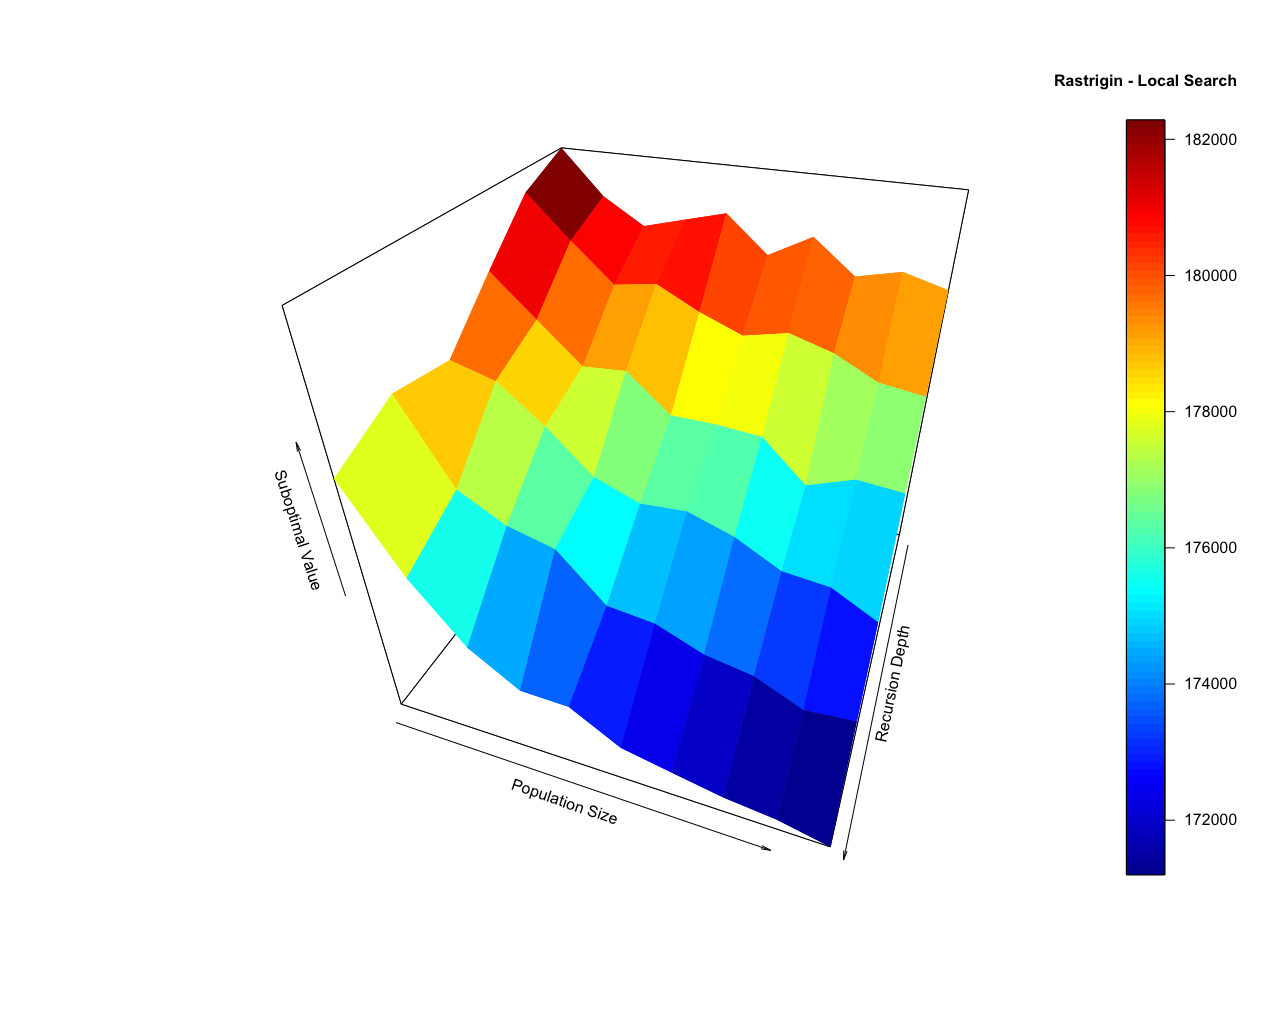
\includegraphics[width=\linewidth]{fig0029.png}
  \subcaption{\tiny Субоптимални стойности}
  \label{fig0029}
  \end{subfigure}
  \begin{subfigure}{0.31\textwidth}
  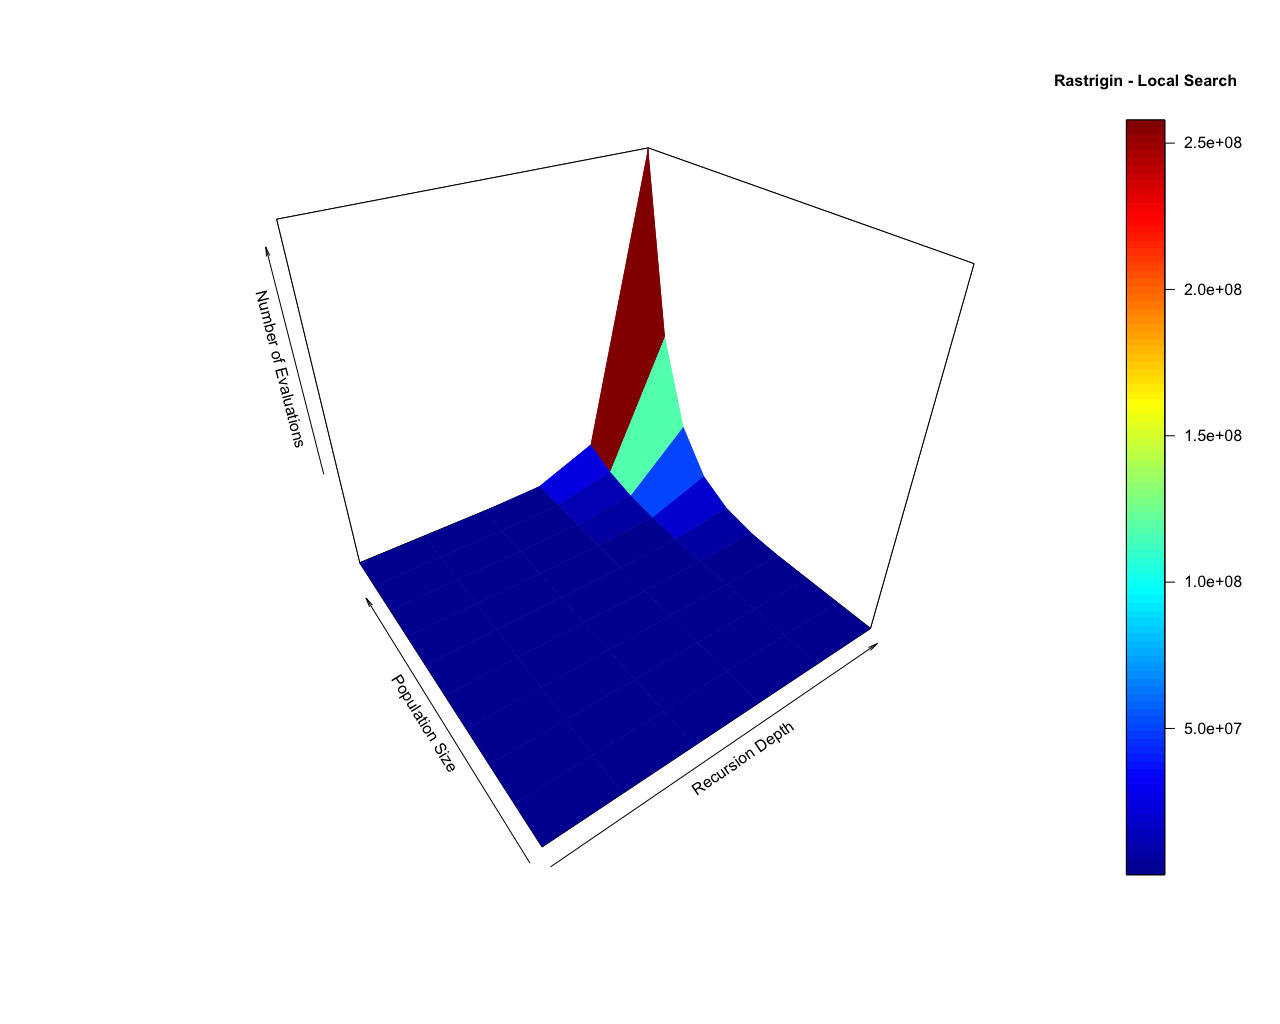
\includegraphics[width=\linewidth]{fig0030.png}
  \subcaption{\tiny Брой смятания на функцията}
  \label{fig0030}
  \end{subfigure}
  \caption{Функцията Rastrigin с локално търсене}
\end{figure}

\begin{figure}[H]
  \begin{subfigure}{0.31\textwidth}
  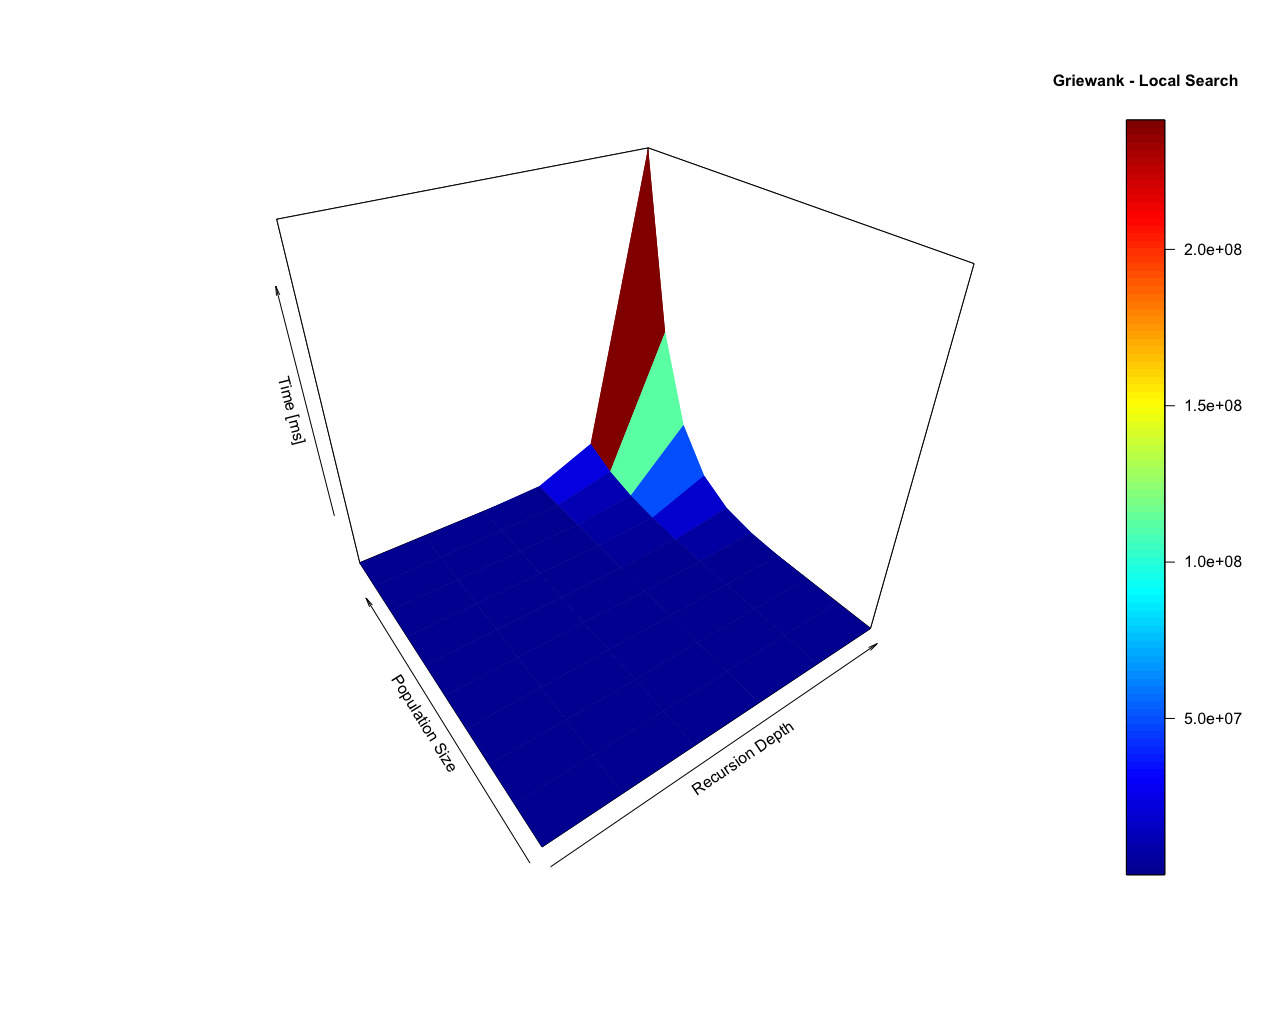
\includegraphics[width=\linewidth]{fig0031.png}
  \subcaption{\tiny Изчислително време [ms]}
  \label{fig0031}
  \end{subfigure}
  \begin{subfigure}{0.31\textwidth}
  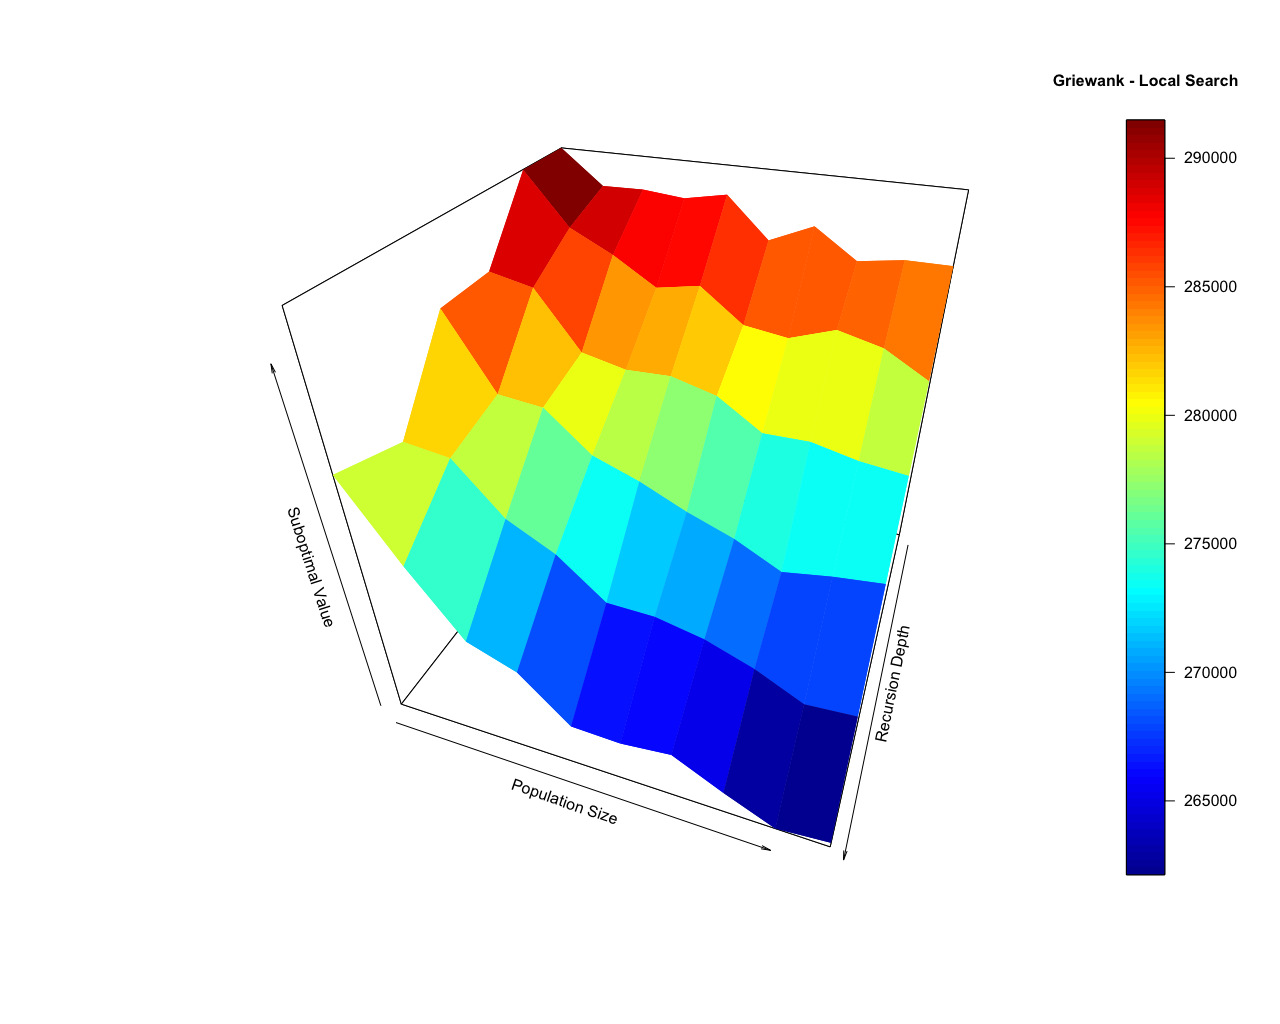
\includegraphics[width=\linewidth]{fig0032.png}
  \subcaption{\tiny Субоптимални стойности}
  \label{fig0032}
  \end{subfigure}
  \begin{subfigure}{0.31\textwidth}
  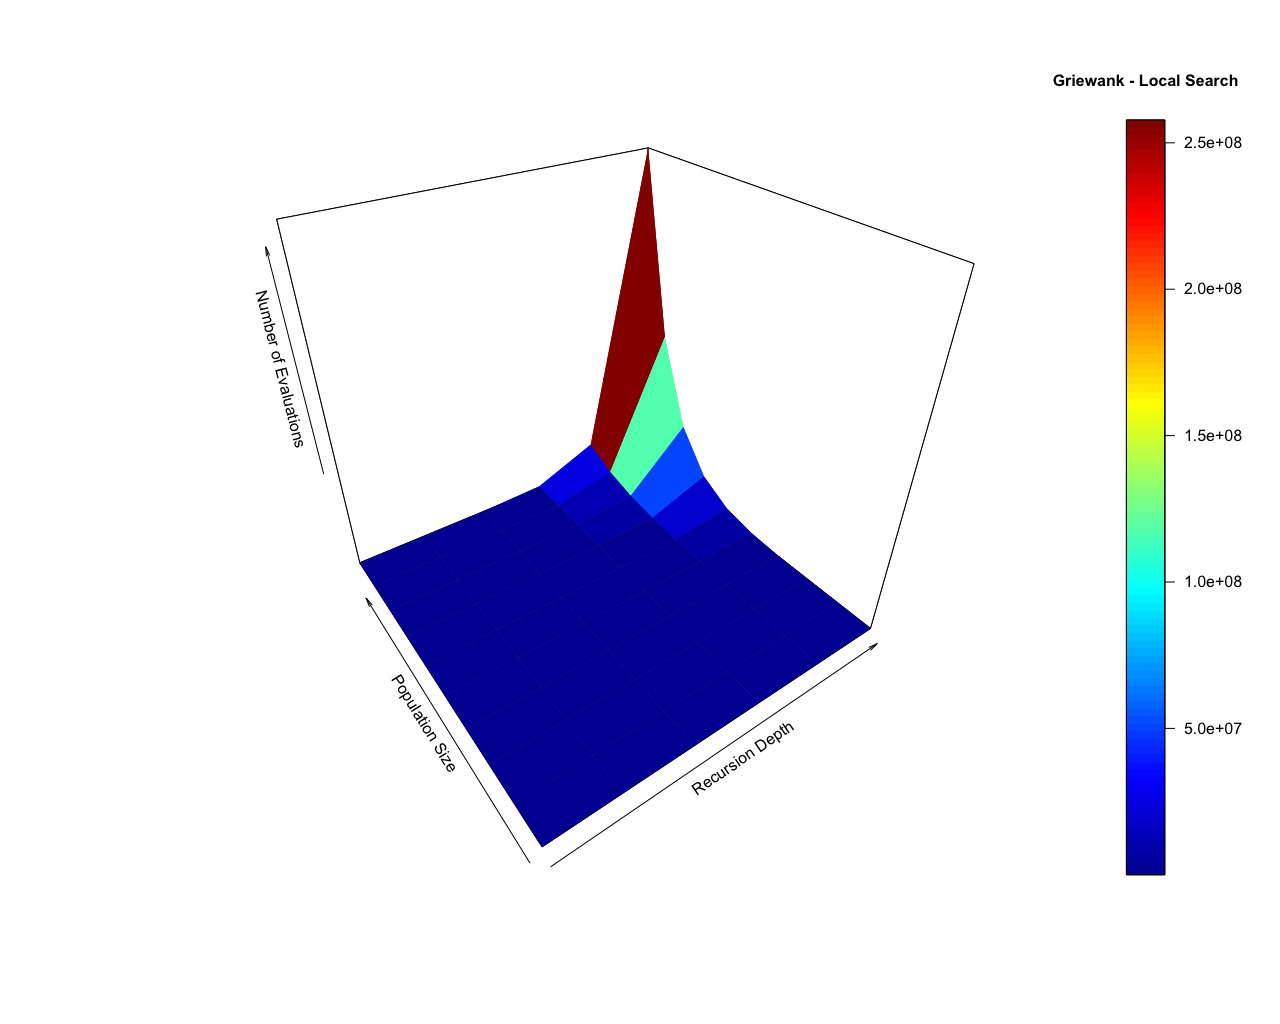
\includegraphics[width=\linewidth]{fig0033.png}
  \subcaption{\tiny Брой смятания на функцията}
  \label{fig0033}
  \end{subfigure}
  \caption{Функцията Griewank с локално търсене}
\end{figure}

\begin{figure}[H]
  \begin{subfigure}{0.31\textwidth}
  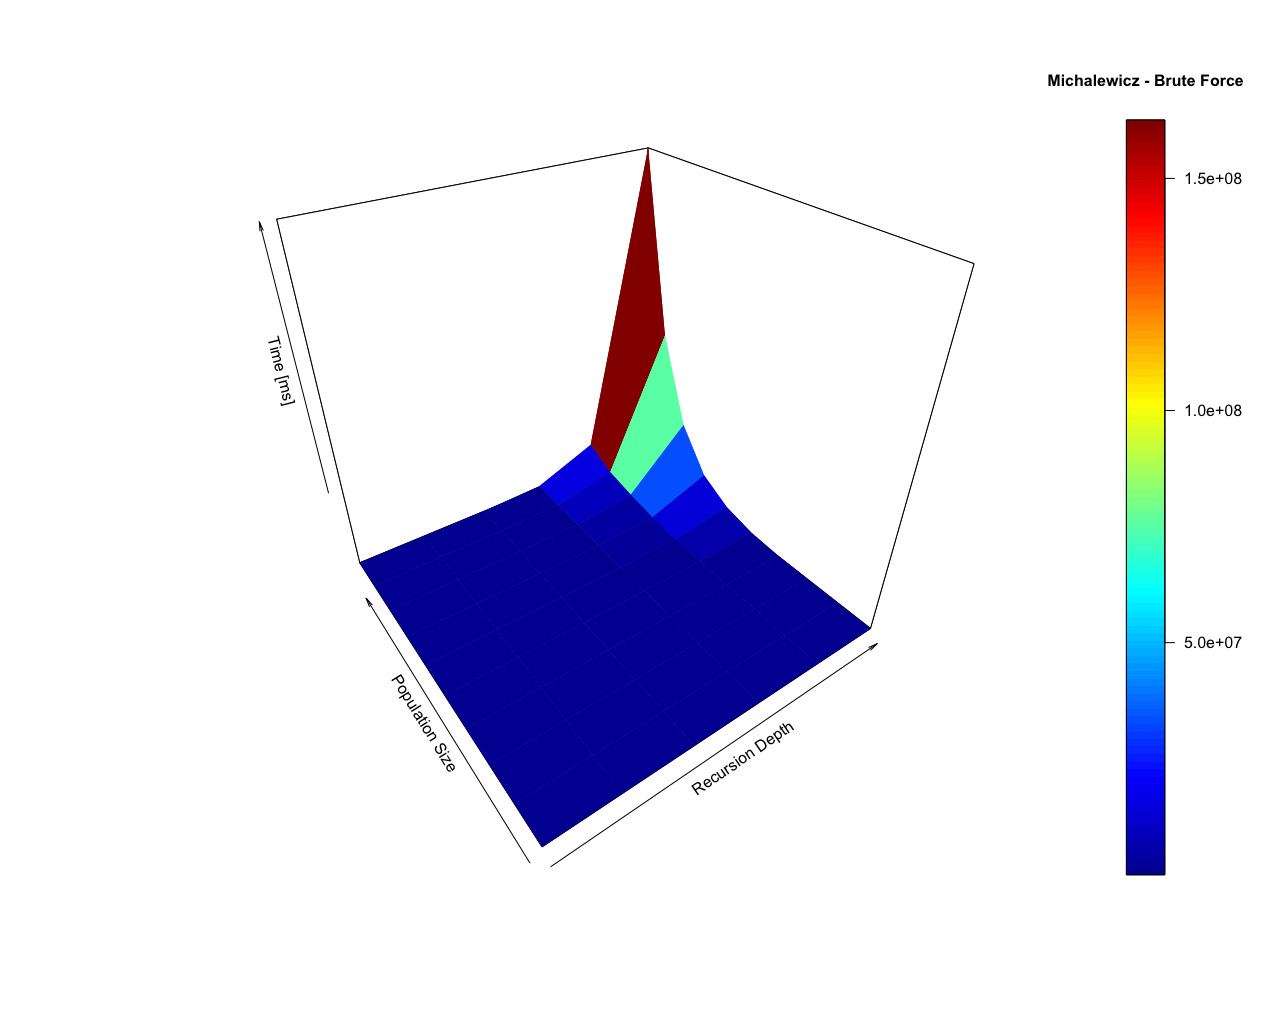
\includegraphics[width=\linewidth]{fig0034.png}
  \subcaption{\tiny Изчислително време [ms]}
  \label{fig0034}
  \end{subfigure}
  \begin{subfigure}{0.31\textwidth}
  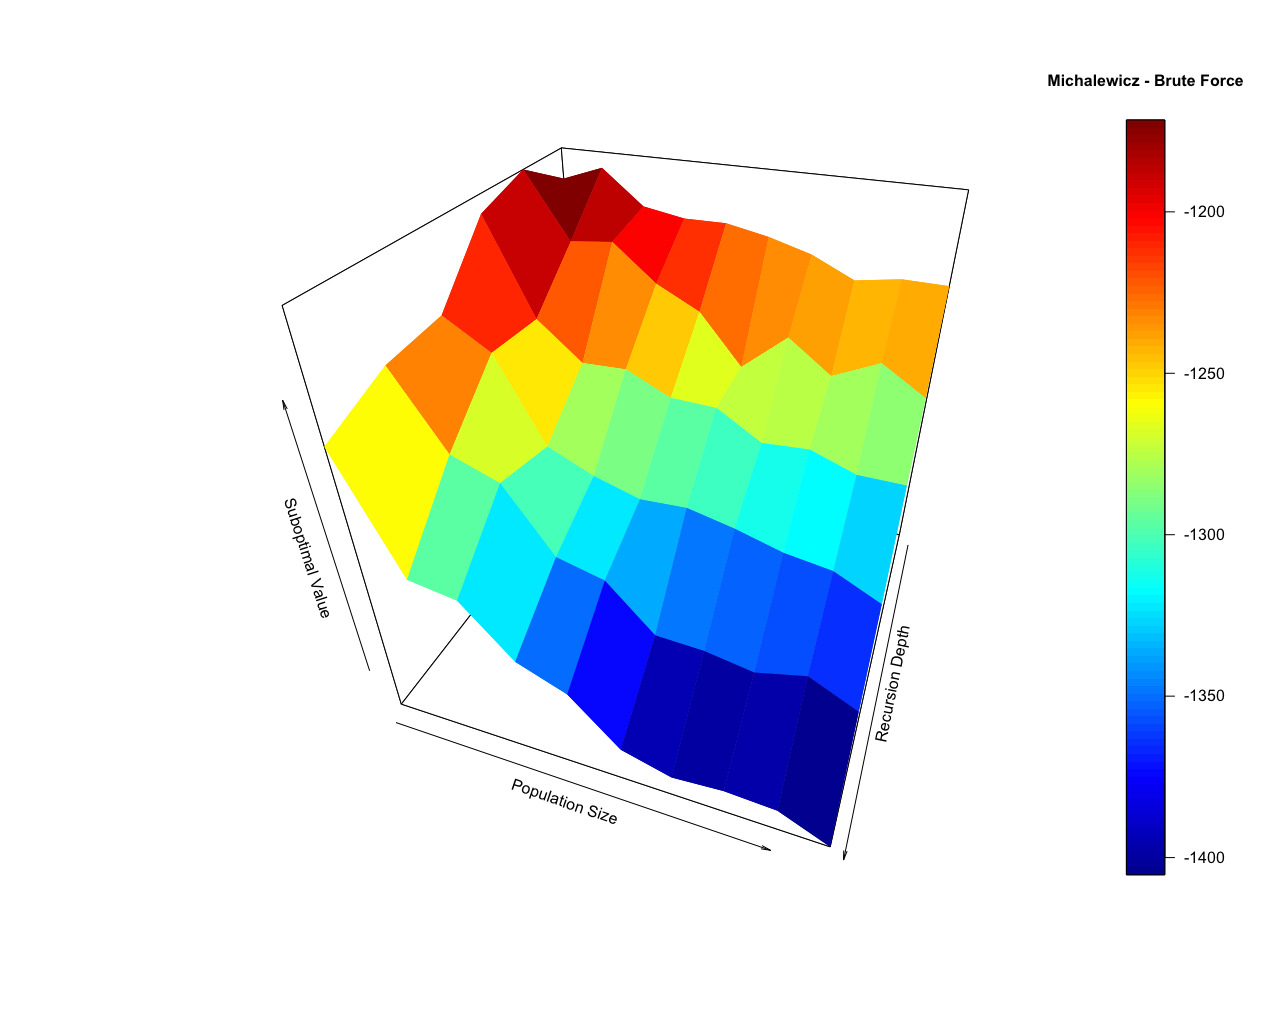
\includegraphics[width=\linewidth]{fig0035.png}
  \subcaption{\tiny Субоптимални стойности}
  \label{fig0035}
  \end{subfigure}
  \begin{subfigure}{0.31\textwidth}
  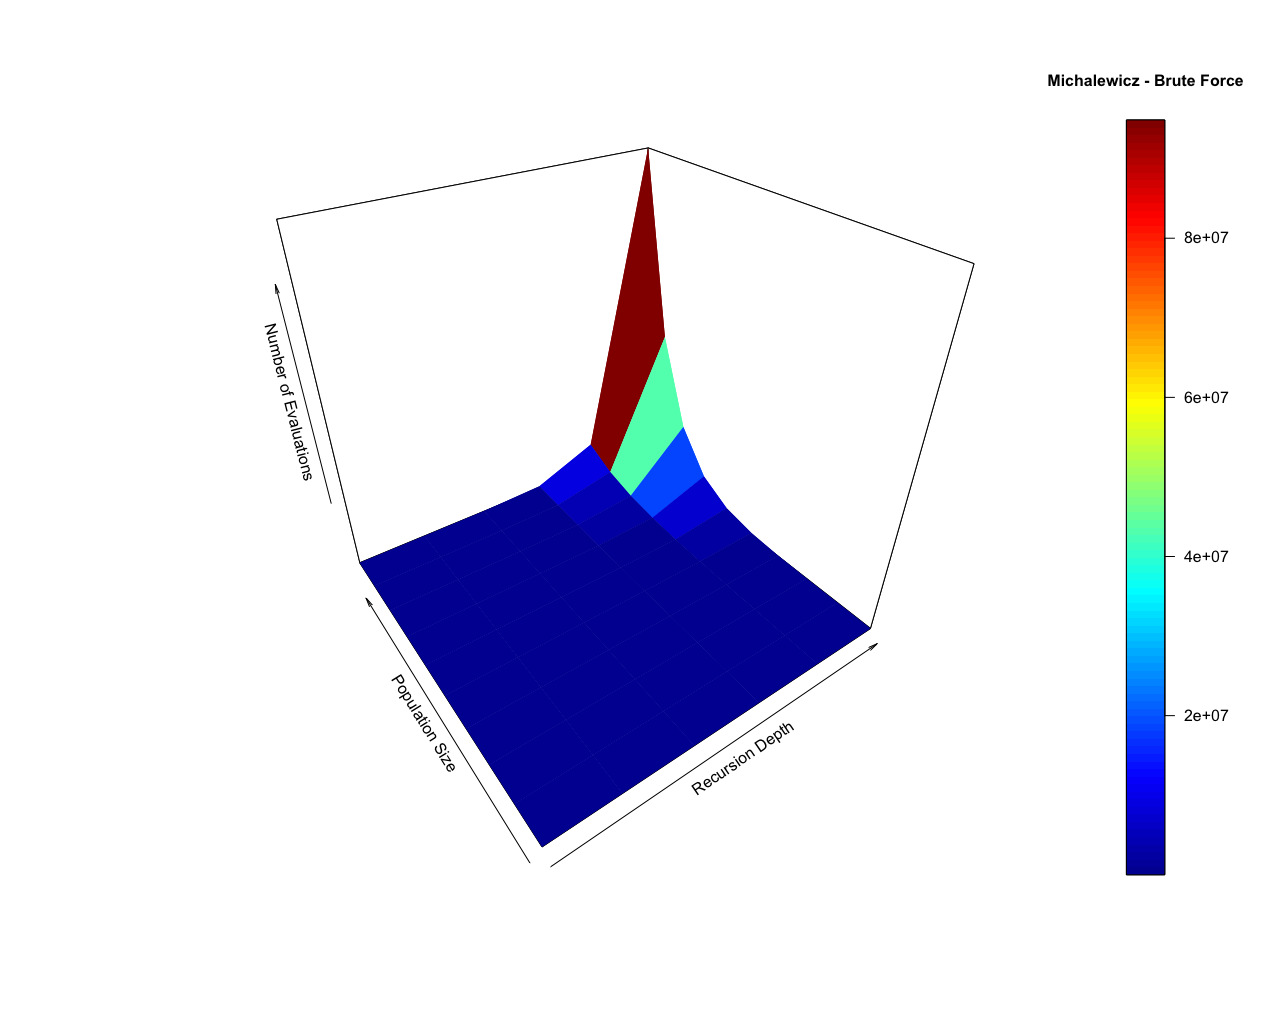
\includegraphics[width=\linewidth]{fig0036.png}
  \subcaption{\tiny Брой смятания на функцията}
  \label{fig0036}
  \end{subfigure}
  \caption{Функцията Michalewicz с пълно изчерпване}
\end{figure}

\begin{figure}[H]
  \begin{subfigure}{0.31\textwidth}
  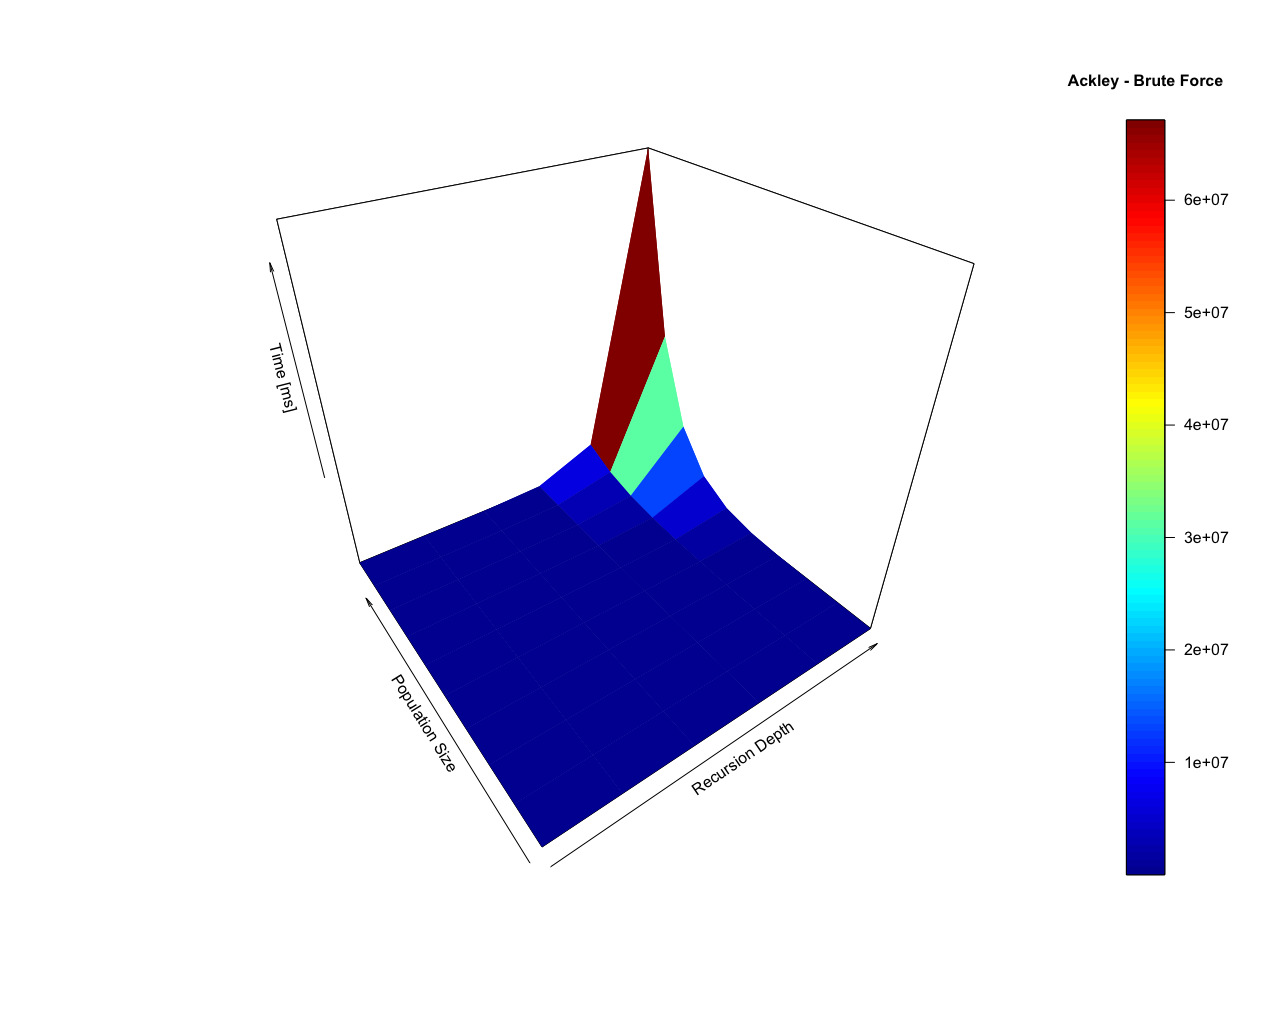
\includegraphics[width=\linewidth]{fig0037.png}
  \subcaption{\tiny Изчислително време [ms]}
  \label{fig0037}
  \end{subfigure}
  \begin{subfigure}{0.31\textwidth}
  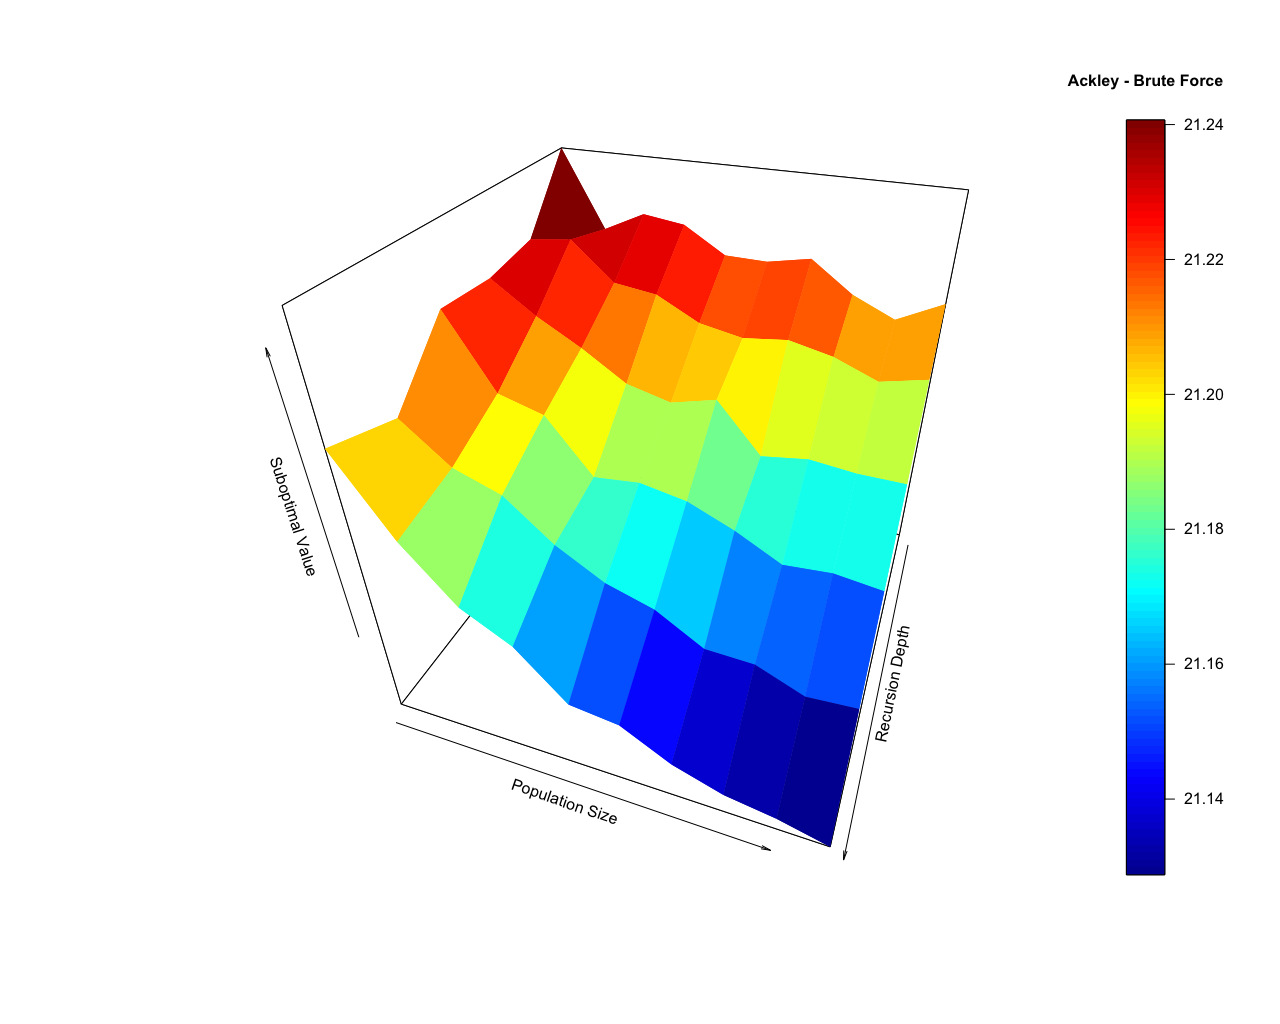
\includegraphics[width=\linewidth]{fig0038.png}
  \subcaption{\tiny Субоптимални стойности}
  \label{fig0038}
  \end{subfigure}
  \begin{subfigure}{0.31\textwidth}
  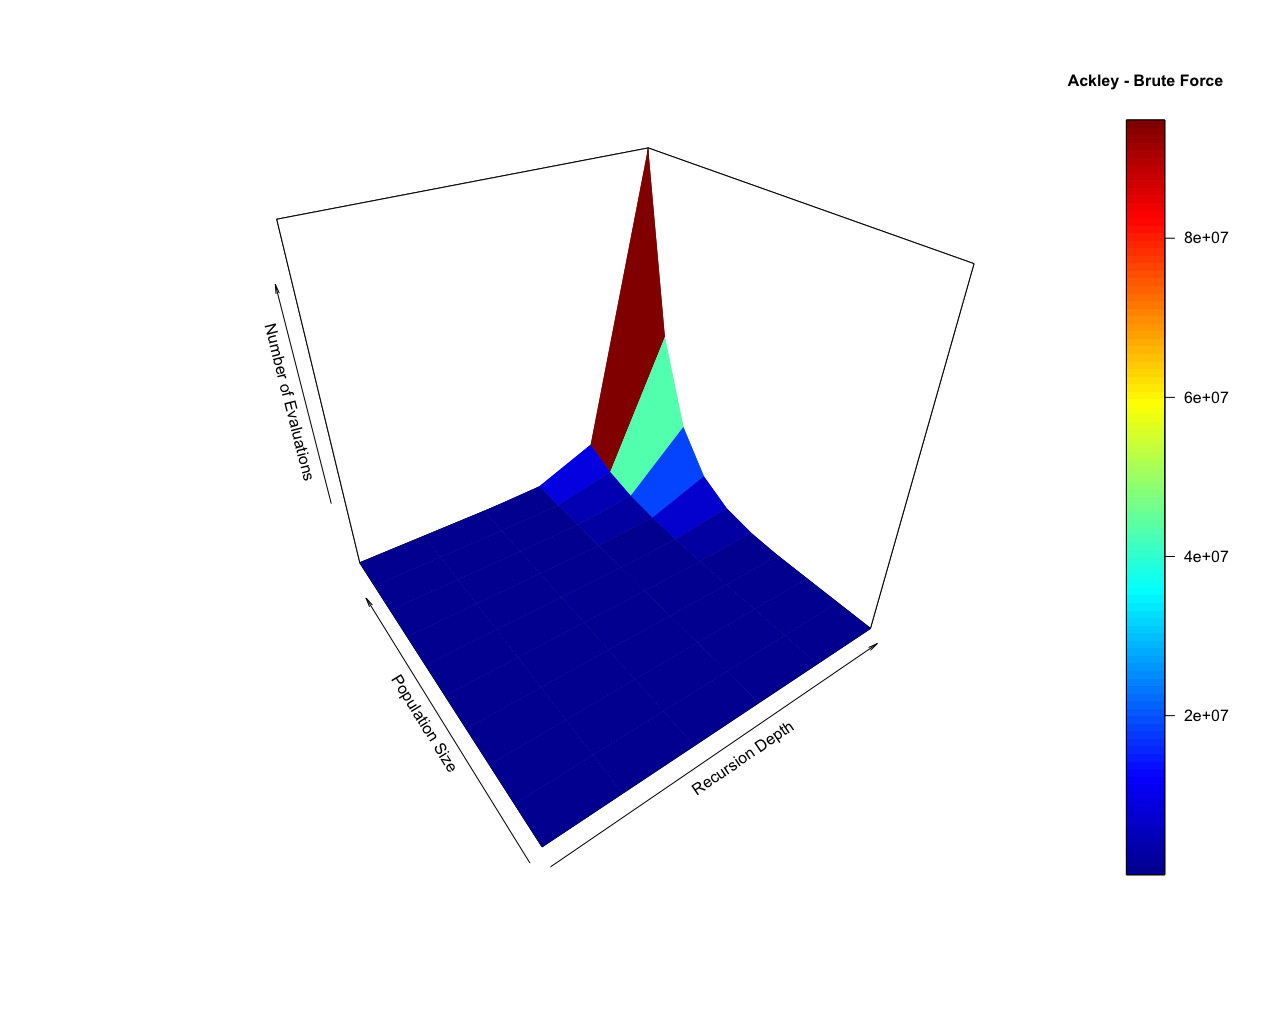
\includegraphics[width=\linewidth]{fig0039.png}
  \subcaption{\tiny Брой смятания на функцията}
  \label{fig0039}
  \end{subfigure}
  \caption{Функцията Ackley с пълно изчерпване}
\end{figure}

\begin{figure}[H]
  \begin{subfigure}{0.31\textwidth}
  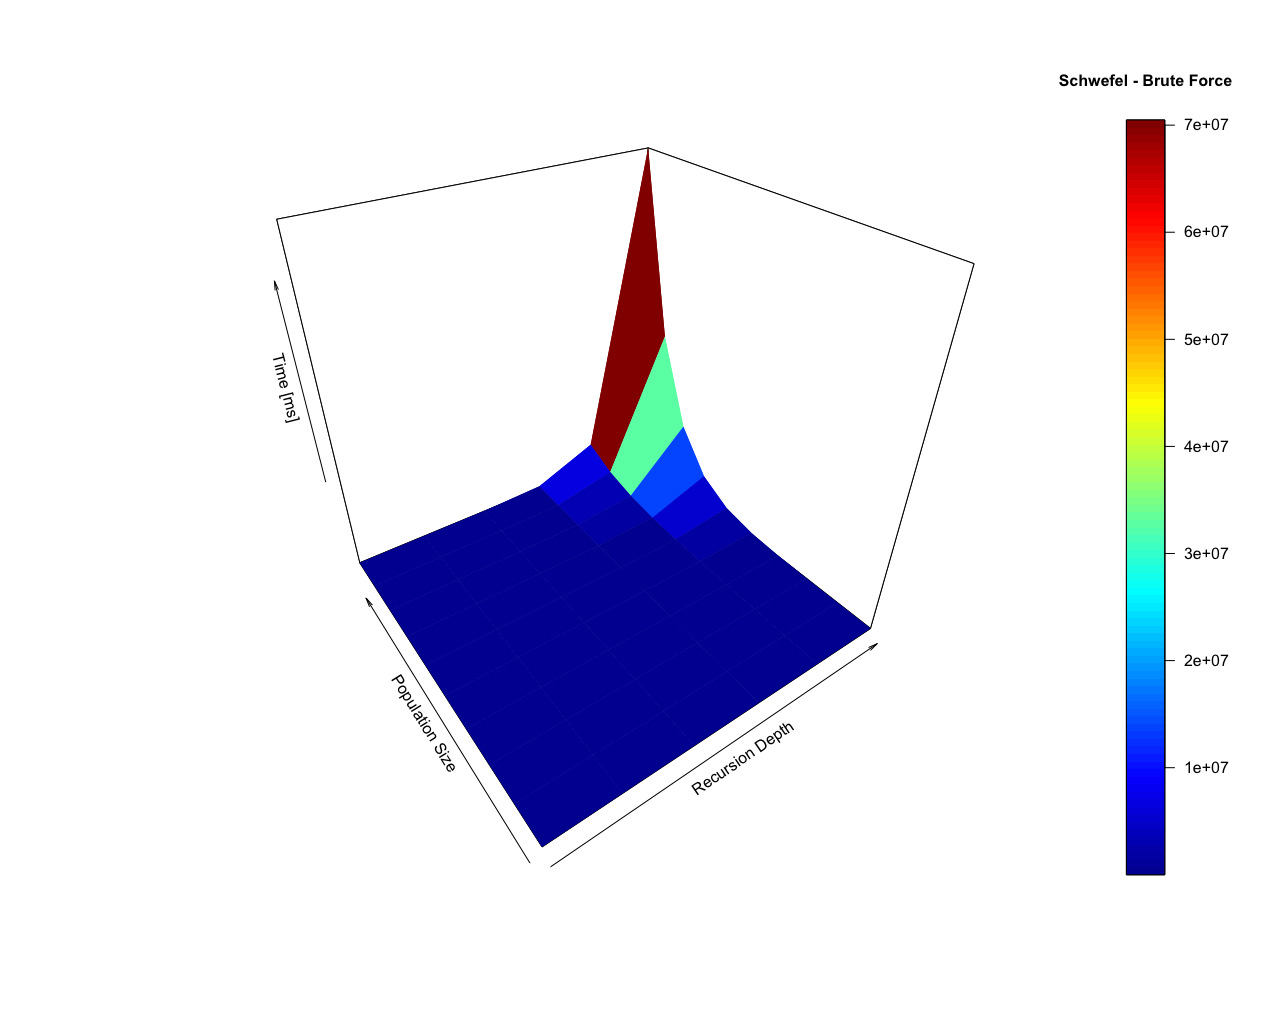
\includegraphics[width=\linewidth]{fig0040.png}
  \subcaption{\tiny Изчислително време [ms]}
  \label{fig0040}
  \end{subfigure}
  \begin{subfigure}{0.31\textwidth}
  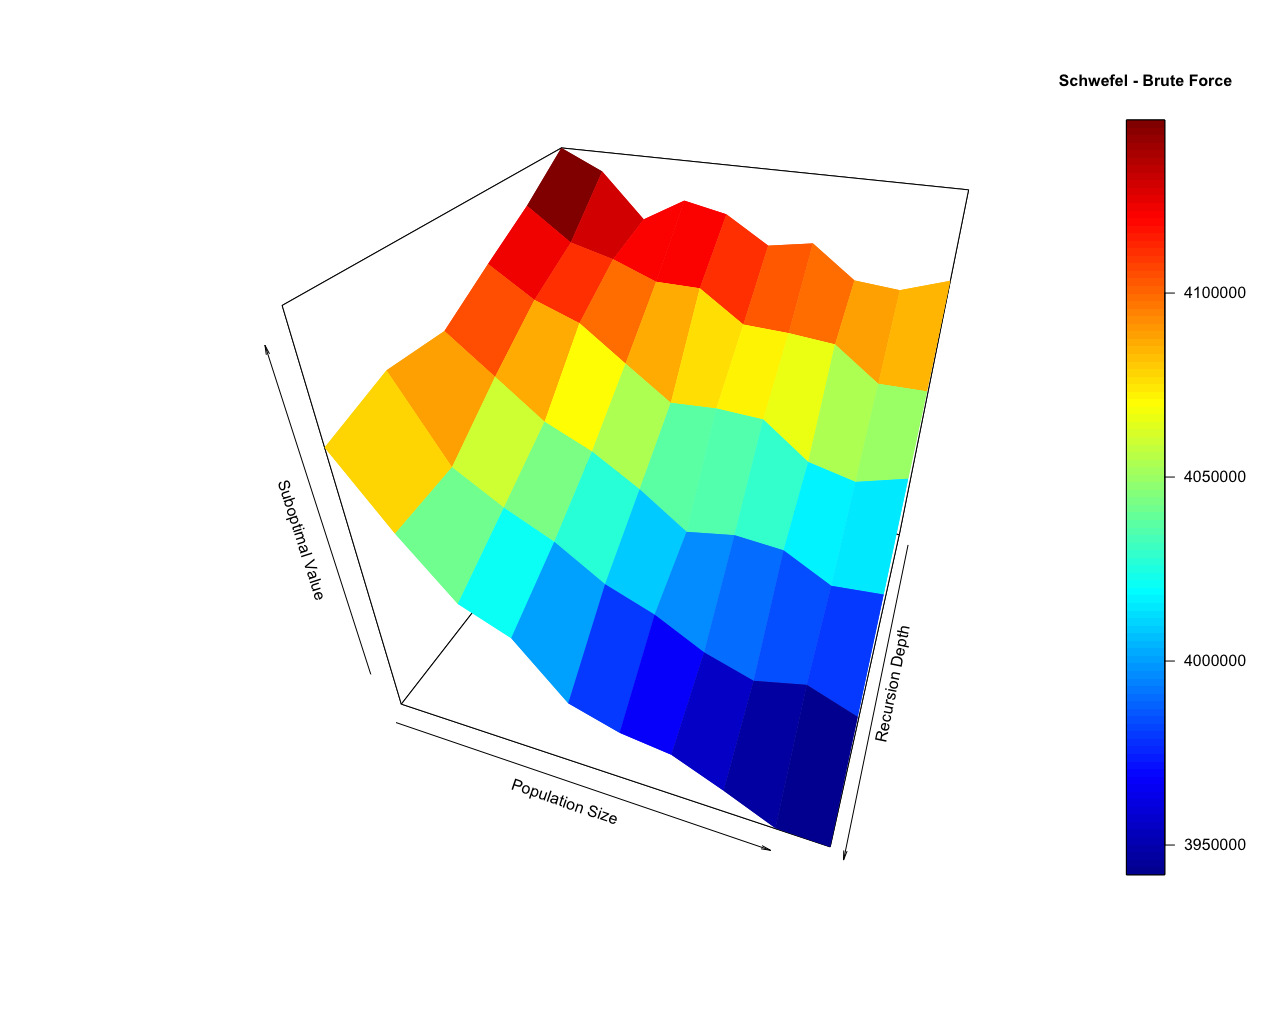
\includegraphics[width=\linewidth]{fig0041.png}
  \subcaption{\tiny Субоптимални стойности}
  \label{fig0041}
  \end{subfigure}
  \begin{subfigure}{0.31\textwidth}
  \includegraphics[width=\linewidth]{fig0042.png}
  \subcaption{\tiny Брой смятания на функцията}
  \label{fig0042}
  \end{subfigure}
  \caption{Функцията Schwefel с пълно изчерпване}
\end{figure}

\begin{figure}[H]
  \begin{subfigure}{0.31\textwidth}
  \includegraphics[width=\linewidth]{fig0043.png}
  \subcaption{\tiny Изчислително време [ms]}
  \label{fig0043}
  \end{subfigure}
  \begin{subfigure}{0.31\textwidth}
  \includegraphics[width=\linewidth]{fig0044.png}
  \subcaption{\tiny Субоптимални стойности}
  \label{fig0044}
  \end{subfigure}
  \begin{subfigure}{0.31\textwidth}
  \includegraphics[width=\linewidth]{fig0045.png}
  \subcaption{\tiny Брой смятания на функцията}
  \label{fig0045}
  \end{subfigure}
  \caption{Функцията Rastrigin с пълно изчерпване}
\end{figure}

\begin{figure}[H]
  \begin{subfigure}{0.31\textwidth}
  \includegraphics[width=\linewidth]{fig0046.png}
  \subcaption{\tiny Изчислително време [ms]}
  \label{fig0046}
  \end{subfigure}
  \begin{subfigure}{0.31\textwidth}
  \includegraphics[width=\linewidth]{fig0047.png}
  \subcaption{\tiny Субоптимални стойности}
  \label{fig0047}
  \end{subfigure}
  \begin{subfigure}{0.31\textwidth}
  \includegraphics[width=\linewidth]{fig0048.png}
  \subcaption{\tiny Брой смятания на функцията}
  \label{fig0048}
  \end{subfigure}
  \caption{Функцията Griewank с пълно изчерпване}
\end{figure}

От извършените експерименти ясно се вижда, че добавката на локално търсене води до по-добри резултати, но това е за сметка на по-дългото време за пресмятане.

\section{Инкрементална апроксимация със синусоиди и тренд}

Тъй като времевите редове представляват измервания, извършени в строга последователност по отношение на оста на времето, получените точки на измерване могат да се подложат на анализ с инструментите за обработка на сигнали. През измерените точки или в близост до тях е възможно да се построят криви (пример е полиномът на Лагранж), описани с математически формули. При достигане на достатъчно близост до точките, надеждата е построените криви да имат поне частични свойства за формиране на прогноза, извън интервала на известните измервания, засягащ бъдещите моменти във времето. В общия случай става въпрос за търсене на подходящи коефициенти в математически формули. Търсенето на подходящите коефициенти е оптимизационна задача със значителна сложност, поради най-често използваните нелинейни компоненти във формулите. Колкото повече коефициенти са обект на оптимизация, толкова по-сложна става оптимизационната задача. По аналогия с трансформацията на Фурие, възможно е през времевия ред да се построи крива изградена от множество синус функции и уравнение на права (обозначава тренда). Теоретично е доказано, че през краен брой точки в двумерното пространство могат да се прекарат безкраен брой криви. Запазването на свойството за обобщение (прогноза) силно зависи от възможността броя синус функции да бъде по-възможност по-малък. 

При финансовите времеви редове е много характерно да има множество флуктуации (движение нагоре или надолу). Тази особеност прави финансовите времеви редове идеални кандидати за апроксимация, чрез ред от синус функции. Във финансовите времеви редове е изключителна рядкост да отсъства тренд. Най-често във финансовите времеви редове се откроява ясно различим тренд на нарастване или тренд на спадане. Трендът ефективно се описва с уравнение на права в двуизмерното пространство, като чрез методи като линейната регресия лесно може да се установят двата параметъра – наклон и срез. 

\begin{equation}  \label{equ001}
y(t) = B.t + C + A_1.sin(\omega_1.t+\varphi_1) + A_2.sin(\omega_2.t+\varphi_2) + ...
\end{equation}

Уравнението за апроксимация чрез тренд и синус функции (\ref{equ001}) съдържа множество коефициенти. Коефициентът $B$ задава наклона на правата. Коефициентът $C$ задава среза в уравнението на правата. Коефициентите $A_n$ задават амплитудата на синус функциите. Коефициентът $\omega_n$ задава ъгловата скорост. Коефициентът $\varphi_n$ задава фазовото отместване. Точният брой синус функции се определя от процедурата по инкрементално оптимизиране на коефициентите. Стремежът е този брой да бъде възможно най-малък, но и изчислените прогнозни стойности да бъдат възможно най-близки до реалните бъдещи стойности. 

\begin{figure}[H]
  \centering
  \includegraphics[width=0.8\linewidth]{fig0007.png}
  \caption{Входни данни за цената на Bitcoin}
\label{fig0007}
\end{figure}

Инкременталният процес по оптимизация започва с оптимизацията само на коефициентите в линейния компонент ($B$ и $C$). Постигнатите оптимални или субоптимални стойности за тренда служат като основа за разширяване на пространството на променливите, като се добавят три коефициента за първата синус функция ($A_1$, $\omega_1$ и $\varphi_1$). Тъй като оптимизаторът използван в LibreOffice Calc е стохастичен, базиран на еволюция на разликите и рояк от частици, процесът по оптимизация се прекратява когато постигнатото най-приближено решение не се подобрява в предварително зададен интервал от време. След изчерпването на възможностите за подобряване на решенията с една синус функция се добавя втора синус функция, която разширява пространството на променливите с още три ($A_2$, $\omega_2$ и $\varphi_2$). Добавянето на синус функции се съблюдава ръчно, тъй като всеки времеви ред се характеризира със своя собствена уникална форма. Важно е да не се добавят твърде много синус функции, защото това би довело до пренапасване на модела (overfitting) и до загуба на възможността за обобщаване (прогнозиране).

\begin{figure}[H]
  \centering
  \includegraphics[width=0.8\linewidth]{fig0008.png}
  \caption{Настройки за оптимизация}
\label{fig0008}
\end{figure}

За демонстрация на описания начин за пресмятане се използват данни за стойността на дигиталната валута Bitcoin в щатски долари, на дневна база, за период от един месец (Фиг. \ref{fig0007}). Стохастичните оптимизационни алгоритми могат да започнат процеса за оптимизация от различни точки в пространството на променливите. Колкото по-благоприятни са началните точки, толкова по-големи са шансовете за достигане на глобално оптимално решение. В предложения пример оптимизацията започва от вектор съдържащ нули във всичките си компоненти. В колона $A$ е зададено времето под формата на числена стойност, според интерпретацията на LibreOffice Calc. В колона $B$ е стойността на отваряне (началото на интервала) за дигиталната валута в съответния ден. В колона $C$ е поместена пресметнатата прогнозна стойност. В колона $D$ е квадратния корен от втората степен на разликата между реалната стойност и прогнозираната стойност. Сумата от всички разлики е пресметната в клетка $M2$ (\ref{fig0008}).

\begin{figure}[H]
  \centering
  \includegraphics[width=0.8\linewidth]{fig0009.png}
  \caption{Коефициенти за уравнение на права}
\label{fig0009}
\end{figure}

След първият цикъл на инкрементална оптимизация оптимизаторът на LibreOffice Calc определя коефициенти за уравнението на правата, която да преминава възможно най-близо до измерените точки (Фиг. \ref{fig0009}). Поради стохастичната природа на двата оптимизатора (еволюция на разликите и рояк от частици), най-често решенията са субоптимални, като доближават глобалния оптимум, но не го достигат гарантирано. Също така, при различни стартирания на цикъла за оптимизация се получават различни субоптимални решения. 

\begin{figure}[H]
  \centering
  \includegraphics[width=0.8\linewidth]{fig0010.png}
  \caption{Включване на първа синус функция}
\label{fig0010}
\end{figure}

След като коефициентите за определяне на тренда бъдат подбрани, следва включване на първа синус функция във втория цикъл от инкременталната оптимизация (Фиг. \ref{fig0010}). Оптимизацията се извършва едновременно за вече определените коефициенти и за ново добавените три коефициента на първата синус функция. Този подход за надграждане дава възможност за допълнителна фина нагласа на коефициентите за тренда. 

\begin{figure}[H]
  \centering
  \includegraphics[width=0.8\linewidth]{fig0011.png}
  \caption{Включване на втора синус функция}
\label{fig0011}
\end{figure}

След като оптимизаторите на LibreOffice Calc достигнат ситуация в която значително подобрение в целевата стойност (клетка $M2$) не се постига (състояние обозначено в решателя като stagnation), следва да се премине към следващ цикъл от инкременталната оптимизация, чрез добавяне на втора синус функция (Фиг. \ref{fig0011}). За конкретните данни от примерния времеви ред, ясно се вижда, че тренд и две синус функции водят до добро напасване и имат нужните свойства за изчисляване на прогнозни стойности. При времеви редове с повече на брой измервания и повече на брой флуктуации, броят на синус функциите би бил по-голям. 

\begin{figure}[H]
  \centering
  \includegraphics[width=0.8\linewidth]{fig0012.png}
  \caption{Включване на трета синус функция}
\label{fig0012}
\end{figure}

За да се подбере точния момент в който трябва да се преустанови добавянето на синус функции се съблюдават разликите в целевата клетка на оптимизацията (клетка $M2$). При добавянето на трета синус функция (Фиг. \ref{fig0012}) се забелязва, че целевата клетка не променя драстично стойността си. Изборът до коя на брой синус функция да се прекрати инкременталната оптимизация остава изцяло субективен и от компетентността на лицето вземащо решения на база на генерираните прогнози. 

\section{Бърз прототип на LibreOffice Calc с еволюция на разликите и оптимизация с рояк от частици}

Процесът по търсенето на оптимални тегла в изкуствена невронна мрежа от тип трислоен перцептрон много нагледно може да бъде демонстриран с бърз прототип в софтуерния пакет LibreOffice Calc. За осъществяване на прототипирането моделът на изкуствената невронна мрежа бива разгърнат в двузимерната равнина от клетки на електронната таблица. Търсенето на оптимални стойности за теглата в мрежата се постига чрез вградения в LibreOffice Calc модул за оптимизация наречен Solver (Фиг. \ref{fig0001}).

\begin{figure}[H]
  \centering
  \includegraphics[width=0.8\linewidth]{fig0001.png}
  \caption{Модул за оптимизация в LibreOffice Calc}
\label{fig0001}
\end{figure}

За нелинейна оптимизация модулът прилага алгоритмите за еволюция на разликите и оптимизация с рояк от частици. Двата алгоритъма се прилагат в хибридна комбинация, като с предварително дефинирана вероятност е определено колко често ще бъде активиран всеки от тях. Модулът се настройва за клетка, чиято оптимална стойност ще бъде търсена (максимум, минимум или конкретно число). Също така, задава се и регионът от клетки, които подлежат на промяна в процеса по оптимизация. Като клетка в която ще се търси минимум при бързото протитипиране се избира общата средно-квадратична грешка допусната от изкуствената невронна мрежа. Регионът от клетки за оптимизация съдържа теглата използевани в изкуствената невронна мрежа. 

\begin{figure}[H]
  \centering
  \includegraphics[width=0.8\linewidth]{fig0002.png}
  \caption{Стойности на Bitcoin виртуалната валута}
\label{fig0002}
\end{figure}

Като множество данни се използват стойностите на Bitcoin виртуалната валута (Фиг. \ref{fig0002}), на дневна база, за няколко години назад. Моделът за прогнозиране се основава на нелинейна авторегресия. Това означава, че на входа на мрежата се подават мащабирани минали стойности от времевия ред, а на изхода на мрежата се очакват мащабирани прогнозни стойности. 

\begin{figure}[H]
  \centering
  \includegraphics[width=0.8\linewidth]{fig0003.png}
  \caption{Параметри на трислойната изкуствена невронна мрежа}
\label{fig0003}
\end{figure}

След подбора на времеви ред следва избор на параметрите с които ще бъде напревен модела на трислойната изкуствена невронна мрежа (Фиг. \ref{fig0003}). За целите на линейното мащабиране първо се намират най-малката и най-голямата стойност в оригиналния времеви ред, чрез формули в LibreOffice Calc: $=MIN(A:A)$ и $=MAX(A:A)$. Тъй като приложената прагова функция е хиперболичен тангенс, диапазона за мащабирания времеви ред е избран от -0.5 до +0.5. Умишлено се избягва мащабиране до асимптотичните стойности от -1.0 до +1.0, тъй като такова мащабиране много би увеличило стойностите на междинните пресмятания, а и не би дало възможност да се прогнозират по-малки или по-големи стойности от вече известните в оригиналния времеви ред. Топологията на мрежата се избира експериментално, като изходния слой има размер, според това колко стойности в бъдещето е желателно да се предсказват. Размера на входния слой се определя експериментално. За размера на скрития слой има различни емпирични правила, като най-популярното е скритият слой да бъде половината от сумата на размерите имащи входния и изходния слой. Съществуват адаптивни алгоритми, които чрез проби и грешки да определят топологията на мрежата, но в това бързо прототипиране тези алгоритми не се прилагат. 

Общият брой стойности в оригиналния времеви ред се определят с формула в LibreOffice Calc: $=COUNT(A:A)$. Тъй като процеса по „разгръщането“ на модела е относително бавен, то се добавя клетка в която да се проследява напредъка от Python скрипта в „разгръщането“. LibreOffice Calc позволява изпълнението на макроси, като се поддържат няколко програмни езика. Програмният език Python е изключително популярен в сферата на машинното самообучение и дава изключително големи възможности за частична автоматизация в програмите на LibreOffice.

След мащабирането на оригиналния времеви ред се формират тренировъчните примери, като за вход се вземат стойности преди условния момент $t_0$, а за очакван изход стойности след условния момент $t_0$ (условно разделяне на минало и бъдеще).

\begin{lstlisting}[caption=Мащабиране на оригиналния времеви ред, language=Python, basicstyle=\tiny, label=list0001]
    ''' Scale input. '''
    for t in range(1, total_values + 1):
        sheet.getCellRangeByName("E" + str(t)).setValue(sheet.getCellRangeByName("$C$4").getValue() + 
        (sheet.getCellRangeByName("$C$5").getValue() - sheet.getCellRangeByName("$C$4").getValue()) * ((sheet.getCellRangeByName("A" + str(t)).getValue() - 
        sheet.getCellRangeByName("$C$1").getValue()) / (sheet.getCellRangeByName("$C$2").getValue() - sheet.getCellRangeByName("$C$1").getValue())))
\end{lstlisting}

В листинг \ref{list0001} се демонстрира линейното мащабиране, като за извършване на изчисленията се използват установените минимални и максимални стойности (Фиг. \ref{fig0004}). 

\begin{figure}[H]
  \centering
  \includegraphics[width=0.8\linewidth]{fig0004.png}
  \caption{Резултат от мащабирането на времевия ред}
\label{fig0004}
\end{figure}

На всеки слой в изкуствената невронна мрежа се добавя по един допълнителен неврон (Листинг \ref{list0002}), постоянно емитиращ единична стойност (отместване или от английски език bias).

\begin{lstlisting}[caption=Неврони емитиращи постоянно единичен сигнал, language=Python, basicstyle=\tiny, label=list0002]
        ''' Setup biases. '''
        sheet.getCellRangeByName("G" + str(x)).setValue(1)
        sheet.getCellRangeByName("G" + str(x)).CellBackColor = (255 << 16 | 255 << 8 | 0)
        sheet.getCellRangeByName("H" + str(x)).setValue(1)
        sheet.getCellRangeByName("H" + str(x)).CellBackColor = (255 << 16 | 255 << 8 | 0)
        sheet.getCellRangeByName("I" + str(x)).setValue(1)
        sheet.getCellRangeByName("I" + str(x)).CellBackColor = (255 << 16 | 255 << 8 | 0)
        sheet.getCellRangeByName("J" + str(x)).setValue(1)
        sheet.getCellRangeByName("J" + str(x)).CellBackColor = (255 << 16 | 255 << 8 | 0)
\end{lstlisting}

Мащабираният времеви ред бива „разбит“ условно на „минали“ стойности и „бъдещи“ стойности. Миналите стойности стават входни сигнали за изкуствената невронна мрежа (Листинг \ref{list0003}).

\begin{lstlisting}[caption=Формиране на входния слой, language=Python, basicstyle=\tiny, label=list0003]
        ''' Input data loading. '''
        for i in range(1, input_size + 1):
            sheet.getCellRangeByName("G" + str(x + i)).setValue(sheet.getCellRangeByName("E" + str(t + i)).getValue())
            sheet.getCellRangeByName("G" + str(x + i)).CellBackColor = (255 << 16 | 0 << 8 | 0)
\end{lstlisting}

По аналогичен начин, будещите стойности се зареждат като очакван изход от изкуствената невронна мрежа (Листинг \ref{list0004}).

\begin{lstlisting}[caption=Очакван изход от мрежата, language=Python, basicstyle=\tiny, label=list0004]
        ''' Expected data loading. '''
        for e in range(1, output_size + 1):
            sheet.getCellRangeByName("J" + str(x + e)).setValue(sheet.getCellRangeByName("E" + str(t + e + input_size)).getValue())
            sheet.getCellRangeByName("J" + str(x + e)).CellBackColor = (0 << 16 | 127 << 8 | 0)
\end{lstlisting}

Стойностите във възлите на скрития слой са резултат от пресмятане на входните сигнали и текущите стойности на теглата в мрежата (Листинг \ref{list0005}). 

\begin{lstlisting}[caption=Стойности на скрития слой при правия пас, language=Python, basicstyle=\tiny, label=list0005]
        ''' Setup hidden layer. '''
        wih = 1
        for h in range(1, hidden_size + 1):
            sum = ""
            for i in range(0, input_size + 1):
                sum = sum + "G" + str(x + i) + "*Q" + str(wih)
                wih = wih + 1
                if i < input_size:
                    sum = sum + " + "
            sheet.getCellRangeByName("H" + str(x + h)).setFormula("=TANH( " + sum + " )")
            sheet.getCellRangeByName("H" + str(x + h)).CellBackColor = (0 << 16 | 0 << 8 | 255)
\end{lstlisting}

На свой ред, стойностите в изходния слой са резултат от пресмятане на сигналите в скрития слой и текущите стойности на теглата в мрежата (Листинг \ref{list0006}).

\begin{lstlisting}[caption=Стойности на изходния слой при правия пас, language=Python, basicstyle=\tiny, label=list0006]
        ''' Setup output layer. '''
        who = 1
        for o in range(1, output_size + 1):
            sum = ""
            for h in range(0, hidden_size + 1):
                sum = sum + "H" + str(x + h) + "*S" + str(who)
                who = who + 1
                if h < hidden_size:
                    sum = sum + " + "
            sheet.getCellRangeByName("I" + str(x + o)).setFormula("=TANH( " + sum + " )")
            sheet.getCellRangeByName("I" + str(x + o)).CellBackColor = (0 << 16 | 255 << 8 | 0)
\end{lstlisting}

Стойностите в изходния слой, спрямо очакваните стойности дават грешката, която изкуствената невронна мрежа допуска за конкретния тренировъчен пример (Листинг \ref{list0007}).

\begin{lstlisting}[caption=Стойност на грешката допусната от мрежата за конкретния пример, language=Python, basicstyle=\tiny, label=list0007]
        ''' Network output error. '''
        for r in range(1, output_size + 1):
            sheet.getCellRangeByName("K" + str(x + r)).setFormula("= (J" + str(x + r) + "-I" + str(x + r) + ") * (J" + str(x + r) + "-I" + str(x + r) + ")")
            sheet.getCellRangeByName("K" + str(x + r)).CellBackColor = (0 << 16 | 255 << 8 | 255)
\end{lstlisting}

Така описаното разполагане по клетките на листа в електронната таблица се повтаря многократно, така че да се появи фрагмент за всеки тренировъчен пример. Фрагментът съдържа входен слой, скрит слой, изходен слой и очаквани на изхода стойности (Фиг. \ref{fig0005}).

\begin{figure}[H]
  \centering
  \includegraphics[width=0.8\linewidth]{fig0005.png}
  \caption{Фрагменти за тренировъчните примери}
\label{fig0005}
\end{figure}

Общата грешка, допусната от мрежата при всички тренировъчни примери е на базата на средно-квадратична грешка (Листинг \ref{list0008}).

\begin{lstlisting}[caption=Обща средно-квадратична грешка на мрежата, language=Python, basicstyle=\tiny, label=list0008]
    ''' Network total error. '''
    sheet.getCellRangeByName("M1").setFormula("= SQRT( SUM(K:K) / COUNT(K:K) )")
    sheet.getCellRangeByName("M1").CellBackColor = 0
\end{lstlisting}

Два региона клетки в листа на електронната таблица се определят за стойностите на теглата в мрежата, както и обратно мащабиране към оригиналните стойности (Листинг \ref{list0009}).

\begin{lstlisting}[caption=Определяне на региони за теглата на мрежата, language=Python, basicstyle=\tiny, label=list0009]
    ''' Setup hidden layer weights. '''
    wih = 1
    for h in range(2, hidden_size + 2):
        for i in range(1, input_size + 2):
            sheet.getCellRangeByName("Q" + str(wih)).CellBackColor = (255 << 16 | 0 << 8 | 255)
            wih = wih + 1
        
    ''' Setup output layer weights. '''
    who = 1
    for o in range(2, output_size + 2):
        for h in range(1, hidden_size + 2):
            sheet.getCellRangeByName("S" + str(who)).CellBackColor = (255 << 16 | 0 << 8 | 255)
            who = who + 1

        sheet.getCellRangeByName("U" + str(o)).setFormula("=$C$1 + ($C$2 - $C$1) * ((T" + str(o) + " - $C$4) / ($C$5 - $C$4))")
        sheet.getCellRangeByName("U" + str(o)).CellBackColor = (0 << 16 | 127 << 8 | 0)
\end{lstlisting}

За да не се блокира графичния потребителски интерфейс, „разгръщането“ на модела на изкуствената невронна мрежа се извършва в отделна нишка (Листинг \ref{list0010}).

\begin{lstlisting}[caption=Изпълнение с отделна нишка, language=Python, basicstyle=\tiny, label=list0010]
def BuildAnnModel():
    thread = Thread(target=ThreadWorker, args=(XSCRIPTCONTEXT.getDesktop(),))
    thread.start()
\end{lstlisting}

Търсенето на оптимални тегла става чрез избор на клетката за която ще се търси минимална стойност (общата допусната грешка от мрежата), както и с избор на клетките, които Solver модулът може да променя, така че да удовлетвори търсенето на минимума (стойностите на теглата в мрежата). От диалоговата кутия за опции на Solver модула могат да се изберат различни параметри за алгоритмите еволюция на разликите и оптимизация с рояк на частици (Фиг. \ref{fig0006}).

\begin{figure}[H]
  \centering
  \includegraphics[width=0.8\linewidth]{fig0006.png}
  \caption{Избор на клетки за оптимизация и параметри на оптимизиращите алгоритми}
\label{fig0006}
\end{figure}

\section{Алтернативна производна за активационната функция в изкуствени невронни мрежи}

Изкуствените невронни мрежи придобиват своята популярност в края на 20 век. По своята същност те представляват насочен тегловен граф. Мрежите работят в два режима – обучение и изпълнение. Процесът на обучение се състои в търсенето на такива стойности за теглата в графа, че мрежата да съпоставя максимално добре информация от входа към информация на изхода. При класическите трислойни мрежи информацията се разпространява от входа към изхода, като всеки възел приема сигнали от възлите в предходния слой. Тези сигнали се получават от сумираща функция, която най-често е линейна (умножение на сигнала по тегловния коефициент за връзката между два възела). Резултата от събраните входни сигнали се подава на прагова функция, която определя нивото на активация, което всеки възел има.

Съществуват множество активационни функции, които са наложени в практиката. Тук се разглежда затихваща функция с периодичен характер (Фиг. \ref{fig0013}). Периодичният компонент е в следствие на синус компонентата. При точните числени методи за обучение, какъвто е методът с обратно разпространение на грешката, от основно значение е производната на активационната функция. От стойностите на първата производна пряко зависи разликата с която ще се променят теглата в процеса на обучението.

В ситуации когато първата производна също притежава периодична компонента (Фиг. \ref{fig0014}) е възможно чисто механично тази първа производна да бъде подменена. Такава подмяна е представена и е възможна благодарение на начина по който библиотеката за работа с невронни мрежи Encog е организирана.

\begin{figure}[H]
  \centering
  \includegraphics[width=0.8\linewidth]{fig0013.png}
  \caption{Активационна функция затихваща синусоида}
\label{fig0013}
\end{figure}

Всеки неврон в изкуствената невронна мрежа определя нивото на своята активност според нормираща функция известна под термина активационна функция. Изходът на всеки неврон е важно да се нормализира в определен интервал (най-често между нула и единица или между минус единица и плюс единица), тъй като различните слоеве на изкуствените невронни мрежи имат различен брой неврони и без нормализация подаваните сигнали към следващ слой биха били несъразмерни.

Активационната функция от Фиг. \ref{fig0013} е така подбрана, че да имитира естествените процеси на насищане в природата. При положителна сума на входа неврона реагира с положителна стойност на изхода си. При отрицателна сума на входа, неврона реагира с отрицателна стойност на изхода си. В същото време, ако входните сигнали са твърде интензивни (както в отрицателна, така и в положителна посока) симулираният процес на насищане не позволява на неврона да излъчи сигнал. Така организираната активация позволява на невроните в един слой да си разпределят отговорностите значително по-равномерно, а това от своя страна води до по-балансирано представяне на информацията в мрежата.

\begin{figure}[H]
  \centering
  \includegraphics[width=0.8\linewidth]{fig0014.png}
  \caption{Първа производна на активационната функция от тип затихваща синусоида}
\label{fig0014}
\end{figure}

Когато активационната функция има периодична компонента това дава отражение и на нейната първа производна. От една страна се забелязва периодичният компонент на първата производна, но също така ясно се виждат и две точни на прекъсване (Фиг. \ref{fig0014}). В следствие на тези де усложнения, обучението с обратно разпространение на грешката води до по-бавна сходимост на алгоритъма. Елегантен подход за ускоряване на процеса е подмяната на първата производна с функция близка по форма, но без периодична компонента и без точки на прекъсване (Фиг. \ref{fig0015}). Както е видно, алтернативната производна не само има по-подходящи математически свойства, но и се пресмята по-бързо от оригиналната производна.

\begin{figure}[H]
  \centering
  \includegraphics[width=0.8\linewidth]{fig0015.png}
  \caption{Алтернатива за първа производна на активационната функция от тип затихваща синусоида}
\label{fig0015}
\end{figure}

Извършените експерименти и постигнатите резултати са осъществени с програмната библиотека Encog, предназначена за изследване на изкуствени невронни мрежи. За целите на експеримента е използвана трислойна изкуствена невронна мрежа, без обратни връзки, с топология 256-64-10. Задачата на мрежата е да извърши класификация на ръчно написани символи (цифрите от 0 до 9). Данните са взети от публично достъпно хранилище и представляват 1593 сканирани изписвания, направени от 80 човека. Сканираните изображения на цифрите са преоразмерени и подготвени като растерна матрица от 16х16 клетки.

\begin{figure}[H]
  \centering
  \includegraphics[width=0.8\linewidth]{fig0016.png}
  \caption{Грешка допусната от мрежата}
\label{fig0016}
\end{figure}

Експериментите са проведени на настолна компютърна конфигурация с операционна система macOS Sierra 10.12.2, процесор 2.3 GHz Intel Core i5 и 8 GB RAM памет и библиотека Encog Core v3.3.0 - Java Version, Java 8 Update 112 (64bit).

\begin{figure}[H]
  \centering
  \includegraphics[width=0.8\linewidth]{fig0017.png}
  \caption{Отклонение от секундата}
\label{fig0017}
\end{figure}

Един и същи експеримент е проведен с две различни функции като първа производна на активационната функция. Целта е изкуствената неверонна мрежа да работи като класификатор, разделяйки входните данни в десет предварително известни класа. И двата експеримента са извършени в рамките на 10 минути обучение с 600 отделни замервания. Съществената сходимост на процеса се случва в рамките на първата една минута (Фиг. \ref{fig0016}). Още през първите 10 секунди се забелязва, че използването на алтернативната производна води до по-бързо намаляване на грешката, която изкуствената неверонна мрежа допуска. Това подобрение е възможно дори при положение, че за един и същи период от време са проведени по-малко тренировъчни епохи с алтернативната производна (Фиг. \ref{fig0018}, долната линия).

\begin{figure}[H]
  \centering
  \includegraphics[width=0.8\linewidth]{fig0018.png}
  \caption{Брой епохи}
\label{fig0018}
\end{figure}

Замерване на стойностите по време на експеримента се прави на всяка секунда. Тъй като процеса на обучение не бива да бъде прекъсван се позволява надхвърляне на времето от една секунда. Това води до флуктуации, които са показани на Фиг. \ref{fig0017}. По отношение на този критерии алтернативната производна има идентично поведение спрямо оригиналната производна.

Предложената алтернатива за първата производна на синусоидално затихващата активационна функция води до по-добра сходимост по градиента на грешката, която се допуска от изкуствената невронна мрежа. Също така, бързодействието при пресмятането на алтернативната производна е по-добро тъй като от изчислителна гледна точка нужните компютърни инструкции са по-малко и по-бързо изпълними \cite{Zankinski-01}.

\section{Бавно изчислявани целеви функции}

При оптимизационни проблеми от реалната практика често се налага пресмятане на целеви функции изискващи по-голямо време за изчисления. Най-често това са комбинаторни задачи \cite{Koleva-01}, задачи с Монте-Карло симулациите или задачи с пълно изчерпване \cite{Keremedchiev-01}.

В хазартната индустрия едни от най-разпространените игри са игри от тип ротативка. При тези игри на екрана се подреждат символи, които образуват печеливши комбинации, при предварително зададени печеливши шаблони. Когато се проектира хазартната игра е необходимо в правоъгълна матрица да бъдат подредени първоначално заложените символи. Тази матрица се нарича виртуален барабан и по своята същност е дискретно вероятностно разпределение. Виртуалните барабани пряко определят математическото очакване за средно ниво на печалбите. Този параметър в хазартната индустрия е познат под термина Return To Player (RTP) и представлява процентно отношение на общо спечелена сума към общо загубена сума. Процентът на печалбите подлежи на държавна регулация навсякъде по света, където хазартната индустрия е легално позволена. Поради тази причина, подреждането на символите върху виртуалните барабани е комбинаторна, оптимизационна задача. Целта е да се постигне желаният заложен RTP процент. Целевата функция при проектирането на виртуални барабани най-често е Монте-Карло симулация, но в някои ситуации е възможно и използването на алгоритъм за пълно изчерпване, чрез генериране на всички възможни игрови екрани. И двата варианта за изчисление на целевата функция изискват значително време за изчисляване. За да се приложи генетичен алгоритъм в такава задача е необходимо да се търси начин за компенсация на бавно пресмятаната целева функция. 

\begin{lstlisting}[caption=Алгоритъм на централния възел, language=C++, basicstyle=\tiny, label=list0014]
	unsigned long counter = 0;
	if(rank != ROOT_NODE) {
		return;
	}

	GeneticAlgorithm global;
	std::map<int,GeneticAlgorithm> populations;
	do {
		for(int r=0; r<size; r++) {
			if(r == ROOT_NODE) {
				continue;
			}

			if(counter == 0) {
				GeneticAlgorithmOptimizer::addRandomReels(global, model, targets
						, LOCAL_POPULATION_SIZE*size);
				GeneticAlgorithm ga;
				global.subset(ga, LOCAL_POPULATION_SIZE);
				populations[r] = ga;
			} else {
				if(rand()%(NUMBER_OF_BROADCASTS/10) == 0) {
					GeneticAlgorithm ga;
					global.subset(ga, LOCAL_POPULATION_SIZE);
					populations[r] = ga;
				}
			}
			const std::string &value = populations[r].toString();
			MPI_Send(value.c_str(), value.size(), MPI_BYTE, r, DEFAULT_TAG, MPI_COMM_WORLD);
		}

		for(int r=0; r<size; r++) {
			if(r == ROOT_NODE) {
				continue;
			}

			GeneticAlgorithm ga;
			MPI_Recv(buffer, RECEIVE_BUFFER_SIZE, MPI_BYTE, r, DEFAULT_TAG, MPI_COMM_WORLD, MPI_STATUS_IGNORE);
			ga.fromString(buffer);
			populations[r] = ga;
			if(ga.getBestFitness() < global.getBestFitness()) {
				global.setChromosome( ga.getBestChromosome() );
			}
		}

		counter++;
	} while(counter < NUMBER_OF_BROADCASTS);
\end{lstlisting}

Тъй като генетичните алгоритми позволяват много висока степен на паралелна обработка, това ги прави идеални за реализацията под формата на паралелни пресмятания\begin{comment}\cite{Balabanov-02}\end{comment}. Задачата на централния възел е да инициализира глобална популация и в последствие да разпраща/получава информацията от работните възли (Листинг \ref{list0014}). 

\begin{lstlisting}[caption=Алгоритъм на работните възли, language=C++, basicstyle=\tiny, label=list0015]
	unsigned long counter = 0;
	if(rank == ROOT_NODE) {
		return;
	}

	do {
		GeneticAlgorithm ga;
		MPI_Recv(buffer, RECEIVE_BUFFER_SIZE, MPI_BYTE, ROOT_NODE, DEFAULT_TAG, MPI_COMM_WORLD, MPI_STATUS_IGNORE);
		ga.fromString(buffer);

		GeneticAlgorithmOptimizer::optimize(ga, model, targets, LOCAL_OPTIMIZATION_EPOCHES);

		std::string result = ga.toString();
		MPI_Send(result.c_str(), result.size(), MPI_BYTE, ROOT_NODE, DEFAULT_TAG, MPI_COMM_WORLD);

		counter++;
	} while(counter < NUMBER_OF_BROADCASTS);
\end{lstlisting}

Всеки работен възел получава своя локална популация, извършва цикъл за оптимизация и изпраща резултати към централния възел (Листинг \ref{list0015}).

При задачите за двуизмерен разкрой, неправилни двумерни геометрични фигури трябва да се разположат оптимално , без да се пресичат, в обща двумерна плоскост. Задачата е комбинаторна и е свързана с позиции на множество геометрични фигури, които включват координати на всяка от фигурите и ъгъл на ротация. Целта при този вид задачи е фигурите така да се уплътнят, че да използват най-малка площ от общата плоскост. Този вид задачи са свързани с намаляване на загубата от използвания материал, когато фигурите се изрязват от него. Някои материали, като благородни метали, стомана или скъпи кожи е важно да бъдат оптимално използвани, така че да се снижат производствените разходи. 

\begin{figure}[H]
  \centering
  \includegraphics[width=0.8\linewidth]{fig0053.png}
  \caption{Междинни състояния при оптимизация за двуизмерен разкрой}
\label{fig0053}
\end{figure}

Генетичните алгоритми намират приложение и при решаването на задачите от двуизмерния разкрой. Двумерните геометрични фигури се представят като полигони, които са елементи на хромозомите. Всяка от фигурите се характеризира с (x,y) координати и ъгъл на ротация около собствения център. При операцията по кръстосване се запазва същият набор от двуизмерни фигури, които съставят задачата. При мутацията фигурите менят координатите си и/или ъгъла на ротация\begin{comment}\cite{Balabanov-03}\end{comment}. Проведените експерименти ясно показват, че задачата подлежи на решаване с еволюционни алгоритми, но достигането на задоволително решение е твърде времеемко (Фиг. \ref{fig0053}).

\section{Класификация на потребителски вот от страна на сървъра в разпределени изчисления тип човек-компютър}

В по-голямата си част, разпределените изчисления не изискват човешка намеса. В една по-малка част от проектите се появява нуждата човек да извърши субективна оценка на пресметнатите резултати. Такива проекти са проектите в областта на изкуството, където субективните понятия „красиво“ и „грозно“ не могат да бъдат изчислени с компютър. В същата група са и проекти, където се разчита на човешката интуиция. Точно такава е сферата и на финансовото прогнозиране. Не рядко, опитни търговци имат усет за посоката в която ще се променят цените, без да могат да обяснят на какво се дължи това тяхно интуитивно убеждение. 

Съвременните възможности на мобилните устройства с Android OS предлагат начини за събиране на потребителски вот. Тук се предлага иновативни разпределени изчисления човек-компютър за събиране на потребителски вот. На екрана на Android устройството ежедневно се показва известие и потребителят е провокиран да гласува или
надолу или нагоре за промяна на стойността на конкретна валутна двойка. Информацията, предоставена от потребителите, се събира на олекотено сървърно приложение с основа PHP/MySQL.

За да може гласът на потребителите да се използва за бъдещо прогнозиране събраната информация трябва да бъде класифицирана според честота на гласуване за един потребител и процент на успех на всеки подаден глас. Тази задача може да бъде ефективно решена със самоорганизиращи се карти на Кохонен. Тук интерес представляват четири групи (клъстъри):

1) Потребители с висока честота на гласуване и висок процент на познаване;

2) Потребители с ниска честота на гласуване, но висок процент на познаване;

3) Потребители с ниска честота на гласуване и нисък процент на познаване;

4) Потребители с висока честота на гласуване, но нисък процент на познаване.

Намирането на границите на четирите групи е сложно и затова самоорганизиращите се карти са подходящ инструмент за подобна задача по групиране. Мрежата се обучава с информацията, събрана от различни потребители с различна дейност. Някои от потребителите имат по-дълъг период на използване на системата и те осигуряват по-добро разпределение на информацията във времето. Брой успешни предположения, брой на неуспешните предположения и процентът на дните с гласуване се предоставят като вход на мрежата.

Финансовото прогнозиране може да бъде много сложно поради големия брой зависими фактори. Дори успешните потребители правят грешки в прогнозите си. За всеки потребител в системата се изчислява личен процент на успех, но когато бъдещата прогноза трябва да бъде изчислена, всеки потребител участва със своя рейтинг и корекционен коефициент, даден на една от четирите групи, в които е класиран. Чрез този процес на установяване на прогнозата група хора предлага субективно мнение за бъдещата промяна на стойността на валутната двойка. Някои хора гласуват според знанията си, други гласуват според личните си изчисления, а трета група хора просто гласуват, вдъхновени само от интуицията си, дори когато не са в състояние да обяснят защо мислят така. В психологията е добре известно, че група хора могат да постигнат много по-добри решения, спрямо най-сериозните усилия дори от най-добрите експерти в дадена област.

\begin{figure}[H]
  \centering
  \includegraphics[width=0.8\linewidth]{fig0049.png}
  \caption{Експериментални данни}
\label{fig0049}
\end{figure}

Експерименти са направени с 29 потребители, които са гласували за движението на валутната двойка EUR/USD. За всеки участник процентът на участие се измерва чрез преброяване на дните на участие, разделени на всички дни на експеримента. Другият измерен параметър е степента на успех при прогнозите. Събраните данни са представени на Фиг. \ref{fig0049}. Последната колона в набора от данни е класификационната група. Всеки участник е класиран в една от четирите групи.

\begin{figure}[H]
  \centering
  \includegraphics[width=0.8\linewidth]{fig0050.png}
  \caption{Сходимост на обучението}
\label{fig0050}
\end{figure}

Като класификатор се използва пакетът "kohonen" в R. За самоорганизираща се карта е използвана квадратна топология 2x2: somgrid(xdim = 2, ydim = 2, topo = "rectangular"). Като скорост на обучение, са избирани двата параметъра да бъдат 0.0005 и 0.0001: alpha = c(0.0005, 0.0001).

\begin{figure}[H]
  \centering
  \includegraphics[width=0.8\linewidth]{fig0051.png}
  \caption{Маркировка на групите}
\label{fig0051}
\end{figure}

Обучителните итерации са избрани да бъдат 1000, както е показано на графиката за конвергенция (Фиг. \ref{fig0050}). Множеството данни за обучение е сравнително малко и обучението завършва за милисекунди. В първия клас има потребители със сравнително ниски проценти на участие и сравнително ниски проценти за познаване. Във втория клас има потребители с ниски проценти на участие и със сравнително ниски проценти за познаване. В третия клас има потребители с високи проценти на участие, но със сравнително ниски проценти за познаване. В четвъртия клас има потребители със сравнително високи проценти на участие и със сравнително добро ниво на познаване. Класовете са показани на Фиг. \ref{fig0052}. Класификацията, направена от R със самоорганизиращи се карти, се визуализира като маркировъчен код на Фиг. \ref{fig0051} \cite{Tomov-03}.

\begin{figure}[H]
  \centering
  \includegraphics[width=0.8\linewidth]{fig0052.png}
  \caption{Разпределение по класове}
\label{fig0052}
\end{figure}

Разпределените изчисления от тип човек-компютър могат да бъдат много обещаващ инструмент за финансово прогнозиране. Търговската интуиция е нещо, което не е постижимо със съвременните компютри. Обобщеното мнение на група хора, в комбинация с техните знания и обработка на подсъзнателна информация, може да доведе до много по-надеждни прогнозни резултати. С възможностите на съвременни мобилни устройства и безжични комуникационни канали, разпределените изчисления, базирани на човек-компютър, стават широко достъпни и финансово рентабилни. Най-големият недостатък на груповото вземане на решения е, че е трудно всеки път да се докаже правилността на взетите решения и е трудно всеки път да се повтори едно и също решение.

\section{Обобщение}

Изследвани са възможностите за подобряване на алгоритъма за селекция в генетичните алгоритми. Прилага се идея за рекурсивно спускане във възли от дървовидна структура, като всеки възел се характеризира с под популация. Във всеки възел се извършва пълно изчерпване за рекомбинация на индивидите в прилежащата на възела под популация. Пълното изчерпване се комбинира и с локално търсене, с цел допълнително подобряване на резултатите в конкретния възел. Постигнатите резултати са представени в \cite{Tomov-01,Tomov-02}. В публикация \cite{Tomov-01} авторът на настоящия десертационен труд има 1/3 принос, който се състои в предлагането на представената идея и написването на програмния код за извършване на експериментите, поради което е и водещ автор в публикацията. В публикация \cite{Tomov-02} авторът на настоящия десертационен труд има 1/3 принос, който се състои в предлагането на представената идея и написването на програмния код за извършване на експериментите, поради което е и водещ автор в публикацията. Изследвани са възможностите за напасване на криви към множество точки с помощта на уравнение за права и ред от синус функции. Постигнатата крива се използва за генериране на прогноза, извън диапазона на известните измерени точки. Постигнатите резултати са представени в \cite{Velichkova-01}. В публикация \cite{Velichkova-01} авторът на настоящия десертационен труд има 1/3 принос, който се състои в предлагането на представената идея. Изследвани са възможностите за бързо прототипиране на изкуствени невронни мрежи с помощта на рояк от частици и еволюция на разликите.  Постигнатите резултати са представени в \cite{Tomov-04}. Извършено е изследване на възможностите за класифициране на потребителския вот при прогнозиране на финансови времеви редове. Постигнатите резултати са представени в \cite{Tomov-03}. В публикация \cite{Tomov-03} авторът на настоящия десертационен труд има 1/3 принос, който се състои в предлагането на представената идея и написването на програмния код за извършване на експериментите, поради което е и водещ автор в публикацията.

